\documentclass[11pt]{article}
\usepackage[T1]{fontenc}
\usepackage{lmodern,amsmath,amssymb,amsthm,mathtools,microtype}
\usepackage[margin=1.05in]{geometry}
\usepackage{xcolor,tikz}
\usetikzlibrary{arrows.meta,positioning,calc,patterns}
\usepackage[colorlinks=true,linkcolor=blue!45!black,citecolor=blue!45!black,urlcolor=blue!45!black]{hyperref}
\hypersetup{pdftitle={From critical crossings to quenched near-critical universality in Voronoi percolation},pdfauthor={OpenAI}}
\newtheorem{theorem}{Theorem}[section]
\newtheorem{proposition}[theorem]{Proposition}
\newtheorem{lemma}[theorem]{Lemma}
\newtheorem{corollary}[theorem]{Corollary}
\theoremstyle{definition}
\newtheorem{definition}[theorem]{Definition}
\newtheorem{hypothesis}[theorem]{Hypothesis}
\newtheorem{remark}[theorem]{Remark}
\newcommand{\PP}{\mathbb P}
\newcommand{\EE}{\mathbb E}
\newcommand{\RR}{\mathbb R}
\newcommand{\NN}{\mathbb N}
\newcommand{\ZZ}{\mathbb Z}
\newcommand{\id}{\mathrm{id}}
\DeclareMathOperator{\diam}{diam}
\DeclareMathOperator{\dist}{dist}
\DeclareMathOperator{\supp}{supp}
\DeclareMathOperator{\Var}{Var}
\DeclareMathOperator{\Lip}{Lip}
\DeclareMathOperator{\TV}{TV}
\DeclareMathOperator{\Cross}{Cross}
\DeclareMathOperator{\Law}{Law}
\title{From critical crossings to quenched near-critical\\universality in Voronoi percolation}
\author{OpenAI}
\date{October 5, 2026}
\begin{document}
\maketitle
\begin{abstract}
Taking Cardy's crossing formula for critical Poisson--Voronoi
percolation as an input, we prove a universal joint limit for the
near-critical crossing thresholds of rational polygonal quadrilaterals
under the monotone coupling. Conditional on the Poisson tessellation,
the threshold law converges in probability over tessellations to the same
law as on the triangular lattice. Each model is normalized by its own
expected number of color-pivotal sites for a unit-square crossing.
\end{abstract}
\section{Introduction}
\label{sec:introduction}

Critical crossing probabilities describe the large-scale geometry of
planar percolation at one density. Near-critical percolation asks how
that geometry changes when the density moves on the scale at which
macroscopic crossings begin to respond. For a random tessellation,
there is a further question: does a typical fixed geometry produce
the same limiting process, after averaging only the colors?
We prove such a transfer for Poisson--Voronoi percolation, taking its
scalar critical Cardy formula as an explicit input.

Cardy's conformal crossing formula~\cite{cardy92}, proved for critical
site percolation on the triangular lattice by Smirnov~\cite{smirnov01},
identified a central prediction of two-dimensional universality.
Schramm's introduction of SLE supplied a description of possible
conformally invariant interface limits~\cite{schramm00}. Camia and
Newman established convergence of the triangular exploration path
to chordal SLE$_6$ and of the full collection of critical interfaces
\cite{cnexploration,cnloops}; Smirnov and Werner determined the
polychromatic arm exponents~\cite{smirnovwerner01}. The quad-crossing
framework of Schramm and Smirnov provides another way to retain joint
macroscopic connectivity information~\cite{schrammsmirnov11}.
These developments distinguish the information contained in one
crossing probability from that in a coupled critical configuration.

The pivotal mechanism for changing density is classical. Kesten's
scaling relations~\cite{kesten87} and Nolin's systematic near-critical
estimates~\cite{nolin08} connect crossing derivatives, alternating
four-arm events, and the width of the critical window. Garban, Pete,
and Schramm constructed continuum pivotal measures and the near-critical
and dynamical scaling limits on the triangular lattice
\cite{garbanpete-schramm-pivotal,garbanpete-schramm-nearcritical}.
Their theory gives the principal continuum reference for this problem.
Ahlberg and Steif, with an appendix by Pete, studied random thresholds
under the canonical monotone coupling, including triangular crossing
events~\cite{ahlbergsteif17}.
Here the reference is specified directly through the triangular model
and its own mean pivotal count; the proof below establishes the
normalization in that convention.

For Voronoi percolation, Bollob\'as and Riordan proved that the critical
coloring parameter is $1/2$~\cite{bollobasriordan06}, and Tassion
established box-crossing estimates at every scale~\cite{tassion16}.
Quenched estimates concern the color law after the Poisson geometry
has been fixed. Benjamini, Kalai, and Schramm posed the corresponding
crossing-concentration question~\cite[Section~5.1]{bks99}.
Ahlberg, Griffiths, Morris, and Tassion proved crossing
concentration and quenched noise sensitivity~\cite{agmt16}; Ahlberg,
de la Riva, and Griffiths obtained stronger concentration rates
\cite{ahlberg-riva-griffiths21}. Ahlberg and Baldasso bounded the
transition window polynomially~\cite{ahlbergbaldasso18}.
Vanneuville's annealed scaling relations and quantitative quenched
arm estimates~\cite{vanneuville-scaling,vanneuville-quantitative}
supply the local control used here, particularly for independent
color replicas sharing one tessellation.

Vanneuville's annealed spectral sample also identifies the crossing
decorrelation scale for frozen-tessellation color dynamics and gives
exceptional percolation times~\cite{vanneuville-spectral}.
The present problem concerns a monotone coupling rather than color
resampling and asks for its joint conditional threshold law.
Our input is the scalar annealed Cardy conclusion of the companion
manuscript~\cite[Theorem~1.1]{supplied-cardy}.
In particular, critical joint convergence, convergence of pivotal
responses, and concentration of the near-critical conditional law
are proved below rather than included in that input.

\subsection{Models, crossings, and thresholds}

A \emph{quad} is a bounded Jordan domain $D\subset\RR^2$ with four
distinct boundary marks $a,b,c,d$ in counterclockwise order. For a
tiling by colored closed cells, let $C_Q$ be the event that the union
of the black cells, intersected with $\overline D$, contains a connected
subset meeting both closed arcs $ab$ and $cd$. Connections must remain
in $\overline D$; no boundary wiring is used. Let $Q_*$ be the unit
square with left and right sides as its target arcs. Let
$\mathcal Q_{\mathrm{rat}}=\{Q_1,Q_2,\ldots\}$ be one fixed enumeration
of all quads with simple rational polygonal boundary and distinct
rational boundary marks, including $Q_*$. The same enumeration and
crossing convention will be used in both models.

For $\varepsilon>0$, let $\eta_\varepsilon$ be a full-plane homogeneous
Poisson process of intensity $\varepsilon^{-2}$. Its closed Voronoi cells
are
\[
 V_v=\{z\in\RR^2:|z-v|\le |z-w|\text{ for every }w\in\eta_\varepsilon\}.
\]
Give its sites independent uniform marks $U_v\in[0,1]$, independently
of the geometry. A site, and its cell, is black at density $p$ exactly
when $U_v\le p$. The same geometry and marks are used at every density.
The superscript $V$ will denote this model.

For $\delta>0$, the triangular sites are
\[
 T_\delta=\{\delta(k+l e^{i\pi/3}):k,l\in\ZZ\},
\]
with their closed regular hexagonal Voronoi cells and independent
uniform site marks. The superscript $\triangle$ denotes this model.
Only the coloring is random here. A site is \emph{color pivotal} for
a crossing if flipping its color, while keeping every other color and
the tiling fixed, changes the crossing indicator.

Let $N_\varepsilon^V$ and $N_\delta^\triangle$ count the color-pivotal
sites for $C_{Q_*}$ at density $1/2$. Define
\begin{equation}
 r_\varepsilon^V=\frac1{\EE N_\varepsilon^V},
 \qquad
 r_\delta^\triangle=\frac1{\EE N_\delta^\triangle}.
 \label{eq:requested-scales}
\end{equation}
The expectations include geometry in the Voronoi model and colors only
in the triangular model. Their finiteness and positivity are proved in
Lemma~\ref{lem:pivotal-scale}. Neither normalization depends on a sampled
geometry. In either model, writing $e$ for its mesh parameter and
$M\in\{V,\triangle\}$ for its type, set
\begin{equation}
 p_e^M(\lambda)=\max\{0,\min\{1,\tfrac12+\lambda r_e^M\}\},
 \qquad
 \tau_e^M(Q)=\inf\{\lambda:C_Q\text{ occurs at }p_e^M(\lambda)\}.
 \label{eq:thresholds}
\end{equation}
The infimum of the empty set is $+\infty$, and an event occurring for
every real parameter has threshold $-\infty$.

Put $\overline\RR=[-\infty,+\infty]$ and
$\theta(t)=\frac2\pi\arctan t$, with $\theta(\pm\infty)=\pm1$.
The threshold vector takes values in the compact metric space
\begin{equation}
 \mathcal K=\overline\RR^{\mathcal Q_{\mathrm{rat}}},
 \qquad
 d_{\mathcal K}(s,t)=\sum_{j\ge1}2^{-j}
       |\theta(s(Q_j))-\theta(t(Q_j))|.
 \label{eq:threshold-space}
\end{equation}
For probability measures on $\mathcal K$ we use
\[
 d_{\mathrm{BL}}(\mu,\nu)=
 \sup_{\substack{\|f\|_\infty\le1\\\Lip_{d_{\mathcal K}}(f)\le1}}
 \left|\int f\,d\mu-\int f\,d\nu\right|.
\]
This metric induces weak convergence. We write
$\tau_e^M=(\tau_e^M(Q_j))_{j\ge1}$.

\subsection{The critical input and the main result}

The following is the sole supplied Voronoi scaling-limit input.

\begin{hypothesis}[Scalar critical Cardy formula]
\label{hyp:cardy}
For every fixed bounded Jordan quad $Q=(D;a,b,c,d)$, the annealed
probability of $C_Q$ in fair-colored full-plane Poisson--Voronoi
percolation converges, as $\varepsilon\downarrow0$, to
\begin{equation}
 F(x)=\frac{\displaystyle\int_0^x [u(1-u)]^{-2/3}\,du}
 {\displaystyle\int_0^1 [u(1-u)]^{-2/3}\,du},
 \label{eq:cardy}
\end{equation}
where a conformal map from $D$ to the upper half-plane sends
$(a,b,c,d)$ to $(0,x,1,\infty)$.
\end{hypothesis}

This is the conclusion of \cite[Theorem~1.1]{supplied-cardy} at precisely
its scalar, geometry-averaged scope. We make the hypothesis explicit
because the transfer proved here concerns much more information than
that conclusion.

\begin{theorem}[Quenched near-critical universality]
\label{thm:main}
Assume Hypothesis~\ref{hyp:cardy}. The expectations in
\eqref{eq:requested-scales} are finite and strictly positive for every
mesh, and both scales tend to zero as their mesh tends to zero.
There is a probability measure $\nu_\triangle$ on $\mathcal K$ such that
\begin{equation}
 \Law(\tau_\delta^\triangle)\Longrightarrow\nu_\triangle
 \qquad(\delta\downarrow0).
 \label{eq:triangular-reference}
\end{equation}
For the independently normalized Voronoi model,
\begin{equation}
 d_{\mathrm{BL}}\bigl(\Law(\tau_\varepsilon^V\mid\eta_\varepsilon),
                 \nu_\triangle\bigr)
 \xrightarrow[\varepsilon\downarrow0]{\PP}0.
 \label{eq:main-quenched}
\end{equation}
The conditional law averages all color marks and no geometry.
\end{theorem}

Equation~\eqref{eq:triangular-reference} defines the reference entirely
through the deterministic triangular model. Its construction and scale
are independent of a Voronoi limiting object. We prove its existence
in this normalization as part of the argument. The product topology
records all finite collections of crossing thresholds, hence every
finite collection of quads and near-critical parameters under the
same monotone coupling. No coupling of different Poisson meshes is
required for \eqref{eq:main-quenched}.

\subsection{Proof strategy and transferable ingredients}

There are two distinct transfers to make. First, one needs joint
critical information from scalar crossings. We condition on a typical
fixed geometry and explore only color bits. The critical arm estimates
of Section~\ref{sec:inputs} control contacts of the exploration and
boundaries of unexplored domains. Cardy tests determine stopped hulls,
whose iteration gives the usual SLE$_6$ exploration and loop limits
in Section~\ref{sec:critical}, extending the Camia--Newman exploration
method to the geometries needed here. Section~\ref{sec:critical-tests}
then recovers crossings confined to the given polygons, including tests
in which finitely many separated squares are assigned prescribed colors.
Continuity under small changes of those regions and finite witnesses
made of ordinary polygon crossings identify their common joint law.

Second, microscopic color changes must be compared with those fixed
mesoscopic changes. For finitely many parameters, the law of one site's
entire bit history is its critical law plus a small centered signed
measure. Multiplying these laws expands any finite crossing test over
finite sets of sites. A forest of merging insertion locations selects
disjoint critical arm probes. Its integrated bound decays faster than
an exponential in the number of sites, so the expansion converges
absolutely on every bounded parameter range
(Section~\ref{sec:expansion}). Merging clusters and annulus structures
have a methodological predecessor in the spectral-sample analysis of
Garban, Pete, and Schramm~\cite[Section~4]{gps-fourier}; the coefficients
here are signed insertion tests. No off-critical arm estimate is used
in this expansion.

The comparison of its coefficients is local but must retain signs.
We construct annular connections with a separating cycle consisting
of four alternating monochromatic arcs. For exterior tests, the
interior then supplies a single connection bit. Swapping the interiors
of two independently sampled environments compares a single-site
insertion with a square insertion, while preserving arbitrary signed
history weights. Repeated trials in disjoint annuli make the error
small relative to the required arm probabilities. An additional
annulus protects a second color replica on the same geometry.
Section~\ref{sec:sewing} proves this comparison with its conditional
probability and support requirements explicit.

The expansion is first normalized by the mean pivotal count for a
fixed $2:1$ rectangle, for which the requisite pivotal estimate is
available directly. Its first coefficient fixes the comparison constant
without assuming convergence of a microscopic pivotal amplitude.
Applying the same comparison to the unit square gives exactly
\eqref{eq:requested-scales}. One- and two-replica convergence then
yield concentration of the conditional law and complete the proof in
Section~\ref{sec:identification}. The forest bound and the signed
local comparison isolate the two quantitative ingredients that may
be useful in other transfers from critical to near-critical models.

\section{Critical estimates and their geometric consequences}\label{sec:inputs}

The proof uses critical estimates at two different levels.  Uniform arm
estimates, valid down to the mesh, control the expansion in sites.  At fixed
positive scales, the scalar Cardy hypothesis also gives quenched crossing
limits, and these permit more precise planar constructions.  We establish
both levels here.  In particular, the estimates for exploration near a
boundary will be proved in conformal coordinates; a Euclidean half-plane
estimate in the physical plane would not suffice for the domains produced
by a stopped exploration.

\subsection{Arm estimates, planar conventions, and localization}

We suppress the model superscript when a statement applies to both models.
The parameter $e$ is the mesh, and the number of sites per unit area is
\[
 m_e=e^{-2}\quad\text{in the Poisson model},\qquad
 m_e=\frac{2}{\sqrt3e^2}\quad\text{on the triangular lattice}.
\]
Fix a sufficiently large absolute constant $B_0$ and put $b_e=B_0e$.
Write $A_e(r,R)$ for the annealed probability of four alternating arms
across a square annulus with inner and outer radii $r,R$.  The center is a
lattice site in the triangular model.  Bounded changes of radii, and the
replacement of square by circular annuli with margins, will be absorbed
by quasi-multiplicativity.  Arms of the same color are required to use
disjoint sites, including the equal-colored neighboring arms in an odd
arm sequence.

\begin{lemma}[Uniform critical arm inputs]\label{lem:arm-inputs}
For each model there are constants $C,c,\alpha,\beta>0$ and
$g\in(1,2)$ such that, for $b_e\le r\le s\le R$,
\begin{align}
 c(r/R)^g&\le A_e(r,R)\le C(r/R)^{1+\alpha},\label{eq:four-powers}\\
 C^{-1}A_e(r,s)A_e(s,R)&\le A_e(r,R)
       \le C A_e(r,s)A_e(s,R).\label{eq:qm}
\end{align}
The one-arm probability is at most $C(r/R)^\beta$, and the
polychromatic five-arm probability is at most $C(r/R)^2$.
The alternating three-arm probability in a half-plane in a standard
orientation is at most $C(r/R)^2$.

In the Poisson model, if $X_e(\eta;r,R)$ is the conditional probability
of any of these specified arm events, then
\begin{equation}\label{eq:arm-second-moment}
 \bigl(\EE X_e(\eta;r,R)^2\bigr)^{1/2}
       \le C\,\PP(\text{the corresponding arm event}).
\end{equation}
At fixed positive radii with $r\le R/2$, the conditional arm probabilities
minus their annealed probabilities converge to zero in probability over
the geometry.  Both assertions apply to the half-plane events just stated.
For triangular four arms one may choose $g\in(5/4,4/3)$.
\end{lemma}

These are critical inputs from the literature, with their precise scope
as follows.  For Poisson--Voronoi percolation, rescaling by $e^{-1}$ gives
unit intensity, independent fair colors, and inner radii at least one.
The full-plane second-moment comparison and concentration are
\cite[Theorem~1.4]{vanneuville-quantitative}; the power estimates and
quasi-multiplicativity are supplied by
\cite[Propositions~3.1--3.4 and~6.2]{vanneuville-quantitative}.
The half-plane second-moment statement uses Remark~4.1 and equation~(3.2)
there.  For its concentration assertion it is enough to use the weaker
variance estimate proved in Section~4, equation~(4.1).  At unit intensity,
this bounds the variance divided by the square of the annealed arm
probability by $Cr^{-h}$, for some $h>0$, $r\ge r_0$, and $r\le R/2$.
After rescaling, this relative variance is at most $C(e/r)^h$, with the
same half-plane modification.  No half-plane version of the sharper
variance formula in Theorem~1.4 is needed.

The crossing and gluing method originates in the work of Russo and
Seymour--Welsh~\cite{russo78,seymourwelsh78}.
For the triangular lattice we use critical RSW, arm separation and
quasi-multiplicativity as in \cite[Sections~2.3 and~4]{nolin08}, together with
the arm exponents of \cite{smirnovwerner01}; see also
\cite[Theorems~21--22]{nolin08}.  The two-scale inequalities with a
strict exponent margin follow by iterating a sufficiently large fixed
scale ratio and using quasi-multiplicativity.  The finitely many remaining
lattice scales change only the constant.  The estimate for oblique
straight boundaries needed below will be derived after
Lemma~\ref{lem:boundary-arms}; it is not being included implicitly in
the standard-orientation input.

We use an embedded plane triangulation whose vertices are the sites.
For a Voronoi tessellation, draw an edge between neighboring nuclei
through the relative interior of their common cell side.  Its faces may
be curvilinear triangles.  Almost surely the Poisson diagram is in
general position.  The same is true after finitely many fixed nuclei
are inserted, outside a Lebesgue null set of insertion locations.
All arguments take place in bounded regions and therefore involve
locally finite diagrams.  An interface, or \emph{wall}, crosses each
triangle through the edges whose endpoints have different colors.
It can equally be drawn on cell boundaries without changing its order.

Site paths and paths in unions of cells can be interchanged with an
error bounded by the sizes of the cells they use.  In the interior of
the plane, a same-colored turn at a triple vertex can be made through
relative interiors of common sides.  Thus a path with fixed positive
clearance from the sides of a test can be drawn with clearance inside
its color before being trimmed to that test.  For alternating arms,
the intervening opposite-colored paths keep the two paths of either
color separate when this conversion is made in a buffered annulus.

We shall also approximate simple curves by graph paths.  Here is the
elementary approximation fact we use.  In a thin open tube about a
simple arc, follow the successive triangles met by the arc, take paths
on their edges, and erase loops.  Work first in a rectangular coordinate
strip about the arc and let its width decrease more slowly than the
mesh.  The resulting paths converge in curve order: longitudinal
backtracks tend to zero.  For a closed curve, use an annular strip and
retain the simple boundary facing the compact set to be enclosed.
For crosscuts ending on a graph boundary, the same construction works
up to their endpoints.  A boundary cycle can first be made free of
interior chords by retaining the part surrounding a fixed inner disk.
Its inner row is connected along successive vertex stars, so crosscuts
can reach the boundary without a bounded-degree assumption.  Hex
duality in these triangulated disks uses terminal sides, or uncolored
fan terminals attached outside them.

\begin{lemma}[Necessary arms for a local change]\label{lem:pivotal-arms}
Compare two colored tilings which agree outside a ball and throughout
an intervening annulus.  If their crossing indicators for a polygon
quad differ, an annulus contained in the quad and surrounding the
change has four alternating arms.  Near one straight side, at scales
larger than the distance to that side and smaller than the distance
to all vertices and other sides, the corresponding half-annulus has
three alternating arms.  At a vertex or a marked point, a one-arm
test from a neighborhood of that point to a fixed larger distance is
always necessary.  Each assertion allows fixed-factor margins in its
inner and outer radii and uses only colors in the agreement region.
Other prescribed local changes may be present, provided that they
are held fixed in the comparison.
\end{lemma}

\begin{proof}
Use an actual black closed-cell crossing in the configuration with a
crossing.  In the other configuration, closed-set planar duality gives
an open white crossing in the complementary direction, relative to
the quad.  To see the applicable convention, map the quad to a
rectangle and apply the separation theorem for a closed subset and
its open complement.  The white path can be chosen polygonal and
with clearance from the black closed set.  Both paths must visit the
region where the configurations differ.

Trim each path at surrounding curves, using its first hit of the
outer curve and its last preceding hit of the inner one.  Its two
parts lead to its two target sides.  Outside the change, the two
black parts cannot connect to each other: that would give the black
crossing without the change.  The same argument applies to the white
parts, using their open clearance.  Planar separation puts the four
parts in alternating order.  This proves the bulk implication.

Near one straight side, the parts leading to the other three sides
give the three half-plane arms, with the middle one leading to the
opposite side.  The passage to disjoint site paths also respects the
literal closed-cell convention.  A convex cell intersects a straight
side in a connected set; a same-colored shared-cell shortcut either
removes a repeated portion or would already connect the target sides
without the change.  For white arms use relative open paths and pass
through cell interiors and common sides.  Black paths of zero width
on the straight boundary are represented by the cells containing
them, with the allowed margins.  At a corner, at least one target
arc of the crossing is at a fixed positive distance; following the
corresponding part of a crossing supplies the stated one-arm test.
Nothing in this argument changes if other prescribed regions are
held fixed: only the paths in the agreement annulus are used.
\end{proof}

For Poisson geometry, agreement of the nuclei in a neighborhood alone
does not immediately imply agreement of the cells there.  The next
lemma supplies the required screens and also explains how a failed
screen is paid for in an arm estimate.

\begin{lemma}[Buffered localization]\label{lem:localization}
In a shell of radius $t\ge b_e$, one can choose a geometry event
$\mathcal L_e(t)$, determined by the nuclei in a fixed enlargement of
that shell, with
\begin{equation}\label{eq:screen-failure}
 \PP(\mathcal L_e(t)^c)\le C\exp[-c(t/e)^2].
\end{equation}
On this event the tiling and the vertex stars in a smaller shell are
determined there, and every cell meeting that smaller shell has
diameter and distance to its nucleus smaller than any prescribed
fixed fraction of $t$.  Fixed nuclei outside the enlarged shell do
not affect this assertion.  Screens with disjoint enlargements are
independent; arm tests restricted by these screens and their color
bits can likewise be used independently.

Suppose a comparison requires four arms wherever the screens pass
between radii $r,R$.  Its necessary probe, allowing screen failures,
has probability at most $C A_e(r,R)$.  The part in which a screen
fails at a scale $t\ge Mb_e$ is at most
\begin{equation}\label{eq:screen-relative-tail}
 \delta(M)A_e(r,R),\qquad \delta(M)\longrightarrow0,
\end{equation}
when the smaller starting scale is $r\asymp b_e$; the constants may
depend on the bounded factors implicit here.  For a fixed positive
starting radius $r$, the relative failure contribution tends to zero
as $e\to0$.  These conclusions also hold for probes consisting of
four arms up to the distance from a straight side and three
half-plane arms thereafter, once the half-plane estimate is bounded
by $C A_e$.
\end{lemma}

\begin{proof}
Cover the enlarged shell by finitely many squares of side $c_1t$,
where $c_1$ is smaller than the required margins, and require a
nucleus in each square.  The Poisson empty-square formula and a
union bound give \eqref{eq:screen-failure}.  A point in the smaller
shell then has a nucleus within $C c_1t$.  A nucleus beyond the
enlargement cannot be its closest nucleus.  The same comparison
along a segment in a convex cell bounds the entire part of any
cell meeting the smaller shell and hence bounds its star.  This is
also why even a very long cell belonging to a remote prescribed
insertion cannot cross a screened shell.

Use dyadic shells, with spare shells for the buffers.  On complete
success an ordinary arm event with slightly changed radii bounds
the necessary probe.  Otherwise group outcomes by the outermost
failed screen, at scale $t$.  Discard all demands up to scale $Ct$
and keep the arm test beyond that scale, independently of the
failed occupancy test.  Quasi-multiplicativity and
\eqref{eq:four-powers} give, with the convention that an inverted
annulus costs one,
\[
 \exp[-c(t/e)^2]A_e(Ct,R)
 \le C A_e(r,R)\,(t/r)^g\exp[-c(t/e)^2].
\]
The dyadic sum is bounded uniformly.  Its tail with $t\ge Mb_e$
goes to zero after division by $A_e(r,R)$ when $r\asymp b_e$.
When $r$ is fixed, the whole sum goes to zero.  A failure at the
outermost scale is covered by the same inequality using the power
lower bound for $A_e(r,R)$.  This argument does not assert
independence for events involving unrestricted Voronoi cells.

For a side probe, use bulk annuli up to the distance from the side
and then half-annuli centered at the projection onto the side.
Leave disjoint buffers where the two types meet.  The assumed
comparison of the half-plane cost with $A_e$, followed by
quasi-multiplicativity, gives the same calculation.  We shall verify
the comparison in every triangular orientation below.
\end{proof}

\subsection{Quenched crossing limits and deterministic sequences}

Write $\operatorname{Cardy}(Q)=F(x_Q)$ for the scalar value in
Hypothesis~\ref{hyp:cardy}.  The scalar Cardy hypothesis concerns
an average over the geometry.
We next remove that averaging for each fixed polygon test.  The
argument uses the squared arm estimates; ordinary annealed arm
upper bounds alone would not yield the required variance decay.

\begin{proposition}[Quenched scalar Cardy convergence]\label{prop:quenched-cardy}
For every fixed polygon quad $Q$,
\[
 \PP^{\eta_e}(C_Q)\longrightarrow\operatorname{Cardy}(Q)
 \quad\text{in probability over the Poisson geometry}.
\]
The assertion holds simultaneously for every member of any fixed
finite collection of polygon quads.
\end{proposition}

\begin{proof}
Let $Z_e=\PP^{\eta_e}(C_Q)$.  Restrict the relevant geometry to a
large fixed box surrounding $Q$.  The resulting error tends to
zero exponentially as $e\to0$ by localization.  Partition this
box into squares of side $s$, and resample the Poisson process in
one square at a time.  Denote the resulting conditional crossing
probability by $Z_e^{(i)}$.  Efron--Stein gives
\begin{equation}\label{eq:cardy-efron-stein}
 \Var Z_e\le \frac12\sum_i\EE (Z_e-Z_e^{(i)})^2+o_e(1).
\end{equation}
Here and throughout this proof $e\to0$ first, with $s>0$ fixed.
Couple the colors outside the resampled square.  Screens make the
two tilings agree outside a constant enlargement, except on an
event tending to zero.  A difference then requires the arm tests
of Lemma~\ref{lem:pivotal-arms} starting at radius $Cs$.

For squares a fixed distance from all vertices and marks, bulk and
side tests, together with \eqref{eq:arm-second-moment}, contribute
at most $C s^{2+2\alpha}$ per square.  If necessary decrease
$\alpha>0$ so that the side test has at least this exponent.
There are $O(s^{-2})$ such squares.

We spell out the corner summation.  Suppose the distance to the
nearest vertex or mark, capped at a small fixed constant, is
comparable to $u\gg s$.  Probe from $Cs$ to $c_Q u$, using four
arms followed, when necessary, by half-plane arms.  Choose $c_Q$
small enough that the probe meets at most one side, also at narrow
polygon angles.  Independently, with a buffer, require one arm
from $C_Q u$ to a fixed radius whenever the square is near a
corner.  The root-second-moment bound for the resulting necessary
event is
\[
 C(s/u)^{1+\alpha}u^{\beta_0}
\]
for some $\beta_0>0$.  There are $O((u/s)^2)$ squares in this
dyadic distance class.  Their total contribution to
\eqref{eq:cardy-efron-stein} is at most
$C(s/u)^{2\alpha}u^{2\beta_0}$.  The bounded number of squares
within distance $Cs$ of a corner contribute $C s^{2\beta_0}$
by the one-arm test alone.  It follows that
\[
 \limsup_{e\to0}\Var Z_e
 \le C s^{2\alpha}+C s^{2\beta_0}
   +C\sum_{\substack{u\text{ dyadic}\\s\le u\le u_0}}
            (s/u)^{2\alpha}u^{2\beta_0}
 \longrightarrow0
\]
as $s\downarrow0$.  The dyadic sum tends to zero whether
$\alpha$ is smaller than, equal to, or larger than $\beta_0$;
in the equal case the extra factor is only $\log(1/s)$.
The supplied scalar Cardy theorem identifies $\EE Z_e$ and
therefore proves the proposition.  A finite union gives the last
assertion.
\end{proof}

\begin{lemma}[Deterministic sequences and Jordan tests]\label{lem:good-sequences}
From every sequence $e\downarrow0$ in the Poisson model one can
extract a subsequence and realize its geometries on a common
probability space such that, almost surely, the following hold.
The mesh tends to zero on every compact set; crossing probabilities
of all rational polygon quads tend to their Cardy values; and the
fixed-positive-scale arm estimates in Lemma~\ref{lem:arm-inputs}
hold for the conditional color laws, with a fixed constant slack,
on any specified countable family of centers and radii.  Conditional
arm probabilities can also be compared to their mesh-dependent
annealed values at these fixed scales.

Any deterministic sequence satisfying these properties has the
Cardy limit for Jordan quad approximations whose boundaries and
marks converge in curve order to a Jordan quad.  This includes
graph-cycle approximations with fair interior vertices and terminal
sides, and the literal closed-cell crossing convention.  It also
has uniformly positive crossing probabilities along any fixed
finite collection of open tracks with compatible colors.  The
triangular sequence has all these properties deterministically.
\end{lemma}

\begin{proof}
Include the buffered enlargements used below in the countable annulus
family before extracting.
The first assertion is the subsequence principle for convergence
in probability, followed by a diagonal extraction over compact
sets, rational tests, and the specified annuli.  Occupancy gives
the compact mesh assertion; Proposition~\ref{prop:quenched-cardy}
and arm concentration give the others.  At fixed radii the
annealed probabilities are bounded away from zero by RSW and
quasi-multiplicativity.  For $r\le R/2$, absolute concentration therefore
gives the relative comparisons.  For $r>R/2$, the arm event from $r$ to
$2R$ is contained in the event from $r$ to $R$.  Use this inclusion for
the lower comparison and the bound $1$ for the upper comparison;
fixed-ratio RSW bounds the annealed probabilities above and below by
positive constants.  Nearby centers or radii are handled by inclusions
with fixed-factor margins.

Here is the crossing-convention argument.  A Schoenflies strip
about each side of the limiting Jordan quad supplies inner and
outer comparison quads.  For a lower bound, trim in from the two
non-target sides, also near their ends, and extend the target caps
beyond the actual boundary.  Keep positive clearance from the
non-target sides.  Approximate the comparison quad by a rational
polygon.  Any crossing of this polygon gives a crossing of the
original test after trimming at its target sides.  First convert
the crossing to a path through cell interiors and common sides,
using the clearance, and only then trim it.  This order handles
even a crossing initially supplied as a closed connected set.

The complementary color gives the opposite inequality by the
same construction.  As the strip widths decrease, both Cardy
values tend to the desired value, by continuity of conformal maps
under Jordan boundary convergence.  For an approximating graph
disk the comparison paths are trimmed on first meeting its
boundary.  Thus they use only fair interior values and reach
neighbors of the terminal sides; prescribed exterior boundary
colors are not used as parts of the crossing paths.  Outer
comparison tests similarly bound crossings originally expressed
using closed cells.  This proves the claimed sandwich for all
the stated conventions.

For a fixed open track, use a finite chain of overlapping thin
rectangles, together with transverse crossings in their overlaps.
Their crossings concatenate, and such chains can also make
circuits.  Cardy or RSW gives a positive lower bound for each
rectangle.  Harris' inequality~\cite{harris60} gives the product lower bound for
requirements of one color; opposite-colored requirements are
placed in disjoint tracks and use disjoint sites once the mesh is
small.  For the triangular model start with Smirnov's theorem
\cite{smirnov01} for the usual lattice approximations and apply
exactly the same sandwich.  Virtual terminal edges incur only a
vanishing mesh error before the positive-clearance trimming.
\end{proof}

In the rest of this section, a \emph{deterministic sequence} means
one satisfying Lemma~\ref{lem:good-sequences}.  Probabilities then
refer only to its independent fair colors.  An assertion at fixed
scales always means a limit superior along this sequence with
those scales fixed first.  This convention permits us to keep the
Poisson geometry fixed throughout an exploration.

\subsection{Color order and bulk estimates at fixed scales}

The cited alternating arm estimates have to be strengthened before
they can control arbitrary near contacts of paths.  The required
color-order argument is a finite-graph statement and therefore
applies on every one of our deterministic tilings.

\begin{lemma}[Color order in a rectangle]\label{lem:rectangle-colors}
Let a finite plane graph be drawn in a topological rectangle, with
independent fair colors on its vertices.  The probability of $k$
vertex-disjoint crossings between two opposite sides, with a
specified ordered list of colors, does not depend on that list.
The assertion remains valid after arbitrary vertex deletions.
Uncolored fan terminals on the two target sides may be shared;
disjointness and order are then imposed on the paths and their
incident edges off the fan terminals.
\end{lemma}

\begin{proof}
Among the crossings of a prescribed first color, take the leftmost
simple path.  One way to make this choice precise is to add an
external closing edge on the right.  The union of all available
crossing paths with that edge is a union of cycles sharing the
edge and is two-connected.  Its exterior envelope supplies the
leftmost crossing.  Equivalently, it has no bypass to its left
between distinct path vertices, including the terminal incidences.
Whether a proposed path is this leftmost path is determined by
the colors on it and to its left; vertices strictly to its right
remain independent fair bits.

If an ordered family exists, its first path may be replaced by
this leftmost path while all remaining paths stay strictly to
the right.  Conditional on the leftmost path and the revealed
left part, apply induction to the remaining graph.  The
conditional probability of its remaining $k-1$ ordered crossings
does not depend on their colors.  Integrating proves independence
of the last $k-1$ colors.  Global color reversal then removes
dependence on the first one as well.  Vertex deletions change
neither the envelope construction nor the product law on the
unrevealed vertices.
\end{proof}

\begin{lemma}[Bulk arms of arbitrary color order]\label{lem:color-arms}
There are $c_0,C>0$ such that, on a deterministic sequence and at
fixed positive radii $r<R$, the probability of four disjoint bulk
arms of any specified color order has limit superior at most
$C(r/R)^{1+c_0}$.  For six disjoint arms the corresponding bound
is $C(r/R)^{2+c_0}$.  The events may be taken between graph cycles
in buffered circular or square annuli.
\end{lemma}

\begin{proof}
We first compare a color sequence containing both colors with an
alternating sequence.  Choose two adjacent arms of opposite
colors, trim them to proper crossings, and consider the gap
between them.  The disagreement interfaces in its triangulation
contain a strand joining the two annular ends: the switch parity
on the two ends, followed by pairing the interface ends, gives
such a strand.  Its visited triangles have no vertices on the
other arms.  Slitting along it and deleting the vertices of those
triangles leaves a graph in the slit rectangle, possibly with
further vertex deletions, containing the other arms.  Each bank
of the strand already supplies a monochromatic
arm, of opposite colors on its two sides.

For precision, cut the actual disagreement curves at \emph{every}
contact with either annular boundary and sum over their maximal
through components and their two color directions.  Sum also
over the at most $k$ cyclic positions of the opposite-color gap;
this fixes the residual ordered color list and costs only a
factor depending on $k$.  A candidate strand's occurrence
is determined by the bits of its incident triangles.  Conditional
on those bits, the vertices left in the slit rectangle are still
independent and fair.  Lemma~\ref{lem:rectangle-colors} replaces
the ordered colors of the remaining arms by those completing an
alternating family, without changing the conditional probability.
The strand banks lie at the extremes relative to the remaining
paths, so the replaced family and the banks really do give the
alternating arm event.

The overcount in this sum has uniformly bounded moments.  To see
this, let $N$ be the number of through strands after cutting at
boundary contacts.  In a smaller annulus, a bank of a wall gives
a connected site walk: successive triangles connect their
same-side vertices, with short spokes to the wall.  The walk
cannot cross another wall.  After proper trimming it gives an
arm in that gap.  A gap is used by at most its two bordering
strands, so $N$ through strands imply at least a constant times
$N$ disjoint black arms in a buffered subannulus.  If $R/r$ is
larger than a fixed constant, keep a fixed-ratio middle annulus.
A white circuit there has probability at least $c>0$ by
Lemma~\ref{lem:good-sequences}; hence a black crossing has
probability at most $1-c$.  BK on the fixed graph gives an
exponential tail for the number of disjoint black crossings.
Thus $\limsup\EE N^p\le C_p$ for every finite $p$,
uniformly in $R/r$.  Bounded ratios require only an enlarged
constant.

Writing $A_k^{\rm alt}$ for the alternating event in the
same annulus, with the fixed end margins just used absorbed in
its radii, put $P_k^{\rm alt}=\PP(A_k^{\rm alt})$.
For each candidate strand, conditional color-order invariance
replaces its residual-arm event by the completing alternating
event with equal probability.  Summing these replaced
probabilities counts at most $C_kN$ strands on configurations
with an alternating family.  Therefore
\[
 \PP(\text{specified mixed $k$ arms})
 \le C_k\EE[N\mathbf1_{A_k^{\rm alt}}].
\]
The moment bound and H\"older's inequality give
\[
 \limsup\PP(\text{specified mixed $k$ arms})
 \le C_p\bigl(\limsup P_k^{\rm alt}\bigr)^{1-1/p}.
\]
For $k=4$, choose $p$ large in the upper bound
$P_4^{\rm alt}\le C(r/R)^{1+\alpha}$.  For $k=6$, five of
the alternating arms and the remaining arm have disjoint site
witnesses.  BKR for the fair product law and the five-arm and
one-arm bounds give
$P_6^{\rm alt}\le C(r/R)^{2+\beta}$.
Another sufficiently large $p$ preserves an exponent strictly
larger than two.

Finally, an all-one-color $k$-arm event is a disjoint occurrence
of the event of $k-1$ such arms and the event of one such arm.
Reimer's inequality at density $1/2$ bounds its probability by
the intersection of the first event with the color-reversal of
the second \cite{reimer00}.  That intersection supplies a mixed
$k$-arm family, since opposite colors are automatically
site-disjoint.  If color words are anchored, take the finite
union over the cyclic position of the opposite-colored arm.
The mixed-color estimate therefore proves the
same bounds for monochromatic families.  The bank and shadow
argument used above is topological and also works after a
homeomorphic change of coordinates with vanishing mesh.
\end{proof}

\subsection{Boundary coordinates, trimming, and extension}

To control contacts with a boundary, we need an exponent greater
than one for three disjoint arms using only fair interior vertices.
The boundary of an unexplored domain need not be a simple curve in
the physical plane, so the estimate must be formulated in conformal
coordinates.  We first justify Cardy tests in those coordinates,
then extend separated two-arm configurations to compare two nearby
Cardy events.

Exploration produces graph disks whose physical boundaries may
have several prime ends at the same point.  We formulate precisely
the coordinate setting in which Cardy and the boundary estimates
will be used.  Let $D_n$ be graph disks, and let
$f_n:\overline{\mathbb D}\to\overline{D_n}$ be conformal in the
open disk and continuous on its closure.  Assume that $f_n$ tends
uniformly to $f$, that $f$ is conformal in $\mathbb D$, and that
its continuous boundary parametrization has no constant arc.
The limiting boundary parametrization may identify different
prime ends.  We also allow a half-plane parameterization with its
usual compactification, obtained by a M\"obius change of disk
coordinates.

\begin{lemma}[Cardy tests in a boundary chart]\label{lem:chart-cardy}
In the preceding setting the pulled-back triangulations have
vanishing mesh.  In a coordinate neighborhood of a compact open
boundary interval on which $f$ is one-to-one, Jordan tests with
fair interior paths have their ordinary Cardy limits.  Their
paths may terminate at neighbors of boundary vertices, but no
prescribed boundary colors are counted as parts of those paths.

More generally, a test whose full boundary has a nonsimple
physical projection has the same conclusion whenever each of
its two complementary crossings admits cropped target arcs
and a connecting subdisk with Jordan image, with the cropped
Cardy values approaching the two complementary values of the
original test.  The cropping is performed before target arcs
are extended for a comparison.
\end{lemma}

\begin{proof}
If a connected triangle piece had vanishing physical diameter but
coordinate diameter bounded below, a Hausdorff subsequential
limit of its preimage would be a nondegenerate continuum $K$
on which $f$ is constant.  Uniform convergence of the maps gives
this conclusion.  Such a continuum cannot enter the open disk,
where $f$ is conformal and injective.  A nondegenerate continuum
in the boundary circle contains a nonconstant arc, contradicting
the hypothesis.  This proves the mesh assertion.  Ordinary
univalent distortion transfers the bulk estimates to balls in
compact subsets of the coordinate disk.

In a patch where the indicated boundary interval projects
injectively, crop the non-target sides of a coordinate test and
trim its target arcs away from the ends.  Its connecting subdisk
has Jordan image.  Approximate its interior sides by graph
crosscuts and join them to the specified bank interval in order.
The resulting cycles have Jordan boundary convergence in the
physical plane.  Apply Lemma~\ref{lem:good-sequences}, extending
the target caps only after this cropping, and trim comparison
paths at the graph boundary.  They approach the specified bank
from inside this subdisk, even if a different bank projects to
the same physical neighborhood.  Unused independent full-plane
bits may be added for the comparison tests.  Their trimmed
witnesses use only the fair interior bits of the subdisk.

For the last assertion do this separately for the two
complementary crossings.  Their lower bounds approach the two
complementary Cardy numbers; Hex duality supplies the squeeze.
Thus the assertion invokes Cardy only for Jordan domains in the
physical plane, not for a test on an unidentified covering
surface or on the whole nonsimple projection.
\end{proof}

We require an extension construction which does not condition on
the colors exposed in finding arm endpoints.  We therefore
describe its retained event as an existence event with deterministic
allowed regions.  A \emph{trim collar} is a fixed-ratio annulus,
or half-annulus in a boundary chart, with a middle circle or
semicircle and fixed-factor room on both sides.  A proper arm
traverses the collar from one boundary component to the other;
after a trim it is stopped at its first hit from the retained
side.  Small endpoint boxes will always be selected from a fixed
finite family of box configurations on the middle curve.

\begin{lemma}[Separated trims]\label{lem:trim-arms}
For every $z>0$, one can choose a finite family of configurations
of boxes on a trim curve, with fixed positive relative sizes
and separations within each configuration, so that the following
exception has limit superior probability at most $z$.
The exception is that two distinct simple arms traversing a
wider collar approach each other near the trim curve too closely
for each retained endpoint to have its own box and a tenfold
enlargement avoided by all the other arms.  In a half-annulus
also exclude visits too close to the two endpoints of the
semicircle on the base.  The conclusion applies to two arms in
a half-annulus and to four arms, with fixed cyclic order, in a
full annulus.  It controls extra approaches of the arms to the
endpoint boxes, as well as their first trim locations.  The
exception may be chosen as a union of local one-arm and four-arm
tests in a fixed wider collar, whose width does not depend on $z$.
\end{lemma}

\begin{proof}
We first record the boundary one-arm estimate, which does not
use trimming.  In a chart of Lemma~\ref{lem:chart-cardy}, a
half-annulus crossing has Cardy's limit.  Its logarithmic image
is a rectangle of aspect ratio $\pi^{-1}\log(R/r)$.  The
rectangle cross ratio in Cardy's formula gives a long-crossing
bound $C\exp(-\pi t/3)$ at aspect ratio $t$, and hence
\begin{equation}\label{eq:boundary-one-preliminary}
 \limsup\PP(\text{one free half-plane arm from $r$ to $R$})
       \le C(r/R)^{1/3}.
\end{equation}
Margins give the same upper bound for graph cuts approximating
the half-annulus.  Only free interior vertices are used.

At either base endpoint of a trim semicircle, a visit within
relative distance $d$ by an arm continuing across the collar
requires a one-arm event from scale $d$ to a fixed scale.
Equation~\eqref{eq:boundary-one-preliminary} makes the combined
probability arbitrarily small by first choosing $d$ small.
Away from these endpoint neighborhoods, cover the trim curve
by $O(1/d')$ balls of relative radius $d'\ll d$.  If two
distinct arms approach in such a ball, their continuations in
both directions give four disjoint site arms from scale $Cd'$
to a fixed collar scale.  Lemma~\ref{lem:color-arms} bounds the
sum by $C_d(d')^{c_0}$, which tends to zero.  Distortion is
uniform on these balls because their radii are small compared
with their distance from the coordinate boundary.  In a full
annulus there are no base endpoints, so only this second
argument is needed.

Define the bad-collar event to be exactly the union of the endpoint
one-arm tests and the four-arm tests on this grid.  These tests
are all contained in a fixed enlargement of the collar; making
$d,d'$ smaller does not enlarge that region.  Choose a grid of
boxes finer than the resulting separation tolerance, and take
the finite family of all ordered selections with the required
separations.
Properly trim the simple arms between the chosen curves.  Any
approach of a different arm to an endpoint box would have
triggered the same four-arm test: that arm and the arm ending
there both continue out of the wider collar in both directions.
Thus the tenfold enlargements may be reserved for their own
arms alone.  The retained portions use sites only on the
retained side of the trim, up to a vanishing mesh error absorbed
inside these boxes.  Proper crossings preserve their linear
or cyclic order.
\end{proof}

\begin{lemma}[Local guarded extension]\label{lem:local-guarded-extension}
Fix the endpoint boxes and separations of
Lemma~\ref{lem:trim-arms}, and prescribe separated destination
intervals or patches on the other side of fixed-ratio extension
regions, in the same order.  In a full annulus a specified cyclic
offset is allowed.  Let $H$ be the event that proper retained
arms with specified colors exist between the trim curves, with
endpoints in these boxes, and with every other arm avoiding each
box's reserved enlargement.  Require that each extension region
overlap the retained region only in the corresponding reserved
enlargement, where only the arm of its prescribed color is allowed.
The arms can be extended to the destinations,
with circuits or transverse crossings at their ends available
for further connections, at a probability cost bounded below
by a positive constant:
\begin{equation}\label{eq:local-extension}
 \PP(H\text{ and the prescribed extensions})\ge c\,\PP(H).
\end{equation}
The constant depends only on the normalized box and track layouts:
it is uniform for similarity copies of a fixed finite family of
layouts, including layouts in admissible coordinate charts.  The
bound holds for all sufficiently fine meshes of a deterministic
sequence, with the mesh threshold allowed to depend on the fixed
scales and chart.  It remains valid with additional restrictions
on bits outside the extension regions.
\end{lemma}

\begin{proof}
Around each endpoint box choose two slightly larger boxes.  In
the annular gap between them require a circuit of the endpoint's
color, surrounding the endpoint box.  The retained path reaches
the small box from outside the larger one, so this circuit
intersects it.  Begin a corridor inside the circuit and require
a crossing chain from there to the prescribed destination.
This is the lasso construction: the circuit connects every
possible retained witness to the corridor, without specifying
where the witness first entered its endpoint box.

Route the corridor normally away from the trim until it is on
the extension side with clearance, and then route it along a
polygonal open track to its destination.  The preserved order
makes the tracks disjoint.  Boxes can be made small compared
with the track layout, or the tracks can taper near the boxes.
Further lassos or transverse crossings may be placed at the
destinations.  Their rectangle chains have positive lower
bounds by Lemma~\ref{lem:good-sequences}; boundary destinations
use Lemma~\ref{lem:chart-cardy}.  Cardy's values depend only on
the normalized coordinate shapes, so these lower bounds are
uniform over the stipulated layouts and do not depend on the
physical distortion of a chart.  All tracks have positive
widths.  No path is required to follow a prescribed curve
exactly.

Let $U_B,U_W$ be the sets of sites used by the black and white
extension requirements.  These sets are disjoint for fine
meshes.  Where an extension meets a possible retained arm,
it lies inside that arm's reserved enlargement; all arms of
the other color avoid it.  Consequently, after fixing the bits
outside $U_B\cup U_W$, the existence event $H$ is increasing
in black bits on $U_B$ and in white bits on $U_W$.
The extension event has exactly the same coordinate
monotonicities.  Give the white coordinates the reversed
order and apply Harris' inequality to this product space.
The extension event itself depends only on these coordinates
and has probability at least $c>0$.  Thus the conditional
probability of its intersection with $H$ is at least $c$
times the conditional probability of $H$.  Integration proves
\eqref{eq:local-extension}, also in the presence of restrictions
outside these coordinates.  A bounded finite number of choices
of endpoint boxes is handled by summing, or by retaining a
choice of maximal probability.  At no point do we condition on
an already selected arm or assert that its unexplored side has
a fresh law.
\end{proof}

\begin{lemma}[Free boundary-arm bounds]\label{lem:boundary-arms}
In the coordinate patches of Lemma~\ref{lem:chart-cardy}, let
$A_{j,n}^+(r,R)$ denote the probability of $j$ disjoint arms
across a half-annulus, of any specified color order, using
only fair interior vertices.  With fixed positive radii,
constant-factor margins, and room within the patch,
\begin{equation}\label{eq:boundary-arms}
 \begin{aligned}
 \limsup_n A_{1,n}^+(r,R)&\le C(r/R)^{1/3},&
 \limsup_n A_{2,n}^+(r,R)&\le C(r/R),\\
 \limsup_n A_{3,n}^+(r,R)&\le C(r/R)^{4/3}.&&
 \end{aligned}
\end{equation}
Base vertices of prescribed boundary color are excluded.  The
same convention applies to a crosscut at which an exploration
is stopped before querying its vertices.  In a full-plane
tiling, arms allowed to approach a straight or smooth test
boundary are covered by slightly extending the coordinate
half-plane, with the resulting errors absorbed at the inner
radius.
\end{lemma}

\begin{proof}
The one-arm assertion is
\eqref{eq:boundary-one-preliminary}.  By
Lemma~\ref{lem:rectangle-colors}, applied to a graph half-annulus
viewed as a rectangle, it suffices for two arms to consider
opposite colors.  This use is valid after deleting all base
vertices; it requires no law for them.

First suppose the two arms have separated trims at scales
comparable to $r$ and $R$, with fixed-factor extension room.
Lemma~\ref{lem:local-guarded-extension} extends their small
ends to disjoint intervals on the base within distance $Cr$
of each other, and their large ends to two prescribed separated
arcs on a boundary at scale $R$.  There are only finitely many
endpoint-box and color-order choices.  We claim that the
extended event has probability at most $Cr/R$ in the limit.

Choose a half-disk at scale $R$, with the two far arcs reserved
for the two colors.  Vary one marked point $t$ on the base
through an interval containing both near endpoints.  Define
$E_t$ to be the black crossing from its far arc to the base
target arc on the right of $t$.  The other marks stay in fixed
separated positions at scale $R$.  Up to color reversal and
reflection, the near endpoints are black then white from left
to right, whereas the far black and white arcs are on the
left and right respectively.  When $t=t_-$ lies to the left
of the short near interval, the black connection gives $E_{t_-}$.
When $t=t_+$ lies to its right, the white connection is a
complementary crossing and excludes $E_{t_+}$.  These are
nested events on the same fair bits, and $t_+-t_-=O(r)$.
Terminal-side Hex duality gives the same implication on the
graph approximation.  The ordinary Cardy limits of the two
tests follow from Lemma~\ref{lem:chart-cardy}.  Their cross
ratios stay in a compact subinterval of $(0,1)$, and Cardy's
formula is differentiable there, with derivative in the
normalized moving mark bounded by a constant.  Therefore
\[
 \limsup\PP(\text{extended two-arm event})
 \le \lim_n\bigl[\PP(E_{t_-})-\PP(E_{t_+})\bigr]
 \le C r/R.
\]
Smooth boundary pieces flat on the relevant base interval
avoid any corner issue in this comparison.  The extension
lower bound now proves the same estimate for the separated
retained event.

It remains to bound the trimming exceptions without assuming
the estimate being proved.  Let $F(k)$ be the supremum of the
limit superior of the two-arm probability over the admitted
half-annuli of ratio $2^k$, allowing graph cuts converging to
their nominal boundaries.  Fixed-factor changes of radii
alter $k$ by a bounded integer.  Choose the two end collars
with disjoint buffers.  Each bad collar has probability at
most $z$ by Lemma~\ref{lem:trim-arms}.  On that failure keep
the necessary two-arm event in the remaining half-annulus,
deleting at most $k_0$ end octaves, where $k_0$ is absolute.
The bad-collar test and the remaining arms use disjoint sites.
Thus, for sufficiently large $k$,
\begin{equation}\label{eq:boundary-bootstrap}
 F(k)\le C_z2^{-k}+2z F(k-k_0).
\end{equation}
Intermediate graph cuts converging to dyadic semicircles
justify the same recurrence when the original ends are not
exact circles.  Choose $z$ so that $2z2^{k_0}<1/2$, and then
choose $D$ large enough for the finitely many initial ratios
and for $C_z$.  Induction in \eqref{eq:boundary-bootstrap}
gives $F(k)\le D2^{-k}$.  This proves the two-arm bound for
all ratios, with the mesh limit always taken first.

Finally three disjoint paths contain disjoint witnesses for
a two-arm event and a one-arm event.  BKR and the first two
estimates give the exponent $1+1/3=4/3$.  Color order in the
rectangle makes this valid for every prescribed three-color
list.  Small changes of the base or graph boundary are
handled with margins.  For an upper bound permitting paths
right up to a discretized physical boundary, one can extend
the fair tiling slightly beyond that boundary and use the
same Jordan sandwiches; no prescribed boundary colors are
thereby counted as free arms.
\end{proof}

Two consequences complete the interface with the later sections.
First, for an oblique straight side on the triangular lattice,
Lemma~\ref{lem:boundary-arms} gives the three-arm estimate at
fixed scales for every orientation.  The estimate is uniform
over rotations and translations: otherwise choose violating
meshes, extract a convergent subsequence of angles and of the
translation modulo a fundamental cell, and sandwich its tests
between slightly enlarged tests of the limiting orientation.
The fixed-scale estimate with margins contradicts the violation.
Scale the
lattice and iterate independent buffered blocks of one fixed,
sufficiently large ratio.  Above a sufficiently large lattice
scale this yields any exponent strictly below $4/3$; omitted
bounded lattice scales are absorbed in the constant.  A bounded
shift of the line absorbs the last lattice approximation error.
Choose
\[
 5/4<g_\triangle<\gamma_\triangle<4/3.
\]
The resulting half-plane three-arm bound
$C(r/R)^{\gamma_\triangle}$ is at most $C A_e(r,R)$ by the
triangular lower bound with exponent $g_\triangle$.
For Poisson geometry rotation invariance and the exponent two
give the same comparison.  This verifies, in every orientation,
the side-probe comparison used in Lemma~\ref{lem:localization}
and later in the site expansion.  The common exponent $g<2$
in that expansion may be enlarged to cover both models; it
need not be the sharper $g_\triangle$ used in this comparison.

Second, at a fixed exceptional chart point, where the neighboring
boundary arcs are only separately injective, a free arm coming
from positive coordinate distance has probability tending to
zero as its approach neighborhood shrinks.  Indeed such a path
has physical diameter bounded below: otherwise a sequence of
its connected coordinate traces would give a nondegenerate
continuum fiber of $f$, excluded in the proof of
Lemma~\ref{lem:chart-cardy}.  Meanwhile the physical images of
the shrinking inner neighborhoods shrink by continuity of $f$.
The ordinary physical one-arm bound therefore proves the
claim.  This also treats endpoints of chart patches.  These
fixed-point estimates, the bulk bounds of
Lemma~\ref{lem:color-arms}, and the free boundary bounds of
Lemma~\ref{lem:boundary-arms} are the estimates used to rule
out degeneracies of the explorations in Section~\ref{sec:critical}.

\subsection{Pivotal normalization}

We return to the original laws of the two models.  In the Voronoi
model, the expectations in this subsection average geometry as well
as colors.  The preceding estimates also give the deterministic
normalization used when density is varied.  We first work with a rectangle of
aspect ratio two, for which the pivotal estimate is available
directly; Section~\ref{sec:identification} will transfer the resulting
normalization to the unit square in the theorem.

\begin{lemma}[Finiteness and the auxiliary pivotal scale]\label{lem:pivotal-scale}
For every mesh, the expected number of color-pivotal sites for $Q_*$
and for
\[
 Q_0=[-1,1]\times[-1/2,1/2]
\]
with left--right target sides is finite and strictly positive.  At
criticality,
\begin{equation}\label{eq:aux-pivotal-scale}
 \EE N_e(Q_0)\asymp m_e A_e(b_e,1).
\end{equation}
Consequently, with
\begin{equation}\label{eq:aux-scale-def}
 a_e=A_e(b_e,1),\qquad q_e=\frac1{\EE N_e(Q_0)},
\end{equation}
we have $q_e\asymp(m_ea_e)^{-1}$ and $q_e\to0$.
\end{lemma}

\begin{proof}
Only finitely many cells meet a given compact rectangle almost
surely.  Their number has moments bounded by a polynomial in $e^{-1}$
as $e\downarrow0$: localize in successively larger boxes using the
occupancy screens, and combine their exponential failure tails with
the ordinary Poisson count moments.  At any fixed mesh the same
argument gives finite moments.  Conditional on this finite set, the
crossing indicator is a nonconstant monotone Boolean function: it
is zero when all cells are white and one when all are black.  Some
edge of a Boolean path from the all-white state to the all-black
state is therefore pivotal.  Every coloring has positive fair-color
probability, proving strict positivity of the conditional mean and
hence of the mean.  The triangular assertion is immediate from its
finite number of relevant cells.

For Poisson--Voronoi percolation,
\cite[Lemma~6.1 and equation~(6.1)]{vanneuville-scaling} estimates
the derivative of the crossing probability of a $2:1$ rectangle by
$R^2\alpha_{4,p}(R)$ at unit intensity.  Its derivative is with
respect to the color parameter, so Russo's formula counts precisely
the color pivotals used here.  To include $p=1/2$, which is an open
endpoint in that statement, fix $R$ and let $p\downarrow1/2$.
The annealed correlation length tends to infinity for the sufficiently
small defining crossing constant used there.  Localization and the
integrable cell count justify continuity of the derivative and of
the finite-scale arm probabilities.  Rescaling now gives
\eqref{eq:aux-pivotal-scale}.  The usual rectangle event agrees with
our intersection-with-the-rectangle convention, apart from null
general-position exceptions.

On the triangular lattice, Kesten's pivotal/four-arm
method~\cite[Section~4]{kesten87}, together with arm separation and
extension as in~\cite{nolin08}, yields the same estimate.
We verify the exact boundary convention directly.  For
the lower bound, every site in a small fixed central patch can
send four separated alternating arms from distinct neighbors to
macroscopic landing intervals directed toward the four sides.
Inner arm separation, followed by a finite prescription at a
bounded lattice radius, connects to the neighbors without using
the site itself.  Outer landing rectangles and disjoint RSW tracks
continue the arms across the four side arcs away from corners.
The probability is at least $c a_e$.  A black setting makes the
black crossing; a white setting makes an open white crossing with
clearance, so this is pivotal for the stated closed-cell event.
For the upper bound, use the straight-side three-arm estimate in
every orientation established above.  Write its exponent as
$\gamma>g$, choosing the triangular $g<4/3$.  For a relevant lattice site let $u$ be
its distance to the nearest rectangle corner, capped at a small
constant and bounded below by $b_e$, and let $d\le u$ be its
distance to the nearest side, also bounded below by $b_e$.
Lemma~\ref{lem:pivotal-arms} and independent buffered probes give
\[
 \PP(\text{the site is pivotal})
 \le C A_e(b_e,d)(d/u)^\gamma
 \le C a_e d^{-g}(d/u)^\gamma.
\]
When $d\asymp u$ the half-annulus is omitted.  The number of sites
in a dyadic $(u,d)$ class is at most $C m_eud$, including the
bounded-width row just outside the rectangle whose hexagons
meet it.  Summing first over dyadic $d\le u$ gives at most
$C m_ea_eu^{2-g}$; summing over $u$ is bounded since $g<2$.
The bounded number of corner-scale sites is covered by the
same estimate and the lower bound $a_e\ge c b_e^g$.
This proves the upper estimate with the exact closed-cell convention.
Finally \eqref{eq:four-powers} gives
$m_ea_e\ge c e^{g-2}\to\infty$, proving the last assertion.
\end{proof}

\section{Critical explorations and oriented loops}
\label{sec:critical}

The scalar limit established in Proposition~\ref{prop:quenched-cardy}
does not determine the joint law of crossings.  Our first step towards
that law is to identify the critical interfaces, while keeping the
tessellation fixed.  The argument has three stages.  First we identify
the law of an exploration stopped on a crosscut, including its unexplored
domain.  We then recover the ordered path from these stopped domains.
Finally we explore inside the remaining faces to obtain the oriented
interface loops.  Section~\ref{sec:critical-tests} will read the crossing
tests needed for the near-critical argument from this common loop law.

Throughout this section we work along a deterministic sequence of
tessellations supplied by Lemma~\ref{lem:good-sequences}.  Thus mesh
sizes on compact sets tend to zero, fixed polygon crossing probabilities
converge to Cardy's formula, and the fixed-scale conclusions of
Lemmas~\ref{lem:color-arms} and~\ref{lem:boundary-arms} hold.  All
probabilities in the section concern independent fair colors on these
fixed tessellations.  When boundary values are prescribed, only the
interior colors are random.  Every arm estimate is used with the mesh
limit first and the radii fixed; subsequently the inner radius may
decrease.  In particular, no estimate conditioned on an arbitrary
already explored color configuration is being asserted.

\subsection{Exploration on a fixed triangulation}

We use the embedded triangulation of sites described in
Section~\ref{sec:inputs}.  A graph disk is the closed region inside a
simple site cycle, together with the triangles it contains.  We choose
the cycle without chords in its interior.  Two specified boundary edges
are switches: the boundary sites between them on one arc are black, and
those on the other arc are white.  The interface is drawn through each
triangle between its black and white corners.  It starts at one switch
and ends at the other.  At each step it queries an as yet unknown site
only if that site's color is needed to choose the next edge.  Equivalent
drawings on Voronoi edges differ by a quantity tending to zero with the
mesh.

Curves are considered modulo increasing reparametrization, with the
uniform distance between representatives; constant pauses are
irrelevant.  Boundary convergence in order means convergence in this
curve metric with the cyclic orientation retained.  A sequence of graph
disks approximates a Jordan domain if its boundary cycles converge in
order to the Jordan boundary and its marked switch edges converge to the
specified distinct marks.

\begin{proposition}[Chordal exploration convergence]
\label{prop:chordal}
Let graph disks on a deterministic sequence as above approximate a
bounded Jordan domain $D$, with switches converging to distinct boundary
points $a,b$.  Give their interiors independent fair colors and their
two boundary arcs the prescribed opposite colors.  The exploration from
$a$ to $b$ converges in law, in the curve metric, to chordal
$\mathrm{SLE}_6$ in $D$ from $a$ to $b$.  This conclusion holds for every
such converging sequence of disks and marks.
\end{proposition}

We prove the proposition in the present and next two subsections.  The hull
identification follows the method of Camia and Newman
\cite{cnexploration}; the graph, boundary, and conditional-law arguments
below establish its applicability here.  The convergence theorem in
\cite{cnexploration} is not used as a theorem about the present
triangulations.

The first observation explains why exploration can be continued without
resampling the geometry or changing the conditional color law.  Include
the original boundary cycle, every vertex in the band of triangles
visited by the exploration, and every edge between included vertices in
the revealed graph.  Unqueried sites outside this graph retain their
independent fair colors, conditional on the exploration.  Indeed an
exploration history specifies only the queried colors; the decision to
query a site is a function of the preceding answers and the fixed
triangulation.  Summing over histories with the same revealed data does
not impose any additional constraint on unqueried coordinates.

\begin{lemma}[Faces of the revealed band]
\label{lem:revealed-faces}
The revealed graph is two-connected.  Each of its faces that contains
unqueried sites has a simple, internally chord-free site cycle as
boundary.  For a nonempty explored band, such a cycle shares at most one interval
with the original boundary cycle; the interval may be empty or a single
vertex.  After a
completed exploration every such face has a monochromatic boundary.
If an exploration is stopped with its outgoing edge facing the
unqueried face containing the target switch, that face has exactly two
switches, namely the target and the outgoing edge.
\end{lemma}

\begin{proof}
Begin with the boundary cycle.  Adding the successive triangles of the
exploration band preserves two-connectivity: a triangle is attached
along the edge through which it is entered, and any new corner has two
neighbors in the graph already present.  Adding the remaining edges
between revealed vertices preserves this property.  Boundaries of
bounded faces of a two-connected plane graph are simple cycles.  An
interior chord would be an edge between revealed vertices and would
already have split the face, proving the chord assertion.

The part of the visited band off the original boundary is connected.
Two successive steps have an interior corner in common whenever they
meet the boundary: otherwise the common edge would be an interior chord
of the initial cycle.  The initial and final switch triangles cause no
exception to this connectivity.  If a face had two separate intervals
on the original boundary, a crosscut through that face between two of
its boundary contacts would leave parts of this connected interior band
on both sides.  They could not be joined without crossing the crosscut
or the face.  This proves the interval assertion, including an isolated
contact vertex by taking a small crosscut around that vertex.

Draw the exploration as a simple dividing arc in the triangulated disk.
Its black neighbors are on one bank and its white neighbors on the
other; an edge joining the two banks belongs to the visited band.
Consequently a complementary face sees only one color on its boundary.
For the target face at a stop, continue the dividing arc through that
face to the target.  The same separation gives one black and one white
boundary arc, meeting at the stated edges.
\end{proof}

We next establish the compactness and contact properties needed both
for stopped explorations and for recursion in the faces.  Work first in
round disk coordinates.  For initial Jordan approximations their
conformal maps converge uniformly on the closed disk.  The coordinate
mesh tends to zero by Lemma~\ref{lem:chart-cardy}: a sequence of
connected triangles with physical diameter tending to zero and
coordinate diameter bounded below would yield a nondegenerate
continuum on which the limiting map is constant.  The same observation
will apply to the maps of residual domains once their uniform
convergence has been proved.

\begin{lemma}[Tightness of paths and face boundaries]
\label{lem:exploration-tightness}
Exploration paths are tight in the curve metric.  The same holds jointly
for boundaries of faces produced by a completed exploration and for
the two colored arcs of a stopped target face.  At any fixed positive
scale their numbers of annular traversals are tight.  These statements
hold in the disk coordinates just described and, by uniform continuity
of the conformal maps, in physical coordinates.
\end{lemma}

\begin{proof}
We use the multiple-crossing compactness argument of
Aizenman and Burchard~\cite{aizenmanburchard99}, spelling out its
fixed-scale application to these paths and face boundaries.
Cut a wall traversal between two graph cycles in a buffered annulus.
Following the corners of the successive triangles on either bank gives
a connected site path, its \emph{shadow}.  Crop the shadow farther from
the two ends so that it cannot run around an end of the wall traversal.
Between disjoint proper wall traversals the corresponding shadows lie
in the intervening gaps.  Thus many traversals supply many site-disjoint
arms, with at most a fixed loss at the ends.  A positive fraction of
these arms have one color.  The BK inequality
\cite[Theorem~3.3]{vandenbergkesten85}, together with the
positive probability of an opposite-color circuit in a fixed-ratio
subannulus, bounds the probability of arbitrarily many such arms by a
geometric tail.  Increasing the annulus ratio if necessary makes the
one-crossing bound strictly less than one.

In a boundary half-annulus, $k$ disjoint proper wall traversals have at
least $k-1$ free shadows, in their internal gaps.  Here and below
\emph{free} means that the arm uses only random interior sites.  The
original boundary sites can occur only in the two outside gaps.  If
neither bank of any traversal uses those sites, the two outside shadows
are free as well, giving $k+1$ free arms.  These assertions can be read
between intermediate graph crosscuts and then cropped, so that a large
site star cannot join around a cut.  They depend only on the plane
triangulation.  Lemma~\ref{lem:boundary-arms} and the same BK argument
give the boundary estimates.  For a face boundary the random pieces
are monochromatic simple site paths.  Its original-boundary pieces and
switches are bounded in number and cause no additional oscillations.
The free pieces obey the preceding arm bounds.  Near each fixed switch
use the fixed-point one-arm bound instead.

For clarity, fixed-annulus estimates suffice for tightness in the
curve metric.  Fix an excursion size $r>0$.  Cover first the switches,
then the boundary, and then the remaining compact interior by finitely
many smaller neighborhoods whose surrounding annuli have outer
diameter less than $r/10$.  Every successive displacement of size $r$
requires a traversal of one of these annuli.  Their crossing counts
therefore bound the number of such displacements.  Do this for
$r=2^{-j}$.  Choose bounds with exceptional probabilities summable in
$j$, and parametrize curves by assigning summably small time budgets
to their successive steps at each scale.  This gives a common modulus
of continuity outside an arbitrarily small exceptional event.  The
same bounds apply simultaneously to face boundaries, since their
crossings are among the site arms just counted.  Finite initial mesh
indices can be accommodated separately.  The nondegeneration argument
in Lemma~\ref{lem:face-convergence} below supplies the finite numbers of
macroscopic faces needed to list those boundaries jointly.
\end{proof}

\begin{lemma}[Contact rules]
\label{lem:exploration-contacts}
In a subsequential curve limit, the exploration has no interior triple
point, no double point on the original boundary, and no second visit
to either switch.  Its interior double points avoid every fixed line
segment.  It has no nonconstant interval lying on the boundary.
Moreover a discrete excursion whose bank shadows avoid a specified
boundary bank cannot acquire an intermediate contact with that bank
in the limit, provided the positions immediately before and after that
contact make positive excursions from it.

For a random monochromatic arc of a face boundary, distinct interior
visits to the same point are excluded.  On an original boundary
interval of its own color it cannot have an intermediate contact
between positive excursions.  A face of positive limiting diameter
cannot attach to a boundary interval of its own color through an
interval collapsing to a point, including a single-vertex attachment.
These statements also hold with the colors reversed.
\end{lemma}

\begin{proof}
We first identify the arms forced by a contact.  All traversals below
are properly trimmed in a buffered annulus, so that their shadows
cannot join around an annular end.

\emph{Exploration contacts.}
A triple visit in the bulk, with positive excursions between visits,
gives six wall traversals and hence six free arms.  A double visit
on the original boundary gives four traversals and three free arms.
A double visit on a fixed interior segment gives four free arms.
If a wall comes to a boundary bank and leaves it without either
shadow using that bank, the two traversals have three free shadows.
A shadow uses a bank site only when a crossed edge is incident with
that site, up to one triangle, so this count is independent of the
precise wall drawing.  A second visit to a specified switch requires
a free arm from a vanishing neighborhood of that point.  A
nonconstant interval of the wall on the boundary likewise gives
such an arm at some point of a fixed countable dense set of boundary
points.

\emph{The exterior of a face.}
A monochromatic face arc needs an additional planar observation.
At a finite mesh let $C$ be the simple site cycle bounding the face.
Every site on its random part has an opposite-colored neighbor
across an edge of the explored band.  These neighbors belong to one
connected opposite-colored bank, denoted by $K$, which includes its
original boundary arc and lies in the closed exterior of $C$.
Suppose four properly trimmed traversals of the random part of $C$
cross a bulk annulus.  Each traversal has an exterior-side
incidence with a neighboring gap, and one gap accounts for at most two of these incidences.
Thus at least two distinct gaps abut a traversal on its exterior
side.  Other pieces of $C$ may still enter such a gap.  We show
that each selected gap contains an opposite-colored radial crossing.

Choose one of these gaps between two proper traversals $P,Q$ of
a wider annulus, with the gap on the exterior side of $P$.  Cut
across this gap at two intermediate graph
curves, leaving the ends of $P,Q$ beyond the cuts.  The resulting
working quadrilateral has subarcs of $P,Q$ as its lateral sides,
and its interior avoids the whole of $P$ and $Q$; this construction
allows radial backtracks.  Write $p_-,p_+$ for the ends of the
contiguous face-cycle subarc $P$, and join their opposite neighbors
to them by short spokes beyond the working cuts.  If $K$ has no
longitudinal crossing of the quadrilateral, rectangle separation
supplies a transverse crosscut avoiding $K$, from an interior point
$x$ of $P$ to $Q$, with interior disjoint from all of $P$.
Stop it at its first subsequent meeting $y$ with the entire cycle
$C$.  It starts on the exterior side of $P$, so this prefix lies
in the exterior.  Other pieces of $C$ may cause an earlier stop,
but $y$ is outside $P$ because the original crosscut avoids $P$.

The relevant ambient region is the whole exterior of $C$,
compactified by the point at infinity: it is a topological disk.
The boundary points occur in the cyclic order $p_-,x,p_+,y$.
Our crosscut therefore separates the two endpoint spokes in this
disk.  The spokes avoid its working annulus and put their
opposite-colored endpoints in different components.  Those
endpoints cannot be joined by $K$ without crossing the crosscut,
a contradiction.  In particular a connection going around an end
of the annulus does not escape this separation.  Crop once more
to remove the short spokes.  The resulting opposite-colored
crossings in the two selected gaps are disjoint; with the
four monochromatic traversals they supply six free arms.

A self-return of the random face arc in the bulk forces exactly
this configuration.  Near the original boundary, four free
traversals already exceed the three-arm requirement.  If the face
arc has the same color as the nearby original bank, an intermediate
contact gives two arms along the arc and one opposite arm from $K$.
The opposite arm cannot use that original bank, so all three arms
are free.  The same count applies when the two ends of a macroscopic
face arc approach each other as its shared boundary interval
collapses; a singleton attachment is included.  At a fixed switch
or fixed patch endpoint, one free arm suffices.  Contacts with an
original bank of the other color need not be excluded: they will
be retained as distinct boundary accesses.

\emph{Applying the arm estimates.}
For a fixed positive outer excursion scale, cover the compact
interior by $O(r^{-2})$ balls of radius $r$.  The six-arm bound in
Lemma~\ref{lem:color-arms}, whose exponent is greater than two,
excludes both interior triple visits of the wall and self-returns
of a face arc.  Along a boundary interval there are only
$O(r^{-1})$ balls, and the free three-arm exponent $4/3>1$ in
Lemma~\ref{lem:boundary-arms} excludes the boundary configurations
just listed.  The four-arm exponent greater than one similarly
excludes double visits on a fixed interior segment.  The fixed-point
one-arm estimate handles switches, patch endpoints, and the dense
boundary tests.

All centers and outer radii are fixed before passing to the mesh
limit.  A contact at a random point with positive excursions is
covered by an enlarged ball of a rational grid.  Exhaust excursion
sizes by a countable list and then decrease the grid scale.  Thus
none of these exclusions requires an arm estimate conditioned at a
random limiting contact point.
\end{proof}

\begin{lemma}[Convergence of the remaining faces]
\label{lem:face-convergence}
After a completed exploration, every nonconstant subsequential limit
of a remaining face boundary is a Jordan curve.  Its interior is a
component of the complement of the limiting exploration in the
initial domain.  Faces of diameter at least any fixed $r>0$ have tight
numbers, converge without surplus faces, and retain their colors and
their intervals of attachment to the original boundary.  Thresholds
on diameters may be chosen outside the atoms of the limiting sizes.
\end{lemma}

\begin{proof}
A face boundary consists of its random part and at most one interval
of the initial boundary, by Lemma~\ref{lem:revealed-faces}.  The random
part has no self-return, by Lemma~\ref{lem:exploration-contacts}.  If
there is an original boundary interval, it has the face's color.  The
same lemma excludes an intermediate return to that interval or an
additional visit to its endpoints.  A nontrivial interval cannot have
the entire free arc collapse, because its two endpoints are separated
in the initial Jordan boundary parametrization; intervals under
consideration contain no switch in their interior.  Nor can a
macroscopic free part have its attachment interval collapse.  If no
original interval is present, a nonconstant limiting cycle cannot
fold into a doubly traced arc: that would be a distinct visit of its
random part.  After deleting pauses the limit is therefore Jordan.

These facts also give the claimed finiteness.  If arbitrarily many
disjoint faces had diameter at least $r$, their inscribed radii would
have a subsequence tending to zero.  Curve tightness would give a
nonconstant limiting boundary of such a subsequence.  Its Jordan
interior contains a disk; convergence in order forces the
approximating face to contain a slightly smaller disk, a contradiction.
The argument proves tightness of the number and excludes surplus
macroscopic faces in any coupled subsequential limit.

The face boundaries lie within a vanishing distance of the band or
the initial boundary.  Jordan convergence prevents the band from
entering a limiting face interior.  Conversely a compact ball in an
open component off the limiting trace, together with finitely many
compact joining paths in that component, eventually avoids the
discrete band.  It is thus recovered by one of the discrete faces.
This identifies the components.  The side of a fixed point off the
trace is preserved by the winding number of the wall completed along
the initial boundary, so the color labels pass to the limit.  Finally
a nontrivial original boundary interval cannot be supplied entirely
by the limiting free arc: this would contradict the fixed-point
one-arm test on that interval.  Hence true intervals of attachment,
as well as their order, are recovered.
\end{proof}

\subsection{Stopping on a crosscut and identifying the residual domain}

Fix a smooth crosscut $L$ in the current disk coordinates, separating
the start from the target.  We call its two complementary portions the
front and the back, with the start in the front.  The cuts used for
iteration will be images of semicircles centered at $0$ in the upper
half-plane with marks $0,\infty$.  Approximate $L$ by a simple graph
crosscut whose intermediate vertices are interior.  Stop the
exploration \emph{before} it queries a vertex of that crosscut.  If it
passes the crosscut at an endpoint along boundary triangles, stop at
the first triangle in that endpoint star instead.  Such endpoint
stops will have vanishing probability when the endpoint neighborhoods
are shrunk after the mesh limit.

\begin{lemma}[The stopped target face]
\label{lem:stopped-domain}
At a stop separated from the two endpoints of $L$, the outgoing edge
faces the unqueried component containing the target.  In a coupled
subsequential limit its boundary consists of two individually simple
colored banks, joining the new tip to the target, in prime-end order.
In the current coordinates the target domain is the union of the
back, two Jordan side domains in the front, and their two open
attaching intervals on $L$.  The two colored side arcs meet $L$ only
at their prescribed endpoints, one of which is the hit point.
Normalized conformal maps onto the new target domains converge
uniformly on their closed parameter disks.  The same is true of the
composed maps into the original physical domain.
\end{lemma}

\begin{proof}
Until the stopping query, every interior vertex of the separating
path is unknown.  Its bulk portion joins, through unknown vertices
on the back side, the target edge.  The chord-free initial boundary
ensures a connected inner row at that edge: the triangles adjacent
to consecutive boundary edges meet through their interior corner
stars.  Consequently the outgoing edge is incident to the target
face.  This argument is applied outside fixed endpoint
neighborhoods; chords from the crosscut to the rim near its ends
cannot affect it.  Lemma~\ref{lem:revealed-faces} gives the two
colored boundary arcs of that face.

With probability tending to one as endpoint neighborhoods decrease,
the portions of the original banks from the target up to, and a
little beyond, the endpoints of $L$ remain untouched.  To reach one
of these fixed neighborhoods, the band's bank of the opposite color
must supply a free arm out of it.  The fixed-point one-arm bound
therefore applies.  Each target-face arc consists of an original
bank followed by random sites of the same color.  Away from the
termination, its simplicity follows from
Lemma~\ref{lem:exploration-contacts}.  There is one additional check
at the separator: an extra approach of a random arc to $L$, with
positive excursions of that arc before and after it, supplies two
arms along the arc and an opposite arm through its neighbors in the
band.  All three arms lie on the front side of $L$, up to the
vanishing mesh error.  Lemma~\ref{lem:boundary-arms}, applied in
this smooth crosscut patch, excludes such an approach.  The same
count excludes an additional visit to the termination.  The fixed
endpoint tests handle the two ends of $L$.

The residual face is now described without identifying distinct
boundary accesses.  In the discrete target face the separator goes
from one old bank to the other, and the queried vertex would be
next to the endpoints of the outgoing edge.  Cutting there, and
removing that one triangle if necessary, separates two side
polygons from the back.  In the limit each side polygon has a
boundary formed by a subinterval of its own old bank, its simple
random arc, and its subarc of $L$.  This is a Jordan curve by the
contact exclusions.  An encounter with the other-colored bank does
not create a repeated point of this side curve: that other bank is
not part of its boundary traversal.  The two side disks may touch
each other in their closed exteriors.  They remain joined to the
back through the two \emph{open} seams, not through the hit point.
Figure~\ref{fig:stopped-domain} records the order of these pieces.

This decomposition proves kernel convergence: compact subsets of
each side interior, the back, and the open seams persist; compact
joining paths in the displayed union also persist.  It specifies
the limiting prime ends.  On the interior of each piece of side
boundary one uses its Jordan access, even when another bank touches
its image.  Near an attaching endpoint one joins the Jordan
neighborhoods through the incident open seam.  At the hit point
the two neighborhoods are joined through the back.  Thus the
boundary traversal is continuous in exactly the order of the
discrete cycles.

For the required uniform convergence of maps, use the admissible
domain version of boundary convergence in
\cite[Lemma~A.1 and Corollaries~A.1--A.2]{cnexploration}.
Its hypotheses are as follows: the boundary is the ordered union
of three individually simple arcs $J_1,J_2,J_3$; $J_3$ avoids the
interiors of the other two arcs and is accessible from the
exterior at each of its points; and the three corresponding
boundary arcs converge in the uniform curve metric.  The other
two arcs are allowed to touch.  Here choose $J_3$ to be a closed
arc around the target strictly inside the untouched round part of
the boundary.  The remaining boundary, divided at the hit point,
gives $J_1,J_2$.  Their separate simplicity and their convergence
were just proved; $J_3$ has exterior accesses in the round disk
and misses their interiors.  The approximating Jordan graph disks
meet the same conditions.  A normalization point can be fixed in
the back, and the two marked version gives convergence of the
start and target prime ends.  The cited corollaries therefore give
uniform convergence of maps on the closed disk.  Composing with
the preceding uniformly convergent maps proves the physical
statement.  Equivalently, marks chosen in boundary order converge
because a sequence of boundary subarcs of diameter tending to zero
cannot have preimages of positive diameter: that would make a
nonconstant limiting parameter arc constant under the limiting
map.
\end{proof}

\begin{figure}[tb]
\centering
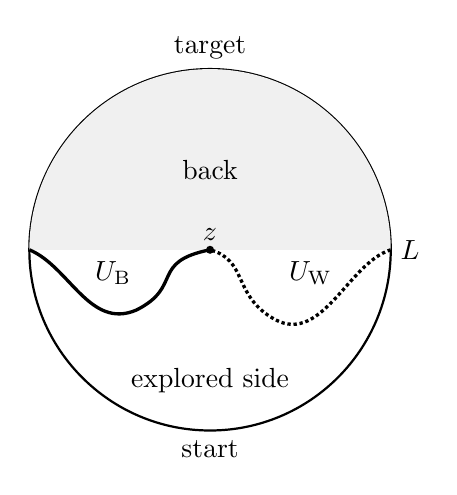
\begin{tikzpicture}[scale=0.85]
  \draw[thick] (0,0) circle (2.7);
  \draw[dashed] (-2.7,0)--(2.7,0);
  \fill[gray!12] (-2.7,0) arc[start angle=180,end angle=0,radius=2.7]
       --cycle;
  \draw[very thick] (-2.7,0) .. controls (-2.1,-.25) and (-1.8,-1.2) ..
       (-1.1,-.9) .. controls (-.4,-.55) and (-.9,-.18) .. (0,0);
  \draw[very thick,densely dotted] (2.7,0) .. controls (2.05,-.2) and
       (1.65,-1.5) .. (.9,-1) .. controls (.35,-.65) and (.55,-.15) .. (0,0);
  \fill (0,0) circle (.06);
  \node[above] at (0,0) {$z$};
  \node at (0,1.2) {back};
  \node at (-1.45,-.35) {$U_{\mathrm B}$};
  \node at (1.5,-.35) {$U_{\mathrm W}$};
  \node[below] at (0,-2.7) {start};
  \node[above] at (0,2.7) {target};
  \node[right] at (2.7,0) {$L$};
  \node at (0,-1.95) {explored side};
\end{tikzpicture}
\caption{The stopped target domain in current disk coordinates,
schematically.  The two side domains $U_{\mathrm B},U_{\mathrm W}$
attach to the back along the open parts of $L$ on either side of the
hit $z$.  Their simple colored boundary arcs may touch in physical
projection; the accesses in the displayed boundary order remain
distinct.  The picture suppresses portions already cut off by the
exploration.}
\label{fig:stopped-domain}
\end{figure}

We now identify the law of these domains.  The argument also applies
when the preceding coordinate map has a nonsimple boundary image,
provided its two banks are separately simple and its closed-disk maps
converge uniformly.  This qualification matters after the first stop.

\begin{lemma}[Cardy determines the stopped kernel]
\label{lem:stopped-kernel}
The joint limiting law of the hit on $L$ and the two side domains of
Lemma~\ref{lem:stopped-domain} is uniquely determined by the scalar
Cardy limits.  For a semicircle cut in coordinates with start $0$ and
target $\infty$, it is the law of chordal $\mathrm{SLE}_6$ stopped
when it first reaches that semicircle.
\end{lemma}

\begin{proof}
First fix a mark in the interior of $L$.  The event of a black
connection from the black bank to the separator between that mark
and the white end forces the hit to the corresponding side of the
mark.  The complementary white connection gives the reverse bound.
This is the elementary Hex separation in the front disk: the two
colored paths along the explored banks terminate at the neighbors
of the first separator vertex about to be queried.  The white
path separates the black bank from separator accesses beyond that
vertex toward the white end, and the black path gives the symmetric
separation.  The comparison is used with a small slack at the
mark, so no identity for the individual terminal triangle is
needed.

These two comparisons are within the scope of the scalar theorem.
Trim each target arc slightly short of its endpoints, and crop a
subdisk connecting it to its mate before extending the targets for
a lower crossing bound.  One target lies on a separately simple
bank and the other lies in the interior separator.  Their cropped
test has Jordan image and stays off the other boundary accesses.
The Jordan sandwich of Lemma~\ref{lem:good-sequences} and
the conformal-coordinate conclusion of Lemma~\ref{lem:chart-cardy}
apply to it.  In particular this is
not an application of Cardy's theorem to an unidentified covering
surface.  As the cropping and the slack decrease, the two bounds
approach the complementary Cardy values.  End stops are negligible:
the endpoint is on an open monochromatic bank away from the
switches, and an approach there carries a free arm of the opposite
color out of its neighborhood.  The limiting hit distribution is
therefore Cardy's hitting distribution and has no atoms.  The same
argument works for piecewise smooth indentations of $L$.

To determine more than the hit marginal, attach finitely many closed
Jordan bumps to disjoint subintervals of $L$ on its front side.
Their sides are simple piecewise smooth curves, and except for their
feet the bumps are interior.  Keep a specified interval of possible
hits disjoint from all feet.  Replace the relevant pieces of $L$
by the bump sides.  The preceding hitting argument determines the
limiting probability of reaching the retained interval on this
indented separator.  On this event the exploration has avoided the
bumps and the retained hit is also its original hit on $L$.

The comparison can be made on the same graph and the same bits.
Approximate the bump sides by simple graph paths in the front disk,
joining the separator in order.  These paths agree with the old
separator away from shrinking neighborhoods of the junctions.
Approach each junction from an interior portion of the bump side
and trim at the original crosscut; the endpoint vertices may vary
inside those shrinking neighborhoods.  There is consequently no
requirement to approximate a prescribed smooth arc through a
prescribed microscopic vertex.  These nested graph separators
really hide the bump interiors from the original start side.
Before querying a vertex on the new separator the exploration
cannot query a hidden part of the old one.  On the unchanged
retained interval the stopping rules agree.

It follows that the indented Cardy value lies between the limiting
probability of strict inclusion of the bumps in the side domains,
with hit in the open retained interval, and the probability of
inclusion in their closures, with hit in the closed interval.
Here \emph{strict inclusion} means inclusion with positive clearance
from the side boundary, allowing the foot to continue through its
open seam.  Conversely strict inclusion and the retained hit force
the indented test to pass, by the domain convergence of
Lemma~\ref{lem:stopped-domain}.  Enlarge the bumps slightly by
regular parallel or polygonal approximations.  Inclusion of an
enlarged closed bump implies strict inclusion of the original;
the Cardy values converge as the enlargement decreases.  Since
hit endpoints have zero mass, these sandwiches determine the
strict inclusion probabilities.  The hit's position relative to
each foot specifies which side domain contains that bump.

These tests determine both open domains, including their joint law.
Indeed a rational ball compactly contained in a side domain can
be joined to its open seam by a polygonal finger of positive width
whose closure stays in that domain.  A countable collection of
rational fingers and balls tests all such inclusions.  Finite
intersections are still bump tests: slightly enlarge overlapping
bumps on the same side, fuse them, fill bounded holes, and fill
pockets against the intervening seam intervals.  Their containing
side domain is Jordan, so these fillings are forced by inclusion.
Under strict inclusion the enlargement can be taken with positive
clearance.  Bumps from opposite sides that intersect are
incompatible; a filling that covers the retained hit likewise
gives an empty event.  Subdivide the retained hit intervals to
distinguish these cases.  Thus the preceding probabilities give a
measure-determining class.  The simple boundaries then recover
the two ordered arcs from their open domains.

Finally compare this characterized law to the classical SLE law in
a round disk.  The Cardy hitting and hull-avoidance characterization
is stated in \cite[Section~5, equations~(8)--(9), and
Lemma~5.1]{cnexploration}.  The single-semicircle hulls have the
side-boundary and first-contact properties just used; these may
also be read from the ordinary triangular-lattice coupling in
\cite[Lemmas~6.3--6.4 and Theorem~5]{cnexploration}.  Here this
last result is used solely to supply properties of the established
$\mathrm{SLE}_6$ law in the standard Jordan setting.  For that
law the indented test is precisely hitting the retained interval
before the bumps, so it has the same Cardy value.  The
measure-determining argument identifies our kernel with that SLE
kernel.
\end{proof}

\subsection{Iteration and recovery of the ordered path}

After a stop, explore in the target face using the boundary colors
already supplied by the same band.  Conditional on all previous
queries, its unknown colors are still independent and fair.  There
is nevertheless a geometric condition to verify before applying
Lemma~\ref{lem:stopped-kernel} again: the two physical banks of the
new domain must remain separately simple.  Uniform convergence of
the maps alone would not imply this.

View all finitely many stopped bands in the initial Jordan disk
coordinates.  They constitute the original exploration continued
in its target face; no additional sites have been queried in advance.
Thus the face-boundary contact rules of
Lemma~\ref{lem:exploration-contacts} still apply.  A bulk self-return
of one colored arc would force six arms, and a self-return at an
original bank is excluded by the corresponding boundary rules.
The remaining possibility involves the terminal point of an arc
at one of the stops.  The hit is in the interior of the preceding
crosscut, and hence strictly inside the preceding physical domain.
Its map is one-to-one in a neighborhood of that point.  The
single-step simplicity conclusion therefore excludes such a return
as well.  At the original target use the fixed-point rule.  This
proves separate bank simplicity at every fixed finite stage; it
does not claim that arbitrary pairs of touching arcs could be glued
to make an admissible domain.

The one-step convergence proved above holds along every
deterministic converging sequence of inputs satisfying these
conditions.  It therefore iterates under bounded integration.
Explicitly, couple the finitely many preceding domains, marks, and
maps to converge almost surely along a subsequence.  Conditional
on these data, the next colors have the product law on the
unqueried sites.  For almost every converging input sequence the
one-step conditional law converges to the stated SLE kernel.
Bounded convergence then gives the next joint law.  Crosscuts may
be chosen measurably, for example by taking the first graph
approximation in a fixed enumeration meeting the prescribed
clearance and order conditions.

In upper half-plane coordinates normalize each new map at infinity
with derivative one, then translate the new start to $0$.  The
domains in these coordinates agree with the half-plane near
infinity throughout a step, so reflection there makes this
normalization continuous.  No boundary derivative in physical
coordinates is used.  For each fixed cut radius $v>0$ and each
fixed number of steps, the sampled target domains and tips
therefore converge to the corresponding samples of chordal
$\mathrm{SLE}_6$, by its domain Markov property.

It remains to show that identifying these samples identifies the
whole curve.  A small capacity increment alone would not suffice:
one must exclude an excursion invisible to the sampled hulls.
We give this last argument explicitly.

\begin{lemma}[No disconnection at a new interior tip]
\label{lem:new-tip-disconnection}
Let a continuous chordal curve in a Jordan disk generate its filled
target hulls.  At a finite time before its first visit to the target,
at which its tip is interior and has
not been visited previously, no point at positive distance from the
trace up to that time and from the initial boundary can become
disconnected from the target for the first time.
\end{lemma}

\begin{proof}
Fix such a point $w$ and time $t$.  Take a small open boundary arc
around the target whose neighborhood is disjoint from the trace up
to time $t$.  Allow connections through that arc to the exterior,
and include the complementary closed boundary arc in the
obstruction.  The obstruction $K_t$ is the image of a continuous
curve obtained by traversing that closed arc and then the
exploration.  Its endpoint, the current tip, is visited only once.
Disconnection of $w$ from the target is now separation of $w$ from
infinity by $K_t$.

We need a small local-connectivity observation with the terminal
point excluded.  For every $\rho>0$ there is $d>0$ such that any
two points of $K_t$ other than its endpoint at distance less than
$d$ can be joined on $K_t$ by a path of diameter less than $\rho$
contained in some strictly earlier obstruction.  Otherwise take
counterexample pairs converging to a common point and their curve
parameters converging to limiting parameters.  If both limiting
parameters are terminal, the short terminal subpath joins the
pair.  If neither is terminal, join each point along its short
parameter subpath to the common limiting value and concatenate;
both subpaths lie strictly before the terminal time.  The mixed
case would give an earlier visit to the endpoint, contrary to the
assumption.  Uniform continuity proves the claimed diameter
bound in each case, a contradiction.

If $K_t$ separates $w$, polygonal closed walks of nonzero winding
number about $w$ can be drawn arbitrarily close to $K_t$.
For example take a fine square grid in general position, form the
union of closed squares meeting $K_t$, and trace the boundary of
the bounded complementary component containing $w$.  Choose the
grid finer than a fixed fraction of $\dist(w,K_t)$.  Subdivide
such a walk, replace its vertices by nearby points of $K_t$ other
than the endpoint, and join consecutive replacement points by
the small paths just constructed.  The resulting closed walk
has the same winding number: each replacement remains in a
small neighborhood avoiding $w$, and can be joined to the
original small segment there.  It consists of finitely many
paths, each lying strictly before time $t$, and is therefore
contained in $K_{t'}$ for some $t'<t$.  Nonzero winding implies
that $K_{t'}$ already separated $w$.  This contradicts first
disconnection at $t$.
\end{proof}

\begin{lemma}[Sampled target domains determine the curve]
\label{lem:no-hidden-excursions}
Every subsequential limit of the exploration in
Proposition~\ref{prop:chordal} has the law of chordal
$\mathrm{SLE}_6$ as an ordered curve.
\end{lemma}

\begin{proof}
Let $\gamma$ be such a limit, in the initial disk coordinates.
For a fixed sampling radius $v$, couple its countably many sampled
domains with an SLE trace $\xi$ having their law; the latter can
be sampled conditionally on the domains.  A diagonal extraction
over finite numbers of steps gives all the samples in their order
on $\gamma$.  At every sample, the path passes through its tip,
the preceding part of $\gamma$ avoids the open target domain,
and the following part lies in its closure.  These are direct
limits of the corresponding band inclusions, using the domain
convergence above.

For fixed $v$, the SLE capacity increments between samples are
independent and identically distributed, strictly positive, and
bounded above by $Cv^2$.  The upper bound is the elementary
half-plane capacity bound for a hull contained in a half-disk of
radius $v$; positivity and independence follow from the
nonconstant chordal SLE trace and its domain Markov property with
the stated normalization.  Their sums therefore diverge almost
surely.  SLE continuity at the start and transience to its target
allow its time interval to be compactified, with the target as
the final point.

Take a sequence $v\downarrow0$.  For each $v$ retain the closed
monotone correspondence between the positions of the samples
on the parameter intervals of $\gamma$ and $\xi$, including
both endpoint pairs.  Take a subsequential Hausdorff limit of
these correspondences, using tight parametrizations of the two
curves.  At the same time retain, at every rational SLE time
$s$, both the compact closure $\overline{D_s}$ of the SLE target
domain and its closed complement.  Encoding both is necessary
to pass the two band inclusions.  The joint law of the SLE curve
with these closed sets is independent of $v$, so every subsequential
limit retains the target domains of its SLE coordinate.  No continuity
of the map from traces to target domains is needed.  The sample capacity gaps are
at most $Cv^2$; hence the limiting correspondence has full
projection on the SLE parameter interval.  Its paired points
coincide in space.  Tail sample pairs accumulate at the target,
so the final endpoint causes no missing projection.

SLE has no constant time interval.  A value of the $\gamma$
parameter cannot therefore be paired with two distinct SLE
times.  Any interval missing from the first projection has its
two endpoints paired with the same SLE time $t$.  If the
correspondence does not already identify the two curves up to
pauses, there is consequently a nonconstant excursion of
$\gamma$ that leaves and returns to $\xi(t)$ inside such a
missing interval.  Every point $w$ on this excursion satisfies
\begin{equation}
\label{eq:hidden-excursion-location}
 w\in\bigcap_{s<t}\overline{D_s},
 \qquad
 w\notin\bigcup_{s>t}D_s.
\end{equation}
It suffices here to use rational $s$.  For the first inclusion,
apply the suffix condition at a sample between $s$ and $t$;
for the second, use the prefix condition at a sample between
$t$ and $s$.  Monotonicity of the target domains and the retained
closed sets pass these conditions to the limit.

If $\xi(t)$ is on the initial boundary, the excursion violates
the absence of a boundary double visit of $\gamma$.  If it is
interior and also visited by SLE at another time, the full
projection of the correspondence supplies a third visit of
$\gamma$ in addition to the two excursion endpoints.  This
violates the absence of interior triple points.  We are left
with a uniquely visited interior tip.

A point satisfying \eqref{eq:hidden-excursion-location} that is
off the SLE trace and off the initial boundary would have
disconnection time exactly $t$.  Indeed it has a neighborhood
free of trace; while a connection to the target exists, a compact
connecting path remains open for a short later time.  The two
inclusions say respectively that disconnection has not happened
earlier and that it has happened immediately afterward.
Lemma~\ref{lem:new-tip-disconnection} excludes this possibility
at a uniquely visited interior tip.  The hidden excursion must
therefore lie entirely on the SLE trace or the initial boundary.

Take a small interior neighborhood of $\xi(t)$.  Every other
point of the hidden excursion there that lies on the SLE trace
has another visit supplied by the correspondence, and is a
double point of $\gamma$.  A nonconstant excursion leaving
$\xi(t)$ must cross one of a fixed countable collection of
line segments forming arbitrarily fine rational grids inside
this neighborhood.  That crossing would be an interior double
point on a fixed segment, excluded by
Lemma~\ref{lem:exploration-contacts}.  Thus the excursion is
constant.  No missing nonconstant interval remains, and the
ordered curve is SLE.
\end{proof}

Lemmas~\ref{lem:exploration-tightness} and~\ref{lem:no-hidden-excursions}
prove Proposition~\ref{prop:chordal}.  Notice that the proof gives
convergence along every deterministic sequence of Jordan graph
domains with ordered boundary convergence, which is the form needed
to explore the random faces below.

\subsection{Restoring a virtual bank and exploring loops}

We now work in a large Jordan disk, with all eventual crossing tests a
positive distance from its boundary.  Initially give its boundary a
single color.  The disk may be approximated by internally chord-free
site cycles.  Changing boundary colors on that cycle does not change
the original fair colors of sites in the region of the tests.

The continuum object used here is the oriented percolation-loop
construction of Camia and Newman \cite{cnloops}: successive chordal
$\mathrm{SLE}_6$ explorations in Jordan domains, with the two sides of
each interface assigned their colors.  We recall the discrete
construction sufficiently precisely to verify that it has this limit.

With actual two-switch boundary conditions, explore and retain the
monochromatic unknown faces of Lemma~\ref{lem:revealed-faces}.
Inside a face with constant boundary color, temporarily change one
boundary bank to the opposite color and make a chordal exploration.
We call that changed bank \emph{virtual}, because its original color
is restored afterward.  For definiteness suppose its virtual color
is black and its actual color white.  Excursions away from the virtual
bank supply pieces of actual interfaces; further explorations in
the faces incident with that bank complete those pieces to loops.
The following incidence description specifies the completion, including
faces attached at only one site.

\begin{lemma}[Restoration and ordered excursions]
\label{lem:virtual-restoration}
Restoring a virtual boundary bank pairs its excursions with
explorations of the incident unknown faces according to their order
along the bank.  For every fixed positive diameter cutoff, the
excursions, the incident faces used to complete them, and their
completed oriented loops converge jointly.  No macroscopic loop
is produced in the limit solely by excursions or incident faces of
vanishing size at this step.  Conditional on the exposed boundaries,
all still unknown interior colors remain independent and fair.
\end{lemma}

\begin{proof}
First work at a fixed mesh, with a virtual black bank whose
actual color is white.  List the edges from that bank to revealed
vertices off the bank, including the switch edges.  Order them
along the bank and then within successive interior vertex stars.
Thus several entries may use one bank vertex.  Label each entry
by the color of its \emph{off-bank endpoint}.  The white entries
are exactly the places where the virtual wall crosses a
bank-incident edge.  Their order along the wall is the bank/star
order: the short spokes joining them to the bank lie on one side
of the simple wall and cannot cross.

Between two consecutive white entries the list has the form
\[
             W_i,B_1,\ldots,B_k,W_{i+1}.
\]
Write $E_i$ for the virtual excursion between those white entries
and $I_i$ for the intervening bank interval, retaining the star
order if the interval is a single vertex.  Apart from its end
triangles, $E_i$ is an actual interface after restoration.
We describe the returning chain that completes it.

Consecutive entries bound a common face, possibly a triangle,
because there are no rim chords and every incident face has a
single bank interval or vertex by Lemma~\ref{lem:revealed-faces}.
For $k>0$, each middle wedge $B_j,B_{j+1}$ is a triangle or an
unknown face whose boundary is black before restoration.
Restoring the bank to white creates exactly two switches there.
Join them directly through the triangle, or by exploring that
unknown face with its actual two-switch boundary conditions.
The end wedges $W_i,B_1$ and $B_k,W_{i+1}$ have mixed colors
before restoration, so they cannot be unknown monochromatic
faces; they are band triangles.  After restoration they join
the returning chain to the surviving ends of $E_i$.  Consequently
a nonempty run completes that same excursion to one real loop.
An empty run through only bank triangles has no macroscopic
contribution.  White entries separate different runs, so this
operation cannot concatenate distinct excursions.  Unused interfaces lie in the other unknown
faces, including residual faces of these closing explorations.
This is a finite incidence identity; it asserts no independence
of the virtual excursions.

We next show that the identity passes to the limit.  Work in
the initial disk coordinates of this step.  A sequence of
excursions of diameter bounded below has, by curve tightness,
a limiting pair of endpoints and an ordered limiting arc.
Its interior cannot acquire a contact with the virtual bank:
during the discrete excursion neither bank shadow uses that
bank, so such a contact between positive excursions gives
three free half-plane arms as in
Lemma~\ref{lem:exploration-contacts}.  Conversely a compact
subarc that avoids the bank in the limit eventually avoids it
discretely.  There is no boundary interval of the limiting wall,
no boundary double visit, and no return at a switch.  Hence
positive-size excursions have distinct endpoints and match in
their order; no positive excursion can collapse to a spike
at one boundary point.

Every limiting contact with the open bank is approximated by
an actual recorded occurrence, not just the contacts selected
by a diameter cutoff.  Otherwise the approaching and departing
wall segments in an occurrence-free neighborhood would give
the same three-arm event.  Together with the initial and final
bank points, this recovers the full order of the contacts.

For a matched excursion, the intervening bank interval is
incident with one limiting face of positive size.  Every
compact subinterval of that interval has an adjacent strip
avoiding the band; its limiting face has a Jordan boundary by
Lemma~\ref{lem:face-convergence}.  Its two attachments converge
to the excursion endpoints, so its actual two-switch marks
also converge.  Proposition~\ref{prop:chordal} supplies the
closing exploration.  Any other incident faces involved in
that run have attachments collapsing to the endpoint
neighborhoods.  Their diameters tend to zero: a positive
diameter face of the virtual bank's color with a collapsing
attachment interval, including a singleton, is excluded by
Lemma~\ref{lem:exploration-contacts}.  Thus their pieces cause
no error in the curve metric when the loop is pasted.

The same argument rules out a surplus macroscopic loop
completed from vanishing excursions at this step.  If $E_i$
shrinks, its endpoints coalesce, and continuity of the inverse
Jordan-bank parametrization makes $I_i$ shrink as well.  Every
completion face for this run is attached to $I_i$; all its band
triangles are within a vanishing mesh distance of that interval.
The diameter of the completed loop is therefore bounded by the
diameter of $E_i$, the diameter of $I_i$, twice the largest
completion-face diameter, and a vanishing mesh error.  The
collapsing-attachment exclusion makes that largest diameter tend
to zero.  This also excludes an accumulation of many small
completion pieces into a macroscopic loop.
An other-colored face whose boundary merely
touches the bank in the limit, without genuine cycle edges
on it, receives no new switch assignment.  True intervals of
attachment have been distinguished by
Lemma~\ref{lem:face-convergence}.  This distinction prevents
an incorrect extra reconnection at a limiting contact.

Actual two-switch explorations leave monochromatic faces
again.  Their unknown sites are fresh conditional on all
queried colors by the product-law argument preceding
Lemma~\ref{lem:revealed-faces}.  Select and match faces, for
example, using interior points from a fixed dense countable
set that avoid the traces.  Along every deterministic
converging sequence of selected Jordan faces,
Proposition~\ref{prop:chordal} applies.  The bounded-integration
argument used for stopped kernels therefore gives joint
convergence of each finite set of operations.  Uniform
continuity of the Jordan coordinate maps transfers all these
statements back to physical coordinates.
\end{proof}

\begin{proposition}[Oriented loop convergence]
\label{prop:loops}
In a Jordan disk with monochromatic boundary, along every
deterministic sequence of tilings under consideration, the
critical interface loops converge to the Camia--Newman
$\mathrm{SLE}_6$ loop construction.  For each positive cutoff
chosen outside the atoms of limiting loop diameters, the loops
above that cutoff can be matched in the curve metric, including
their orientation, multiplicity, and order of excursions.
There are no surplus macroscopic loops.  The convergence holds
jointly for any finite number of independent color replicas
on the same fixed geometry.
\end{proposition}

\begin{proof}
Lemma~\ref{lem:virtual-restoration}, iterated, proves convergence
of every fixed finite number of recursive operations.  It
remains to justify that finitely many operations discover all
loops above a fixed scale with arbitrarily high probability.
We use a property of the already identified continuum SLE
construction, checking its precise scope.

Fix a conformal map from the unit disk onto the initial Jordan
domain, extended as a homeomorphism of closures.  In these
initial disk coordinates choose the exploration order and
boundary endpoints as in \cite[Section~3.2]{cnloops}: priority
is by maximal coordinate span, with its specified dense-point
tie breaking; monochromatic domains use the maximal-span
endpoint rule, and two-color excursion domains use their two
prescribed switches.  Start with that construction's
monochromatic disk and virtual first exploration and transport
the recursion by the fixed map.  For this continuum recursion
the number of steps until every remaining domain has
coordinate diameter below a fixed $r>0$ is almost surely
finite.  Here is the exact consequence of \cite{cnloops}
that proves this assertion.  Theorem~5 there gives finite-step
coupling with the reorganized triangular construction, and
its proof, equation~(20), proves tightness of the stronger
triangular stopping count until all remaining domains have
coordinate span below a prescribed cutoff.  The final part
of that proof transfers this estimate from the original
construction to the reorganized one by its maximal-span
comparison.

To pass that statement to the continuum, suppose that after
$n$ steps a continuum remaining domain has diameter greater
than $r$.  Choose a compact connected subset of its interior
with diameter greater than $r-z$, by joining two interior
points with a compact path.  This subset has positive distance
from the finitely many explored boundaries.  Under the
finite-step coupling it stays in a corresponding triangular
remaining domain for all sufficiently small lattice meshes.
Hence that triangular domain has diameter greater than
$r-z$, and its coordinate span exceeds
$(r-z)/\sqrt{2}$.  Taking the mesh limit in the tight
stopping-count estimate, and then $n\to\infty$, proves the
continuum assertion, using a smaller cutoff to obtain the
strict diameter inequality.  This use of the triangular theorem
establishes a fact about the known continuum SLE recursion;
it supplies no convergence assertion for the present
tessellations.

Uniform continuity of the fixed initial conformal map converts
this coordinate exhaustion into exhaustion at every positive
physical diameter.  We may now couple finitely many steps of our construction
to those continuum choices.  On each matched boundary choose
the nearest ordered discrete endpoints.  The choice depends
only on the coupled past, so it leaves the unknown discrete
colors with their correct conditional product law.  This
avoids imposing an unwarranted continuity assumption on a
maximizing endpoint rule.  At each step
Lemma~\ref{lem:face-convergence} matches the remaining
macroscopic faces with no surplus.  Induction gives that
property after every fixed finite number of operations.

Fix an error probability and first choose, using continuum
exhaustion, a deterministic number of operations after which
all continuum remaining faces are smaller than the desired
cutoff with the stated high probability.  If an excursion
already drawn still needs its matching face exploration to
complete a macroscopic loop, perform those additional
operations as well.  For each positive excursion cutoff
there are only finitely many such mates; include all of
them and then decrease this auxiliary cutoff.  The
no-surplus assertion of Lemma~\ref{lem:virtual-restoration}
ensures that vanishing excursions at any of these finitely
many steps cannot produce a missing macroscopic loop.
All other loops lie within the remaining small faces.
Finite-step convergence now gives the required loop matching,
and then the error probability and auxiliary cutoffs may
decrease.  The incidence rule retains orientation and
multiplicity throughout.  Finally, on deterministic geometry
different replicas have independent colors, so their finite
recursive laws are independent products; the same limiting
and cutoff arguments give their joint convergence.
\end{proof}

We have obtained a common critical loop law from the scalar
crossing limit, with the fixed geometry retained throughout
each exploration.  To use it in the near-critical expansion,
we next read the prescribed polygon crossings from these
loops and allow finitely many fixed squares to be forced to
specified colors.

\section{Joint crossings and prescribed regions}
\label{sec:critical-tests}

Section~\ref{sec:critical} identifies the oriented critical loops along
each deterministic good sequence.  We now prove convergence of the
observables needed for the near-critical argument: finite collections
of polygon crossings after several separated squares have been forced
black or white.  First we recover the literal crossings confined to
each polygon from the oriented loops.  We then combine continuity under
small motions of the prescribed regions with finite witnesses made of
ordinary polygon crossings.  Proposition~\ref{prop:critical-tests}
collects the resulting common joint law, including its conditional
version for Poisson geometry.

\subsection{Reading joint crossing tests from the loops}
\label{subsec:critical-readout}

An interface may enter and leave a quad repeatedly.  We therefore
determine the quad crossing from the boundary pairing of interface
portions inside it.

Write the sides of a quad in boundary order as $S_1,S_2,S_3,S_4$, with
$S_1,S_3$ the black target sides. At a finite mesh, draw the interfaces along
cell edges, retaining their orientations and hence the color on each bank.
In general position with respect to a polygon, their portions in its interior
are disjoint crosscuts and closed curves. The following elementary rule reads
the crossing from these portions.

\begin{lemma}[Boundary-pairing rule]\label{lem:boundary-pairing}
Suppose finitely many disjoint interfaces, with their two bank colors, cut a
Jordan quad, avoid its marks, and cross its boundary whenever they meet it.
If an interface crosscut joins $S_1$ to $S_3$, the black bank supplies a black
crossing. If one joins $S_2$ to $S_4$, the white bank supplies a complementary
white crossing. If neither type occurs, there is a complementary region
incident to all four sides; its color determines the crossing. Whenever a
crosscut joins the two sides incident to a mark, the orientation of the
outermost such corner cut determines this central color.
\end{lemma}

\begin{proof}
A crosscut between opposite sides separates the other pair. Paths running
arbitrarily close to its banks give the asserted color connections; they can
be taken with clearance on their respective sides. The two types of opposite
crosscut cannot coexist, because they would intersect.

In their absence every crosscut has both ends on one side or on consecutive
sides. On the boundary circle the endpoint pairing is noncrossing. A same-side
pair cuts off a pocket containing no mark. A pair on consecutive sides cuts
off the corresponding corner. Remove the pockets and, for each corner that
is cut off, its outermost corner pocket. The remaining region is connected
and incident to each of the four side intervals between the removed pockets.
This can also be proved by induction: remove an innermost paired interval
first, then restore it as a pocket along one boundary interval of the remaining
region. Interior closed curves only remove interior pockets. Consequently the
region left between the corner pockets meets all four sides. A path through
it joins either pair of sides, and its color decides which crossing occurs.
The bank of an outermost corner cut facing this region has that color.
All paths used here lie in the quad; no identification of different boundary
points or external connection is made.
\end{proof}

We explain why this finite rule is stable for the limiting loops. First put
the polygon in general position by a translation chosen from an arbitrarily
small open disk. For almost every such translation, almost surely the limit
loops avoid the vertices and marks, have no double point or mutual contact on
a side, and have no tangency there that is a local extremum of the coordinate
normal to the side. Here are the estimates and deterministic facts behind
these assertions. A prescribed point is avoided by the one-arm estimate.
A double visit or a contact of two loops on a line segment produces four
traversals in a ball centered on that segment. Covering the segment by
$O(r^{-1})$ balls and using Lemma~\ref{lem:color-arms} gives an upper bound
$O(r^{c})$, for some $c>0$, when the traversals continue to a fixed positive
distance. Let that distance run through a countable sequence and then let
$r\downarrow0$. Finally, for any continuous real function, the set of its
local-maximum and local-minimum values is countable: each such value is the
maximum or minimum on some interval with rational endpoints. Apply this to
the normal coordinate along each of the countably many loops. Almost every
translation avoids all those levels. These facts hold simultaneously for a
finite collection of polygons. General position at finite meshes is obtained
by excluding a further null set of translations; at a Voronoi vertex the
incident cells are pairwise side-adjacent, so this exclusion introduces no
new connectivity convention.

There are also corner cuts at positive, possibly random, distances from each
mark. To see this, choose many disjoint buffered annuli around the mark, all
small enough that the two incident polygon sides are the only boundary pieces
present. In each annulus, fixed crossing chains give a black circuit and a
white circuit in separated subannuli with a probability bounded below.
The colors in these buffered regions are independent on a deterministic
mesh, once the mesh is sufficiently small. Thus the probability that none
of $k$ annuli supplies the circuits is at most $(1-c)^k$. The two circuits
force an intervening closed wall enclosing the mark. Following this wall
through the polygonal sector gives a cut between the incident sides.
Take the mesh limit first and then $k\to\infty$. This proves the claim also
when the mark lies in the interior of a straight side.

Fix one such cut at each mark, and trim its two reaches on the incident sides
a positive distance away from that mark. Any outermost corner cut beyond
these reaches has positive diameter: the two compact side portions in
question are disjoint. Opposite-side excursions also have positive diameter
after the mark neighborhoods have been removed. At any fixed positive reach
there are only finitely many relevant excursions, by curve continuity and
the finite macroscopic matching in Proposition~\ref{prop:loops}. Their orders
and bank colors persist under convergence. Indeed their compact interior
portions stay in the open quad. At an endpoint on a side, the loop must
approach the line from both sides in every sufficiently small parameter
neighborhood, unless that line is a local-extremum level. Therefore nearby
curves recover the endpoint crossing. Conversely, a sequence of excursions
of positive reach has a limiting excursion: it cannot collapse at a mark,
and it cannot acquire an intermediate boundary contact without either a
double contact on the side or a forbidden one-sided tangency. Reach cutoffs
can be chosen to avoid equality. The boundary-pairing rule now gives the same
crossing decision on matched configurations. Unmatched loops of vanishing
diameter cannot change it, because the positive corner reaches have already
fixed the central color in the case with no opposite-side excursion.

For a specified, unperturbed polygon use the inner and outer Jordan sandwich
tests from Lemma~\ref{lem:good-sequences}. They are chosen so that, on the same
colors, the lower crossing implies the specified crossing, which implies
the upper crossing. The tests may be put in the preceding general position.
The difference between their limiting probabilities tends to zero with the
sandwich width, by continuity of Cardy's formula under convergence of the
marked Jordan boundaries. A union bound applies to any finite family. We
have therefore proved joint convergence of the exact closed-cell crossing
indicators, along every deterministic good sequence, to a common critical
law. This argument also proves convergence for polygonal site-path tests
with the terminal conventions of Section~\ref{sec:critical}: the positive
sandwich margins absorb the conversion between site paths and cell paths.

\subsection{Continuity under changes of prescribed regions}
\label{subsec:forced-continuity}

Fix a finite family of closed squares
\[
 H_j=\{x\in\RR^2:\|x-z_j\|_\infty\le h_j\},\qquad h_j>0,
 \quad 1\le j\le J.
\]
Assume that the squares are mutually disjoint at positive distance and that
each is at positive distance from every polygon boundary under consideration.
For each crossing test choose, separately, whether to force all cells meeting
$H_j$ black, to force them white, or to leave them unchanged. A square outside
a particular quad is irrelevant once the mesh is small. Different tests may
make different choices while using the same original fair colors. If a cell meets two differently prescribed squares, assign it the color of
the square with smaller index; this convention is eventually irrelevant on
a good sequence, since the squares have positive separation. Throughout
this subsection the number of squares, their positive radii, and their
separations are fixed before the mesh tends to zero.

Call an arm \emph{free} when it uses only sites whose original fair colors
have not been prescribed in the test. We will use the mesh-first bounds
\begin{equation}\label{eq:forced-arm-bounds}
\begin{aligned}
 \limsup_{e\to0}\PP(\hbox{one free arm from }r\hbox{ to }R)
       &\le C(r/R)^\gamma,\\
 \limsup_{e\to0}\PP(\hbox{three free half-plane arms})
       &\le C(r/R)^\beta,
\end{aligned}
\end{equation}
where $\gamma>0$ and $\beta>1$; the second bound allows any color order and
any fixed side direction. These are consequences of
Lemmas~\ref{lem:arm-inputs} and~\ref{lem:boundary-arms}. Shifts of the bounding
line and constant factors in the radii are allowed. All probabilities in the
next two lemmas are color probabilities on a deterministic good sequence.

\begin{lemma}[Continuity of prescribed-region tests]
\label{lem:forced-continuity}
For any fixed finite family of polygon crossing tests with the square
prescriptions above, the probability that a test changes under a sufficiently
small polygonal displacement of its sides, marks, or prescribed squares tends
to zero, uniformly in the mesh-first limit. The displacements may change the
centers and positive side lengths of the squares, provided the stated
separations persist. The same conclusion holds simultaneously for any fixed
finite collection of prescription choices on the same colors.
\end{lemma}

\begin{proof}
We give both the geometric interpolation and the arm test for a single local
change. Choose $u>0$ smaller than the separations of all unrelated sides and
squares, and put balls of radius $Cu$ around the polygon vertices, marks,
and square corners. Outside these balls divide each straight edge into
$O(s^{-1})$ intervals of length comparable to $s$, where $s\ll u$. For a
displacement much smaller than $s$, perform the motion one interval at a time,
using a piecewise linear cutoff supported on a slightly longer interval.
Leave the portions within distance $2u$ of the vertices for the corner
moves, and taper the edge moves between distances $2u$ and $3u$; motions in
balls of radius $4u$ then complete the interpolation. There are boundedly
many corner moves and $O(s^{-1})$ edge moves. A polygonal collar identifies
the vicinity of each edge with a straight strip. Interpolating its sufficiently
small piecewise linear ambient displacements preserves the Jordan property;
it also gives the familiar quad sandwiches by shifting target and non-target
sides in their respective directions. Squares are treated by the same
construction. Each intermediate prescribed region remains a connected disk,
and the part common to the two regions in a local comparison is connected.
This last property can be ensured by taking the motions to be graphs in their
collars and retaining the unchanged inner square. All constructions are
fixed before $e\to0$.

Consider an edge move supported in a ball of radius $Cs$. If it changes a
crossing, take a black crossing from the configuration where the crossing
occurs and an open white complementary crossing from the other configuration.
Outside the changed neighborhood their paths run in the common tiling and
coloring. For a quad-side move, their portions going to the other three sides
give three disjoint free arms from scale $Cs$ to scale $cu$. They lie in a
half-plane translated by $O(s)$ from the original supporting line. Trimming
at first and last hits of auxiliary curves preserves the order of the arms.
The paths stay in the common region of the two domains; using the enlarged
half-plane therefore does not require the intermediate boundary itself to
be straight.

At an edge of a black prescribed square, the two arms of the white
complementary path are free. At least one of the two black branches towards
the target sides is also free until scale $cu$. Otherwise both target sides
would connect, before entering the changed neighborhood, to the common
black prescribed region. That region is connected also in the comparison
without a crossing, so it would already join the target sides there, a
contradiction. The white branches cannot connect to one another in the common
part so as to avoid the changed region, since they would then block the black
crossing in the other comparison. After proper trimming we thus have three
disjoint free arms in the exterior half-plane of the square edge. A white
prescribed square is handled with the colors interchanged. The open white
connections through a white prescribed region exist with clearance, because
its forced cells form a connected union by side adjacency.

Here and below the ``cells meeting'' convention is compatible with that
connectivity. Follow a path inside the connected prescribed region through
the cells it meets. Consecutive cells share a side, or meet at a tiling vertex
where the three cells are pairwise side-adjacent. The resulting side-adjacency
chain connects all cells meeting the region. A path in those cells can be
moved into cell interiors and relative interiors of shared sides. On an
unchanged straight boundary piece, convexity of each cell and the shortcut
argument for crossing and complementary crossing remove possible reuse of a
cell by two candidate arms. The finitely many bends introduced by a fixed
interpolation require one further observation. A shared cell there, despite
the arms continuing to a fixed outer scale, would give a free arm from a
vanishing neighborhood of that bend to that scale. Its probability tends to
zero by the one-arm bound. Thus the graph-arm extraction is valid with
vanishing error, including for the exact closed-cell crossing convention.

At a corner move, a changed crossing requires at least one free arm from
scale $Cu$ to a fixed positive scale. At a quad vertex or mark this is a
branch of the crossing towards a target arc away from that vertex. At a
prescribed square it is a branch of the color opposite to that square;
this branch cannot use the prescribed region. Since all other prescribed
regions and unrelated boundary pieces are at fixed positive distances,
the arm is free throughout the annulus used for this estimate.

A union bound and \eqref{eq:forced-arm-bounds} give, for displacement small
enough in terms of $u,s$,
\begin{equation}\label{eq:forced-continuity-error}
 \limsup_{e\to0}\PP(\hbox{some compared indicator differs})
 \le C u^\gamma+C s^{-1}(s/u)^\beta.
\end{equation}
Constants may depend on the fixed tests and their separations. The vanishing
errors at the finitely many interpolation vertices have already disappeared
in the mesh limit. Given an error tolerance, first choose $u$ so that the
corner term is small, then choose $s$ so that the edge term is small, and
finally restrict the displacement. Equivalently, in the displayed bound the
limits are taken as $e\to0$, then $s\downarrow0$ at fixed $u$, and then
$u\downarrow0$. This proves the lemma.
\end{proof}

\subsection{Finite witnesses after prescribing square colors}
\label{subsec:forced-witnesses}

Continuity alone does not identify the law of the modified crossings: prescribing
a square does not make its neighboring crossings independent. We instead
show that a positive crossing, after a small favorable perturbation, has a
witness consisting of finitely many ordinary critical polygon crossings.
Those were identified in Subsection~\ref{subsec:critical-readout}.

For a black crossing, a \emph{favorable perturbation} enlarges every black
prescribed square, shrinks every white prescribed square, and makes a quad
sandwich favorable to black. The latter moves its target caps slightly towards
each other and its non-target sides outwards in polygonal collar coordinates.
A path crossing the original quad then crosses the perturbed quad after it
is clipped at the new caps. We use two nested perturbations, called the
middle and final perturbations, with positive slack between each pair.
All prescribed squares remain separated and off the quad boundary.

\begin{lemma}[Free segments of a terminal path]
\label{lem:free-segments}
Discard squares left unchanged in the test and squares outside its quad.
Construct a graph approximation to the middle quad with the remaining
middle squares removed. Give its vertices the original fair colors. Fill each square hole
by a fan from one new vertex having that square's prescribed color, and
attach uncolored terminals to the two target arcs. On the event that the
original modified configuration crosses, this graph has a black terminal
path for all sufficiently small meshes. It has such a path whose portions
between consecutive terminals or fan vertices form at most $J+1$ free paths.
Their joint laws, restricted to the crossing event, are tight in the curve
metric. Every subsequential limiting free path is simple after constant
parameter intervals are removed.
\end{lemma}

\begin{proof}
Approximate the outer boundary and hole boundaries in disjoint thin strips
by simple site cycles, in boundary order, using the graph approximation
construction of Section~\ref{sec:inputs}. Hole rims are free vertices.
The graph outside these cycles, with each hole triangulated by its fan,
is a finite planar triangulation. The terminal neighbors are exactly the
sites on the corresponding target arc; the terminals create no connection
between other boundary vertices.

Shadow an original closed-cell crossing by a site path with vanishing error.
Before it enters a black forced square, it crosses the rim of the enlarged
middle square through free black sites; crop there and replace its subsequent
passage through that square by the black fan. An original black path stays
away from every shrunken white hole. The quad collar slack allows the shadow
to be clipped at the middle target arcs and keeps it clear of the middle
non-target sides. This produces the claimed terminal path. These statements
only use the small mesh of cells on the fixed compact region and the strictly
positive slack, so hold for all sufficiently fine configurations on the
given crossing event.

Choose an outermost black terminal path on one side. More precisely, add an
external edge joining the terminals, take the union of all simple black
terminal paths together with that edge, and take the appropriate exterior
boundary cycle of this union. Each constituent path with the external edge
is a cycle, and these cycles share that edge; their union is two-connected.
Its exterior boundary therefore supplies a simple terminal path $P$.
No black path can leave $P$ into the exterior side and return to a distinct
vertex of $P$: taking its first departure and first return would produce a
terminal path farther on that side, contrary to the boundary construction.
We call this the no-bypass property. It is the same elementary outermost-path
construction used in Lemma~\ref{lem:rectangle-colors}.

A simple $P$ visits each fan vertex at most once and never visits a white
fan vertex. Remove the fan edges and terminal edges. The remaining segments
join distinct rim or terminal sets and consist entirely of free black sites.
There are at most $J+1$ of them. Many traversals of a fixed annulus by one
segment yield equally many disjoint free black arms, after proper trimming.
The one-color disjoint-occurrence bound and the one-arm bound control these
numbers. The successive-excursion compactness argument in
Lemma~\ref{lem:exploration-tightness} consequently applies to these segments,
also at their endpoints. Notice that the segments may be selected using all
the colors; the bound is on the existence of the disjoint arms and does not
assume freshness conditional on the selected path.

We give the additional argument that rules out a self-touch in a limit.
Suppose first that the contact lies in the bulk, at positive distance from
all rims. Two visits with a nonconstant intervening excursion produce four
proper traversals of a sufficiently small annulus, with a fixed positive
outer radius. Between the traversals, on the side forbidden by the
no-bypass property, there are at least two disjoint radial gaps. Indeed, in cyclic order the
four directed traversals have distinct sectors on their forbidden sides;
at most two traversals can border the same such sector. Each selected
gap contains a white arm. To justify the last assertion without assuming
smooth graph cuts, choose two intermediate graph cycles, with wide radial
margins. Within the gap each cycle has a transverse vertex path between its
two path banks. One way to see this is to label just the vertices of that
cycle black and apply Hex in the gap: an avoiding radial white path would
cross the separating cycle, which is impossible. Use an innermost such cut
at the inner cycle, and then one at the outer cycle. They enclose a
quadrilateral whose side banks are portions of $P$. A black crossing between
these banks would leave into the forbidden side and return to $P$; trim at
its first return to obtain a bypass. Hex therefore gives a white crossing
between the transverse cuts. With the cuts chosen away from the trimmed
ends, the departure points on $P$ are internal and both adjacent path edges
are still present, as required for the no-bypass argument. Trim the white
crossing to the smaller annulus. Doing this in the two disjoint gaps yields
four black and two white site-disjoint arms. All vertices involved are free;
no fan edge or rim has entered this annulus.

By Lemma~\ref{lem:color-arms}, the probability of such a six-arm event in any
of $O(r^{-2})$ balls of radius $r$ is $O(r^{c})$, when its outer radius is
fixed. It tends to zero. At a point of a straight rim or outer boundary,
a self-touch gives at least three free traversals in the corresponding
half-plane. There are three even if one of the two visits is an endpoint
of the segment. Covering that side by $O(r^{-1})$ balls and applying
Lemma~\ref{lem:boundary-arms} again gives a vanishing bound. At the finitely
many polygon corners, a single free arm reaching from vanishing scale to a
fixed scale already has probability tending to zero. The endpoints of a
segment lie in distinct, positively separated rim or terminal sets, so they
cannot coincide with each other. These exclusions at countably many outer
scales rule out every nontrivial repeated point of a limiting segment.
\end{proof}

The need for a middle perturbation is now visible; see
Figure~\ref{fig:forced-tube}. A free segment can touch a
middle rim or boundary. The final perturbation puts its black attachment
points inside an open black square and separates it from every final white
square. Thus the segment can be surrounded by a genuine open tube without
having to reconstruct any limiting connectivity at a contact point.

\begin{figure}[t]
\centering
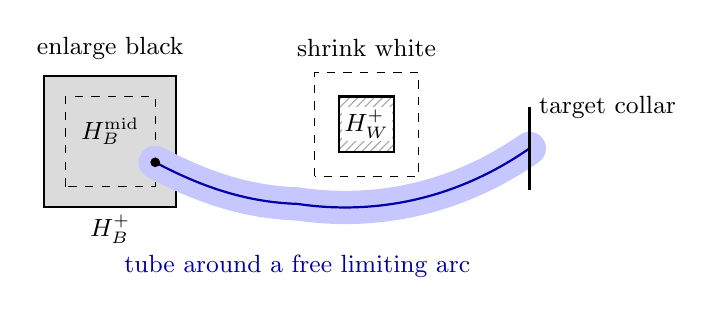
\begin{tikzpicture}[scale=.88,every node/.style={font=\small}]
 \fill[black!14] (.35,.35) rectangle (2.25,2.25);
 \draw[thick] (.35,.35) rectangle (2.25,2.25);
 \draw[dashed] (.65,.65) rectangle (1.95,1.95);
 \node at (1.3,2.65) {enlarge black};
 \node at (1.3,1.45) {$H_B^{\rm mid}$};
 \draw[dashed] (4.25,.8) rectangle (5.75,2.3);
 \fill[pattern=north east lines,pattern color=black!35]
       (4.6,1.15) rectangle (5.4,1.95);
 \draw[thick] (4.6,1.15) rectangle (5.4,1.95);
 \node at (5,2.65) {shrink white};
 \node[fill=white,inner sep=1pt] at (5,1.55) {$H_W^{+}$};
 \draw[blue!22,line width=12pt,line cap=round]
       (1.95,1) .. controls (2.7,.6) and (3.35,.42) .. (4,.4)
       .. controls (5,.25) and (6.2,.4) .. (7.35,1.2);
 \draw[blue!65!black,thick]
       (1.95,1) .. controls (2.7,.6) and (3.35,.42) .. (4,.4)
       .. controls (5,.25) and (6.2,.4) .. (7.35,1.2);
 \fill (1.95,1) circle (2pt);
 \draw[thick] (7.35,.6)--(7.35,1.8);
 \node[right] at (7.35,1.8) {target collar};
 \node[blue!65!black] at (4,-.5) {tube around a free limiting arc};
 \node at (1.3,.04) {$H_B^{+}$};
\end{tikzpicture}
\caption{The middle rims are dashed and the final prescribed squares have
solid boundaries. A limiting free segment starts on the middle black rim,
strictly inside the final black square. Its tube stays clear of the final
white square. Its other endpoint is shown in a target collar. Thus an
ordinary crossing of a polygon quad in the tube can be joined through the
final black region and clipped at the target cap. The figure is schematic;
no regularity of the limiting arc beyond simplicity is used.}
\label{fig:forced-tube}
\end{figure}

\begin{lemma}[Transfer by polygon witnesses]\label{lem:forced-transfer}
Let two deterministic good sequences be coupled so that their ordinary
critical polygon crossing indicators converge jointly to the same indicators
for a countable family containing the rational polygons. For any fixed
prescribed-square test, the probability of a crossing in the first sequence
and no crossing in the final favorable perturbation of the second tends to
zero. The conclusion holds for finitely many tests and for independent
color replicas.
\end{lemma}

\begin{proof}
It suffices to consider a subsequence on which the asserted mismatch has
positive limiting probability. Include its indicator, the crossing vectors,
and the at most $J+1$ segments of Lemma~\ref{lem:free-segments} in a joint
subsequential representation. Pad the segment list when necessary and
include its finite combinatorial itinerary through the hubs as a coordinate
in a finite discrete space. In the representation this itinerary stabilizes
almost surely, though its limit may be random. Tightness gives convergence
of the segment curves;
Lemma~\ref{lem:free-segments} makes each nonempty limit a simple arc.
On the represented mismatch event their ordinary critical crossing vectors
agree in the limit, coordinate by coordinate.

For each limiting segment, choose its two end neighborhoods as follows.
An end at a black hub lies strictly inside the final enlarged black square;
an end at an outer terminal lies in the collar on the appropriate side of
the final target cap. The segment stays a positive distance from the final
white squares, because these are strictly smaller than the middle white
holes. Its non-target boundary approaches have room inside the final
non-target collar. Near the two ends, cut the simple arc at points still
within the prescribed end neighborhoods. The planar Schoenflies theorem gives a rectangular neighborhood of the
intervening simple arc, which can be chosen as a thin tube around it. Choose a polygon quad in this
tube whose target end cuts are inside those neighborhoods and whose lateral
sides leave room around the arc. A sufficiently close rational polygon
approximation preserves these properties. Uniform convergence in curve
order implies that the corresponding free segment in the first model
crosses this fixed quad for all sufficiently large indices.

The witnesses can depend on the limiting configuration, but are selected
from a countable list. On the representation, convergence of a Boolean
coordinate means eventual equality of that coordinate. Thus, simultaneously
for every member of the list, a witnessed black crossing in the first
sequence is also present in the second for all sufficiently large indices.
There are only finitely many witnesses on the event under consideration.
Their crossings in the second sequence avoid its final white squares: the
tube clearance eventually exceeds every cell diameter in the fixed region,
so none of the cells in a tube can be recolored white by a distant square. If
a crossing enters an enlarged black square, that only helps it. At a hub,
the two adjoining witnesses have endpoints in the open square, so the forced
black cells connect them there with clearance. At the outer ends, join in
their prescribed order and clip the resulting path at the final target caps.
This yields a black crossing of the final test, contradicting the represented
mismatch. The tubes need not be disjoint: their only required joins occur
inside their specified black squares, and any additional intersection of
black witnesses is harmless.

For several tests apply this argument to each positive indicator; for an
indicator equal to zero use the same implication in the reverse coupling
when deriving equality of laws. For replicas keep a separate segment list
and crossing vector in each replica. The arm bounds apply separately, and
a finite union bound proves the assertion without any assumption that
the replicas have independent geometries.
\end{proof}

\subsection{The resulting critical comparison}
\label{subsec:critical-comparison}

We collect the precise conclusion needed below. A test specification consists
of a polygon quad, a replica label, and a choice in $\{*,B,W\}$ for each of a
finite family of squares; $*$ means that the original fair colors are left
unchanged. A finite collection of specifications may repeat the same quad
with different prescriptions. Within a replica all tests use the same fair
color configuration.

\begin{proposition}[Joint critical tests with prescribed squares]
\label{prop:critical-tests}
Fix finitely many polygon quads and finitely many closed squares of positive
side length, with the squares mutually separated and separated from every
quad boundary. For any finite collection of test specifications, the joint
law of their exact closed-cell crossing indicators has a common limit along
every deterministic good sequence of either model. The limit is continuous
in the centers and positive side lengths of the squares throughout the open
range where the stated separations hold, and under sufficiently small marked
polygonal deformations of the quads. The conclusion remains valid when the
centers and side lengths converge to such an admissible fixed configuration
as the mesh tends to zero.

For Poisson--Voronoi percolation the conditional law given $\eta_e$ converges
in probability, in total variation on this finite Boolean space, to the
same deterministic limiting law. With any fixed number of conditionally
independent fair-color replicas on one Poisson geometry, the limiting law
is that of independent copies of the same critical configuration, with all
the prescribed tests performed in their specified replicas. In particular,
two replicas sharing their geometry have the same joint critical limit as
two independent triangular replicas.
\end{proposition}

\begin{proof}
For unmodified tests the assertion on a deterministic good sequence was
proved in Subsection~\ref{subsec:critical-readout}. On any subsequence,
compactness of the countable Boolean crossing space permits a representation
in which these ordinary test indicators converge coordinatewise. Couple two
candidate subsequential limits through their common unmodified crossing
vector. Lemma~\ref{lem:forced-transfer} transfers every positive prescribed
test from either sequence to the other's arbitrarily small favorable
perturbation. By Lemma~\ref{lem:forced-continuity}, replacing that perturbation
by the specified test costs a probability tending to zero with its size.
For precision, let $X_e^{a,i}$ be test $i$ in sequence $a\in\{1,2\}$,
and let $X_e^{a,i,+v}$ denote a favorable perturbation of size $v>0$.
The transfer implication in both directions gives
\[
 \limsup_{e\to0}\PP(X_e^1\ne X_e^2)
 \le \sum_i\sum_{a=1}^2\limsup_{e\to0}
       \PP(X_e^{a,i,+v}\ne X_e^{a,i}).
\]
The right side tends to zero as $v\downarrow0$ by continuity.
Thus the resulting Boolean vectors agree with probability tending to one
under the coupling, so their subsequential laws coincide. This proves existence
and commonality of the limit, including different prescriptions in different
tests on the same colors.

The continuity assertion follows directly from
Lemma~\ref{lem:forced-continuity}. For mesh-dependent centers or radii,
bracket each moving square between two fixed concentric squares with radii
arbitrarily close to its limiting radius. Force the inner or outer square
according to the monotone direction of its color: enlarging black helps a
black crossing, while enlarging white hinders it. With a corresponding quad
sandwich if needed, the specified moving test lies between two fixed tests.
Continuity makes their disagreement probability vanish. This proves the
moving-parameter statement without requiring estimates at mesh-dependent
positive scales.

On a deterministic tiling independent color replicas have product laws.
Apply the preceding convergence to the finite vector in each replica; their
joint law therefore converges to the corresponding product. For Poisson
geometry, Lemma~\ref{lem:good-sequences} says that from every vanishing-mesh
sequence one can extract a subsequence along which the environments are
almost surely good deterministic sequences. On this subsequence, each
conditional atom probability for our finite Boolean vector converges almost
surely to its just identified deterministic value. There are finitely many
atoms, so the conditional total-variation distance tends to zero almost
surely. The subsequence criterion proves convergence in probability along
the original sequence. The argument applies to the product color measure
on the same fixed environment and hence retains the shared geometry in the
replica assertion. Averaging gives the corresponding annealed limits.
\end{proof}

\section{An absolutely convergent expansion in sites}
\label{sec:expansion}

We now express finite near-critical crossing tests in terms of critical
color laws.  The expansion is in the sites at which a color history is
changed.  Its coefficients can have either sign, and two independent
color replicas may use the same Poisson geometry.  The purpose of this
section is to obtain an absolutely summable bound for all the
coefficients and uniform integrability for each fixed coefficient.
Identification of their limits will then be a separate local problem.

Recall the fixed rectangle $Q_0$ and the normalization from
Lemma~\ref{lem:pivotal-scale}:
\begin{equation}
 q_e=\frac1{\EE N_e(Q_0)},\qquad
 a_e=A_e(b_e,1),\qquad m_eq_ea_e\asymp1,
 \qquad q_e\longrightarrow0.
 \label{eq:auxiliary-scale}
\end{equation}
Fix finitely many polygonal quads, one or two replica labels
$r\in\{1,\ldots,R\}$, and, for each label, finitely many real times.
Let $F$ be any function of the corresponding crossing indicators with
$|F|\leq1$.  In this section the density at time $t$ is
$1/2+tq_e$.  For times in a fixed bounded interval these densities lie
in $[0,1]$ for all sufficiently small $e$.

\subsection{Exact color histories and signed kernels}

For a single replica with time vector
$\mathbf t=(t_1,\ldots,t_n)$, a history is an element of
$\mathcal H=\{0,1\}^n$.  Write $\mathbf0$ and $\mathbf1$ for its
two constant elements and put
$P_0=(\delta_{\mathbf0}+\delta_{\mathbf1})/2$.
If $T\geq\max_i|t_i|$, define the signed measure
\begin{equation}
 w_{\mathbf t}
 =\int_{-T}^{T}\delta_{(\mathbf1_{\{s\leq t_i\}})_{i=1}^n}\,ds
       -T\delta_{\mathbf0}-T\delta_{\mathbf1}.
 \label{eq:history-weight}
\end{equation}
This measure is independent of the chosen $T$ once $T$ is large enough.
It has total mass zero and total variation at most $4T$.  The law of
$(\mathbf1_{\{U\leq1/2+t_iq_e\}})_{i=1}^n$, for a uniform mark $U$,
is exactly
\begin{equation}
                         P_0+q_ew_{\mathbf t}.
 \label{eq:exact-history-law}
\end{equation}
For example, in increasing time order the masses of
$w_{\mathbf t}$ at the all-one and all-zero histories are respectively
$\min_i t_i$ and $-\max_i t_i$; its other nonzero masses are successive
time differences.  Formula~\eqref{eq:history-weight} also handles tied
times without a choice of ordering.  It shows that
\begin{equation}
 \|w_{\mathbf t}-w_{\mathbf t'}\|_{\TV}
       \leq2\sum_i|t_i-t_i'|.
 \label{eq:history-continuity}
\end{equation}
Thus the finite labeled history space can be kept fixed while the times
vary.  Different replicas may have different time lists.

Choose a fixed box $B$ containing every tested quad with a positive
margin.  In the Poisson model choose a geometry event $\Gamma_e$ which
ensures that all cells meeting the tested region have their nuclei in
$B$ and that their relevant portions are determined by the nuclei in
$B$.  A finite covering by occupancy squares inside $B$ gives such an
event, increasing under addition of nuclei, with
\begin{equation}
                  \PP(\Gamma_e^c)\leq C\exp(-c/e^2).
 \label{eq:expansion-cutoff}
\end{equation}
We multiply the test by $\mathbf1_{\Gamma_e}$; we do not condition on
$\Gamma_e$.  Off this event its value is defined to be zero, so it is
a function of the colors of the finitely many sites in $B$.  In the
triangular model the fixed margin makes this localization deterministic
for all sufficiently small meshes, and we take $\Gamma_e$ to be the
whole sample space.

The counting volume, which converges to planar area, is
\begin{equation}
 \sigma_e(dx)=
 \begin{cases}
 dx,&\text{in the Poisson model},\\
 m_e^{-1}\displaystyle\sum_{x\in T_e}\delta_x(dx),
       &\text{in the triangular model}.
 \end{cases}
 \label{eq:counting-volume}
\end{equation}
For an ordered list $\mathbf x=(x_1,\ldots,x_k)$ of distinct sites in
$B$, choose nonempty sets $I_i\subseteq\{1,\ldots,R\}$.
For every $r\in I_i$ let $w_{i,r}$ be a signed measure of total mass
zero on that replica's history space.  Define
\begin{equation}
 K_e(F;\mathbf x,\mathbf I,\mathbf w)
 =\EE\left[
   \int \mathbf1_{\Gamma_e}
        F\bigl(\omega[\mathbf h]\bigr)
        \prod_{i=1}^k\prod_{r\in I_i}dw_{i,r}(h_{i,r})
       \right].
 \label{eq:site-kernel}
\end{equation}
Here, in the Poisson case, $x_1,\ldots,x_k$ are first added as nuclei
to an ordinary Poisson process; in the triangular case the tiling is
unchanged.  All unselected site--replica coordinates have independent
fair, constant histories.  At the selected coordinates
$\omega[\mathbf h]$ uses the histories being integrated.  The
expectation averages the remaining fair bits and, in the Poisson case,
the Poisson process.  An unselected replica at an inserted nucleus is
therefore still fair.  Insertion of a nucleus in this formula is the
Mecke representation of a sum over existing sites; the signed operation
itself changes colors and does not define geometric pivotality.

Write $B^k_{\ne}$ for the set of distinct tuples, and
$d(\mathbf I)=\sum_i|I_i|$.  Multiplying
\eqref{eq:exact-history-law} over sites and replica labels, and then
using the Poisson factorial moment formula, gives
\begin{equation}
 \EE[\mathbf1_{\Gamma_e}F]
 =\EE_0[\mathbf1_{\Gamma_e}F]
  +\sum_{k\geq1}\frac{m_e^k}{k!}
    \sum_{\substack{\varnothing\ne I_i\subseteq\{1,\ldots,R\}\\1\leq i\leq k}}
    q_e^{d(\mathbf I)}
    \int_{B^k_{\ne}}K_e(F;\mathbf x,\mathbf I,\mathbf w)
                                      \,d\sigma_e^{\otimes k}(\mathbf x).
 \label{eq:site-expansion}
\end{equation}
In this identity $w_{i,r}=w_{\mathbf t^{(r)}}$, and $\EE_0$ uses fair
constant histories everywhere.  The left side uses the actual
near-critical histories.  For each fixed $e$ the lattice expansion is
finite.  The Poisson identity and its initial interchange of expectation
and summation follow from the exponential moments of the number of
nuclei in $B$.  The stronger, mesh-uniform summability needed for taking
limits is the content of the next proposition.

\begin{proposition}[Uniform bound for the site expansion]
\label{prop:expansion-bound}
Fix a box $B$, finitely many polygonal crossing tests, and $R\leq2$
replica labels.  Let $g\in(1,2)$ be an exponent in the lower four-arm
bound of Lemma~\ref{lem:arm-inputs}.  There is a constant $C$, depending
only on this data, such that, for every $k\geq1$, every choice of
nonempty $I_i$, and centered weights $w_{i,r}$,
\begin{equation}
 \frac{(m_eq_e)^k}{k!}
   \int_{B^k_{\ne}}
       |K_e(F;\mathbf x,\mathbf I,\mathbf w)|
                    \,d\sigma_e^{\otimes k}(\mathbf x)
 \leq C^k k^{-(1-g/2)k}
             \prod_{i,r\in I_i}\|w_{i,r}\|_{\TV},
 \label{eq:coefficient-bound}
\end{equation}
uniformly for all sufficiently small meshes and all $|F|\leq1$ of the
specified crossing indicators.  Consequently the absolute sum in
\eqref{eq:site-expansion} is bounded by
$\sum_{k\geq1}C_T^k k^{-(1-g/2)k}<\infty$ when all times have absolute
value at most $T$.  For two replicas, the total absolute contribution
of terms with $|I_i|=2$ for at least one $i$ is $O_T(q_e)$.
\end{proposition}

\begin{proof}
We first establish a pointwise geometric bound and then integrate it.
Put $W(\mathbf w)=\prod_{i,r\in I_i}\|w_{i,r}\|_{\TV}$; the assertion
is immediate if one of these factors is zero.
For fixed geometry and unselected fair bits, the signed integral in
\eqref{eq:site-kernel} vanishes if $F$ is independent of any one
selected history, because its weight has mass zero.  Thus a necessary
condition for a nonzero integral is the following: at every selected
coordinate there are settings of the inserted histories for which
changing that coordinate changes at least one tested crossing.
The settings witnessing this condition may differ from coordinate to
coordinate.  We use only the resulting arm tests in regions containing
no inserted site, where all the colors are the original fair bits.
In particular, no enumeration of all global history assignments is
required.

Our geometric objective is one four-arm factor $a_e$ for each inserted
site, with the remaining cost expressed as a product of integrable
singularities in intersite distances and distances to polygon vertices
and marks.  The
merging forest will select the distances and the disjoint annuli that
supply these factors.

\paragraph{The merging forest.}
Organizing nearby sites into merging clusters and assigning arm events
to the annuli between successive scales has a methodological
predecessor in the spectral-sample analysis of Garban, Pete, and
Schramm~\cite[Sections~4.2--4.3]{gps-fourier}.  Here we need estimates
for signed history kernels rather than squared Fourier coefficients,
and give the required argument.
Place fixed roots at all polygon vertices and marks, identifying
coincident roots, and denote their number by $J$.  Identify these roots
with a common sink for the purpose of Kruskal's algorithm.  On the
remaining graph use the ordinary Euclidean distances between all
insertion sites and roots, clipped below at $b=b_e$.  Starting at scale
$b$, accept an edge when its endpoints are in distinct components, and
continue through a fixed scale $L<1$.  Ties are resolved by a fixed
order.  The constant $L$ is chosen small enough, in terms of the fixed
polygons, that balls of radius $O(L)$ do not meet two nonincident sides
of any one polygon.  The constants in the probes below will also be
chosen in terms of the incident angles.  Record the ordinary
accepted edges, with clipped lengths $\ell_f$; the virtual
identification of the roots is not a recorded edge.

A component containing the sink is called grounded.  A \emph{life} is
a maximal interval $[u,v]$ during which an ungrounded component has the
same set of insertion sites.  Each merge ends the participating
ungrounded lives and, if the merged component is ungrounded, starts a
new life.  A remaining life ends at $L$.  Zero-length lives caused by
ties can be discarded.  There are at most $2k$ lives and at most $k$
recorded edges: every accepted edge decreases the number of
ungrounded components by one.  The ordinary recorded graph is a forest
and each of its components contains at most one root, since an edge
joining two rooted components would already make a cycle through the
sink.

For a life $C$ on $[u,v]$, retain one representative site $x_C$ and
write $D_C$ for the diameter of its site set.  Take a buffered annular
probe centered at $x_C$, with radii
\begin{equation}
                C_0\max(u,D_C)\quad\hbox{and}\quad c_0v,
 \label{eq:life-probe}
\end{equation}
where $C_0$ is sufficiently large and $c_0$ sufficiently small.
If these radii are reversed, impose no probe and assign it cost one.
We use the convention $A_e(r,R)=1$ when $r\geq R$.

The necessary influence of the representative site gives an arm test
on every nonempty probe.  The changing cell is localized inside its
inner boundary, and the other inserted histories do not enter the
probe, on the occupancy events of Lemma~\ref{lem:localization}.
For each tested quad separately the probe meets no side or at most one
straight side: all vertices and marks are outside the outer buffer,
and the constants are chosen in terms of the finitely many polygon
angles.  When a side is encountered partway through the probe, use
four arms up to the distance to that side and three half-plane arms
thereafter.  Lemma~\ref{lem:pivotal-arms} and the straight-side estimate
bound this cost by
\begin{equation}
                  C_1 A_e(C_0\max(u,D_C),c_0v).
 \label{eq:life-arm-cost}
\end{equation}
A purported influence outside the quad is either impossible after
localization or has the same straight-side test.  Different polygons
may overlap; the argument just chooses one quad and one replica for
the influence at this probe.  There are only a fixed number of such
choices per life.  Even if its witness uses different times, the bits
on the probe are critical and constant in time.

The probes can be chosen with disjoint buffers.  If a life $D$ descends
from a life $C$, then $x_D$ belongs to the site set of $C$ and
$v_D\leq u_C$.  Its outer buffer is thus within distance
$D_C+O(c_0u_C)$ of $x_C$, strictly inside the inner boundary of $C$'s
probe when $C_0$ is large.  For two components with
incomparable lives, let $v$ be the larger of their death scales.  Their
site sets are at distance at least $v$: otherwise Kruskal would process
an edge between them before scale $v$, forcing the component with that
death scale either to contain a site of the other component already at
its birth or to change its site set before its death.  If the other
component has become grounded, this edge would instead ground it
before its death.  Each alternative contradicts the definition of the
life.  Their outer radii are at most $c_0v$, so their buffers are
disjoint after decreasing $c_0$.  This also applies when the earlier
component has become grounded.  The argument concerns the entire
component sets, so a change of representative causes no loss.

In Poisson percolation each localized probe uses only the Poisson
points and bits in its buffer.  Forced nuclei all lie outside these
buffers.  If an occupancy test fails, use the outermost-failure
decomposition of Lemma~\ref{lem:localization}: omit the failed inner
part and retain the arm probe beyond it, with disjoint margins.  Its
alternatives remain measurable in the original probe buffer, and
their sum has the same upper bound~\eqref{eq:life-arm-cost}.  This also
accounts for a cell reaching far from its nucleus.  Thus the probe
costs multiply.  On the lattice their site sets are disjoint when the
constant in $b_e$ is sufficiently large.  For common-geometry replicas
only one replica is used in each probe; disjoint spatial buffers still
give the required independence.  We obtain
\begin{equation}
 |K_e(F;\mathbf x,\mathbf I,\mathbf w)|
 \leq C_2^k W(\mathbf w)
       \prod_{C\text{ a life}}
          A_e(C_0\max(u_C,D_C),c_0v_C).
 \label{eq:probe-product}
\end{equation}

\paragraph{Diameter losses and telescoping.}
The component diameters in~\eqref{eq:probe-product} must be removed
without a factor growing faster than exponentially in $k$.
Quasi-multiplicativity and the power lower bound show that replacing
the factor for a life by $A_e(u_C,v_C)$ costs at most a fixed constant
times
\[
 \exp\!\left(g\int_{u_C}^{v_C}
                         \mathbf1_{\{t<D_C\}}\frac{dt}{t}\right).
\]
The fixed factors $C_0,c_0$ cost another constant per life, including
the case of an empty probe.  Each ungrounded component is joined by
its internal recorded edges, so
$D_C\leq\sum_{f\text{ internal to }C}\ell_f$.
At a time $u_C<t<v_C$ those edges all have $\ell_f\leq t$.
The currently live ungrounded components are disjoint; hence an edge
is charged by at most one life at any time.  Consequently
\begin{align}
 \sum_C\int_{u_C}^{v_C}\mathbf1_{\{t<D_C\}}\frac{dt}{t}
 &\leq\sum_C\sum_{f\text{ internal to }C}
                         \int_{u_C}^{v_C}\frac{\ell_f}{t^2}\,dt
 \leq\sum_f\int_{\ell_f}^{\infty}\frac{\ell_f}{t^2}\,dt
 \leq k.
 \label{eq:diameter-charge}
\end{align}
Clipping edges below $b$ preserves the diameter inequality, so this
estimate includes clusters of arbitrarily close insertions.

Set $p_e(t)=A_e(t,L)$.  Up to a constant for each life,
$A_e(u,v)=p_e(u)/p_e(v)$.  Initially there are $k$ factors $p_e(b)$.
When two ungrounded components merge at scale $\ell$, two denominators
$p_e(\ell)$ are canceled by one numerator, leaving one inverse
factor.  When an ungrounded component joins the sink there is again one
inverse factor.  Lives surviving to $L$ end with $p_e(L)=1$.
There are therefore no extra terminal factors, and
\begin{align}
 \prod_C A_e(u_C,v_C)
 &\leq C_3^k A_e(b,L)^k\prod_f A_e(\ell_f,L)^{-1}
 \leq C_4^k a_e^k\prod_f\ell_f^{-g}.
 \label{eq:forest-bound}
\end{align}
The comparison of $A_e(b,L)$ with $a_e$ uses the fixed positive scale
$L$.  Combining~\eqref{eq:probe-product}--\eqref{eq:forest-bound}
proves the required pointwise bound.  No estimate is needed for the
color law inside a cluster of nearby insertions.

\paragraph{Integrating the forest.}
Put $s=k^{-1/2}$.  Call a recorded edge short when $\ell_f<s$.
There are at most $k$ recorded edges.  If there are $j$ short edges,
the remaining factors in~\eqref{eq:forest-bound} are at most
$k^{g(k-j)/2}$; this remains an upper bound when the forest has fewer
than $k$ edges.  The short edges form a forest with at most one root in
each component.  We may overcount their choices by
$\binom{(k+J)^2}{j}$, ignoring all conditions imposed by Kruskal's
algorithm.

Uniformly in a point $y$ of the plane, the one-edge integral satisfies
\begin{equation}
 \int_B (|x-y|\vee b)^{-g}
           \mathbf1_{\{|x-y|\vee b<s\}}\,d\sigma_e(x)
                  \leq C_5s^{2-g}.
 \label{eq:short-edge-integral}
\end{equation}
For area measure this follows by polar integration.  For lattice
volume, $\sigma_e(B(y,r))\leq C(r^2+e^2)$, and $b\geq ce$ permits a
dyadic-shell summation from $b$ to $s$ with the same bound.  This is
uniform also when $y$ is a fixed root off the lattice.  If $b\geq s$
the integral is zero.  Allowing equal lattice sites only enlarges this
bound; the atom at $x=y$, when present, has mass
$O(e^2)b^{-g}=O(b^{2-g})$.

Integrate the leaves of every short-edge tree.  Each edge gives the
factor in~\eqref{eq:short-edge-integral}; a tree without a fixed root
leaves one free center, whose integral is at most a constant depending
on $B$.  A rooted tree leaves no such integration.  We conclude that
\begin{align}
 \frac1{k!}\int_{B^k_{\ne}}\prod_f\ell_f^{-g}
                              \,d\sigma_e^{\otimes k}
 &\leq \frac{C_6^k}{k!}
       \sum_{j=0}^k k^{g(k-j)/2}
          \binom{(k+J)^2}{j}s^{(2-g)j} \notag\\
 &=\frac{C_6^k k^{gk/2}}{k!}
       \sum_{j=0}^k\binom{(k+J)^2}{j}k^{-j}
 \leq C_7^k k^{-(1-g/2)k}.
 \label{eq:factorial-forest}
\end{align}
For the last inequality, extend the sum to the binomial expansion of
$(1+1/k)^{(k+J)^2}\leq C_J^k$ and use $k!\geq(k/\mathrm e)^k$.
Thus both the number of possible forests and the small-scale
singularities have been included in the factorial bound.

Finally $(m_eq_e)a_e$ is bounded by~\eqref{eq:auxiliary-scale}, giving
\eqref{eq:coefficient-bound}.  For $R\leq2$ there are at most $3^k$
label assignments.  On a bounded time range all variation norms are
bounded, and $q_e^{d(\mathbf I)-k}\leq1$ once $q_e\leq1$.
The asserted summable majorant follows.  If some $|I_i|=2$, this last
factor is at most $q_e$.  The same summable majorant, multiplied by
$q_e$, bounds the entire repeated-label contribution.
\end{proof}

\subsection{Location cutoffs and fixed coefficients}

The coefficient estimate sums over all locations, including clusters
and positions near polygon edges.  For the local comparison in the
next section we need to remove such positions at arbitrarily small
cost.  A slightly stronger integrability estimate provides this.

\begin{lemma}[Uniform integrability in the insertion locations]
\label{lem:location-ui}
Fix $k$, the polygonal test family, $R\leq2$, and an upper bound on
all the variation norms in~\eqref{eq:site-kernel}.  There are $p>1$ and
$C_k<\infty$ such that, after extending the kernel by zero to coincident
tuples,
\begin{equation}
 \int_{B^k}
   \left|(m_eq_e)^kK_e(F;\mathbf x,\mathbf I,\mathbf w)\right|^p
                      \,d\sigma_e^{\otimes k}(\mathbf x)
                   \leq C_k.
 \label{eq:kernel-lp}
\end{equation}
Let $Z$ be the union of all tested polygon boundaries and $\partial B$.
For $\rho>0$ let $\mathcal B_\rho\subset B^k$ consist of tuples for
which $|x_i-x_j|<\rho$ for some $i\ne j$ or
$\dist(x_i,Z)<\rho$ for some $i$.  Then
\begin{equation}
 \lim_{\rho\downarrow0}\limsup_{e\downarrow0}
    (m_eq_e)^k\int_{\mathcal B_\rho}
       |K_e(F;\mathbf x,\mathbf I,\mathbf w)|
                       \,d\sigma_e^{\otimes k}(\mathbf x)=0.
 \label{eq:location-cutoff}
\end{equation}
The conclusions are uniform in the indicated tests and weights.
They remain true after omitting the geometry cutoff $\Gamma_e$ from
the definition of the kernel.
\end{lemma}

\begin{proof}
Choose $p>1$ with $gp<2$.  For fixed $k$, there are only finitely many
ordinary forests on the $k$ sites and the $J$ fixed roots.  The
pointwise estimate~\eqref{eq:forest-bound}, multiplied by
$(m_eq_e)^k$, is bounded by a constant times the sum over all such
forests having at most one root per component of
$\prod_f(|x_{i(f)}-x_{j(f)}|\vee b)^{-g}$, with a root coordinate
interpreted as fixed.  Raising this finite sum to the power $p$ costs
only a constant depending on $k$.  Leaf integration, now with exponent
$gp<2$ and with distances bounded by a fixed constant containing $B$
and all roots, bounds each forest integral uniformly in $e$.
The lattice estimate is the same dyadic calculation as
\eqref{eq:short-edge-integral}.  This proves~\eqref{eq:kernel-lp}.

H\"older's inequality bounds the expression before the limits in
\eqref{eq:location-cutoff} by
$C_k^{1/p}\sigma_e^{\otimes k}(\mathcal B_\rho)^{1-1/p}$.
For area measure this volume tends to zero as $\rho\downarrow0$.
For lattice volume its mesh limit is the same: the finitely many
polygon edges and the pairwise diagonals have zero area in the relevant
product space, and their $\rho$-neighborhoods can be bounded by finite
unions of boxes with arbitrarily small total volume as $\rho$ decreases.
This proves the ordered-limit assertion and includes vertices, marks,
and box edges.

It remains to justify removal of $\Gamma_e$.  Adding a fixed number
of nuclei can only improve its occupancy requirements.  Thus the
difference between truncated and untruncated kernels is bounded
uniformly in the locations by
$C_k\exp(-c/e^2)$.  The normalization $(m_eq_e)^k$ grows only
polynomially in $1/e$, by the lower arm bound in
Lemma~\ref{lem:arm-inputs}.  The normalized difference therefore
converges uniformly to zero, also in $L^p$.
\end{proof}

For later calibration, consider a single time and the centered weight
$\Delta=\delta_1-\delta_0$, enlarging $B$ to contain $Q_0$ with a
margin if necessary.  For the increasing crossing test of $Q_0$
the corresponding one-site kernel is its nonnegative color-pivotal
probability.  Russo's identity and the definition of $q_e$ give
\begin{equation}
 (m_eq_e)\int_B
      K_e(\mathbf1_{C_{Q_0}};x,\Delta)\,d\sigma_e(x)=1+o(1).
 \label{eq:first-coefficient-one}
\end{equation}
Here the single replica label is suppressed.  Without the box cutoff,
the integral over all sites is exactly $q_e\EE N_e(Q_0)=1$.
For the displayed truncated version its difference is negligible:
localization gives exponentially small failure probability and the
number of cells meeting a fixed compact set has moments growing at
most polynomially in $1/e$, as in Lemma~\ref{lem:pivotal-scale}.
Cauchy--Schwarz then also controls the lost pivotal count.

We have reduced all finite-time tests to an absolutely convergent
series of critical signed kernels.  Terms using both replicas at a
single site disappear, and each remaining fixed-degree integral may
be restricted to compact sets of separated locations away from the
polygon boundaries.  These are precisely the conditions under which
the local comparison in the next section will identify its limit.

\section{Replacing a site by a mesoscopic square}
\label{sec:sewing}

The expansion in the preceding section reduces the problem to identifying
signed kernels at finitely many separated insertion points.  A microscopic
insertion is not itself a continuous critical observable.  We compare it
with forcing the colors in a square of fixed positive size, which is covered
by Proposition~\ref{prop:critical-tests}.  Approximating microscopic pivotal
behavior by mesoscopic crossing data is central to the construction of
Garban, Pete, and Schramm~\cite[Section~4]{garbanpete-schramm-pivotal}.
Here the comparison must preserve the signs of history weights and allow
two color replicas on the same Poisson geometry.  This section proves that comparison before taking any
limit of microscopic pivotal amplitudes.

\subsection{Mixed kernels and the comparison statement}

Fix a finite family of polygonal quads, a bounded function $F$ of their
crossing indicators at finitely many labeled times, and either one or two
color replicas.  Assume $|F|\leq 1$.  Fix $k\geq1$ insertion points
$\boldsymbol x=(x_1,\ldots,x_k)$ in a compact set of configurations on which
the points are mutually separated and stay a positive distance from all
quad boundaries and from the boundary of the integration box.  There is
one active replica label at each insertion point, and a signed measure
$w_i$ of total mass zero on that replica's finite history space.  Its total
variation is bounded by a fixed constant.  Repeated labels at a single
site were disposed of in Proposition~\ref{prop:expansion-bound}.

A \emph{site insertion}, denoted $s$, has the meaning used in the expansion:
in the Poisson model add a nucleus at $x_i$ and impose the selected history
on its cell; on the triangular lattice impose it at the site $x_i$.
A \emph{square insertion}, denoted $d$, uses the ordinary geometry, without
adding a Poisson nucleus, and imposes the selected history on every cell
meeting
\[
 B_\infty(x_i,h)=x_i+[-h,h]^2.
\]
Write
\[
 K_e^{\boldsymbol t}(F;\boldsymbol x,\boldsymbol w),
 \qquad \boldsymbol t\in\{s,d\}^k,
\]
for the resulting signed kernel, with the replica labels suppressed.
All unspecified colors are fair and constant across the tested times.
If two instructions apply to one cell, use the instruction with the smaller
insertion index.  Localization shows that such conflicts between separated
insertion regions have exponentially small probability for fixed $h$ and
small $e$.  The same convention applies to forced-square critical tests.
We remove the large-box truncation in these fixed-degree kernels; its
exponentially small error remains negligible after their normalizations.

Set
\[
 a_e=A_e(b_e,1),\qquad a_{e,h}=A_e(h,1),\qquad
 \gamma_e(s)=a_e,\quad \gamma_e(d)=a_{e,h}.
\]
Independent localized probes around the insertion points, using
Lemma~\ref{lem:localization}, give
\begin{equation}
 \bigl|K_e^{\boldsymbol t}(F;\boldsymbol x,\boldsymbol w)\bigr|
 \leq C\prod_{i=1}^k \gamma_e(t_i).
 \label{eq:mixed-kernel-upper}
\end{equation}
Indeed, the centered integral vanishes unless changing each inserted
history can affect one of the tested crossings, for some settings of the
other histories.  Outside its insertion region this implies four
alternating arms on the unchanged fair bits.  The probes start at a
constant multiple of $b_e$ or $h$ and end at a fixed radius smaller than
the separation distances.  Cells extending out of an insertion region
are handled by the outermost failed occupancy test, rather than by assuming
that their diameters are bounded.  Quasi-multiplicativity compares the
probe costs to $a_e$ and $a_{e,h}$.  Constants may depend on the fixed
compact set and the bounds on the weights, but not on $e$ or sufficiently
small $h$.

Let $G_x=\mathbf1_{C_{x+Q_0}}$, where
$Q_0=[-1,1]\times[-1/2,1/2]$ has its vertical sides as target arcs.
Use one replica and the one-time weight
$\Delta=\delta_1-\delta_0$ at $x$.  Denote the corresponding site and
square kernels by
\[
 S_e=K_e^s(G_x;x,\Delta),\qquad
 D_e(h)=K_e^d(G_x;x,\Delta).
\]
Stationarity makes these independent of $x$; triangular centers are lattice
sites.  Monotonicity and \eqref{eq:mixed-kernel-upper} give
$0\leq S_e\leq C a_e$ and $0\leq D_e(h)\leq C a_{e,h}$.

\begin{lemma}[A square can transmit a pivotal change]
\label{lem:disk-lower}
There is $c>0$ such that, for every sufficiently small fixed $h>0$ and all
sufficiently small $e$ depending on $h$,
\begin{equation}
 D_e(h)\geq c a_{e,h}.
 \label{eq:disk-lower}
\end{equation}
The same assertion holds for the one-time square-insertion kernel of a
fixed square or rectangle crossing when its center varies in a sufficiently
small open neighborhood of the center of that test.  The constant is
uniform over that neighborhood.
\end{lemma}

The proof is given below, after the needed arm-extension construction.
Our principal assertion compares products, so that no microscopic
amplitude has to be known in advance.

\begin{proposition}[Signed relative replacement]
\label{prop:replacement}
Under the preceding assumptions, fix the types $t_2,\ldots,t_k$ and put
\[
 K_s=K_e^{(s,t_2,\ldots,t_k)}(F;\boldsymbol x,\boldsymbol w),\qquad
 K_d=K_e^{(d,t_2,\ldots,t_k)}(F;\boldsymbol x,\boldsymbol w),\qquad
 P_e=\prod_{i=2}^k \gamma_e(t_i).
\]
The empty product is $1$.  In either model,
\begin{equation}
 \lim_{h\downarrow0}\limsup_{e\downarrow0}
 \sup_{\boldsymbol x}
 \frac{|K_sD_e(h)-K_dS_e|}{P_e a_e a_{e,h}}=0.
 \label{eq:signed-relative-replacement}
\end{equation}
The supremum is over the fixed compact separated range, restricted to
lattice sites in the triangular model; in Poisson insertion integrals,
null general-position exceptions are omitted.  The assertion is uniform
for bounded total variations of the centered weights.
\end{proposition}

We prove the proposition by joining two independent colored geometries
through one of finitely many annuli around $x_1$.  The joining annulus
reduces the information transmitted from its inside to a single bit.
Several trials are necessary: an absolute error tending to zero would
not suffice in \eqref{eq:signed-relative-replacement}, whose denominator
also tends to zero.

\subsection{Guarded arms and four-run cycles}

All annuli in the next two lemmas have positive radii fixed before the
mesh limit.  A local geometry condition is called typical if its
probability tends to one as $e\downarrow0$.  Such conditions will always
be measurable in a specified enlarged annulus.  They include occupancy
screens, a mesh bound there, and lower bounds for the finite lists of
rectangle-chain crossing probabilities used in that annulus.
Proposition~\ref{prop:quenched-cardy} supplies the crossing conditions.
The arm concentration input in Lemma~\ref{lem:arm-inputs} also supplies
quenched arm bounds at these fixed radii.  With spare constant-factor
margins, these are bounds for proper disjoint site paths between graph
cycles approximating the prescribed curves.  For lower bounds, start
with an arm request on a slightly longer annulus; for upper bounds,
transfer a graph request to a slightly shorter one.  Localization and
quasi-multiplicativity absorb these changes of radii.

A \emph{guarded endpoint} of a path consists of a small box reached by
the path, a monochromatic circuit surrounding that box in a larger
concentric box and connected to the path, and a reserved further
enlargement that every other retained arm is required to avoid, including
an arm of the same color.  A connector beginning inside the
smaller box must meet the surrounding circuit.  All boxes have sizes
that are fixed positive fractions of the relevant annular end scale.
Their positions come from a finite deterministic list.
The following construction uses the classical arm-separation and RSW
gluing method \cite{kesten87,nolin08}; we specify its coordinate supports
because a subsequent signed comparison needs more than an unconditional
lower bound.

\begin{lemma}[Alternating arms with guarded landings]
\label{lem:guarded-extension}
Fix sufficiently large end margins and four separated target patches at
each end of an annulus of scales $l<L$, in matching alternating cyclic
order.  Assume $L/l$ exceeds a constant determined by these end layouts
and margins.  The ratio may be arbitrarily large but is fixed before the
mesh limit.  On typical local geometries, the conditional probability
of four alternating arms with guarded endpoints in those patches is at
least
\begin{equation}
 c\,A_e(l,L).
 \label{eq:guarded-arms-lower}
\end{equation}
The constant depends on the prescribed end layouts and margins, but is
independent of the intermediate ratio.  In the endpoint overlap regions,
requirements use each color coordinate monotonically in its prescribed
color order, with no opposite-color requirement on the same coordinate.
The entire event is measurable in the annulus with its end margins.
\end{lemma}

\begin{proof}
Choose deterministic graph trim cycles a fixed number of doublings inside
the two end collars, leaving a factor of room on both sides.  Use the
quenched alternating-arm lower bound on a longer annulus.  A bad trim
means that two distinct proper arms, or an additional visit of another
arm, approach within relative distance $\delta$ of a candidate endpoint.
Both relevant path pieces continue to the two sides of the collar.
Lemma~\ref{lem:trim-arms} bounds the probability of such an event in the
collar by a quantity tending to zero with $\delta$: cover the trim curve
by $O(\delta^{-1})$ balls, and use the any-color four-arm bound of
Lemma~\ref{lem:color-arms} in each ball.

This absolute collar estimate yields a relative error here.  Retain the
necessary alternating arms in the rest of the original annulus, deleting
only a fixed number of end scales and a buffer at the bad collar.  Its
color coordinates are disjoint from those of the collar test.  Multiplying
the two bounds and using quasi-multiplicativity gives at most
$o_\delta(1)A_e(l,L)$, uniformly in the intervening ratio.  Choose $\delta$
so that the two bad ends together cost less than half the arm lower
bound.  The retained proper arms then end in four boxes from a fixed
finite list; only the appropriate arm enters the reserved enlargement
of each box.  Loop erasure and first-contact trimming keep retained paths
on their designated side of the trim, up to the vanishing mesh margin.

For each choice of endpoint boxes, apply
Lemma~\ref{lem:local-guarded-extension}.  A lasso surrounds each endpoint
box, a corridor starts inside that lasso, and disjoint corridors route
in cyclic order to the target patches.  A cyclic offset is allowed.
These routes use only the fixed-ratio end spaces, so their widths and
crossing costs do not depend on $L/l$.  Their overlaps with retained
paths occur solely in the reserved color-specific enlargements.
Conditioning on coordinates outside the connector supports, Harris'
inequality in those supports gives a positive factor times the retained
arm event.  The event being extended is the existence of suitable paths,
not a conditioning on a previously inspected choice of paths.  Taking
a maximum over the finite endpoint choices proves
\eqref{eq:guarded-arms-lower} and the asserted support and monotonicity
properties.
\end{proof}

\begin{proof}[Proof of Lemma~\ref{lem:disk-lower}]
Apply Lemma~\ref{lem:guarded-extension} between scales comparable to $h$
and a fixed macroscopic radius about the square center.  At the small
end continue the four separated tracks into four patches lying strictly
inside $B_\infty(x,h)$.  At the large end continue the black tracks across
the target sides of the rectangle and the white tracks across the other
two sides, away from its corners.  These end extensions have uniformly
positive conditional probability on typical geometry.  Forcing the square
black joins its two black tracks and gives the tested crossing.  Forcing
it white joins its white tracks and gives a complementary white crossing
with clearance from black.  Thus the square changes the crossing.
The event has conditional probability at least $cA_e(h,1)$ on typical
geometry.  Averaging, and taking the mesh sufficiently small for the
fixed $h$, proves \eqref{eq:disk-lower}.  All tracks can be chosen with
fixed positive widths for centers in a small central neighborhood, giving
the final uniform assertion.
\end{proof}

A \emph{four-run cycle} is a simple site cycle surrounding the inner
boundary of an annulus whose cyclic color word has exactly four nonempty
runs, alternately black and white.  We also call it a necklace.  The
run vertices are included when testing connections on its inside.

\begin{lemma}[A sleeve containing a necklace]
\label{lem:necklace-sleeve}
There is a fixed sufficiently large annulus ratio for which the following
event has conditional probability at least $c_0>0$ on typical local
geometry: four alternating arms cross the annulus, have guarded endpoints
in prescribed patches at both ends, and meet a necklace in its middle,
one arm through each corresponding run.  All additional requirements
beyond the guarded arm event are supported away from the endpoint overlap
regions.
\end{lemma}

\begin{proof}
Leave a core annulus strictly between the end regions, of ratio $L/l$
which will be chosen large.  Guarded alternating arms through the sleeve
cost at least $c(l/L)^g$, where $g<2$, by
Lemma~\ref{lem:guarded-extension} and the power lower bound.  Exclude in
the core four alternating arms together with a fifth disjoint arm of
either color.  The quenched upper bound for this event on typical geometry
is at most $C(l/L)^2$.  The end margins change these bounds only by fixed
constants.  Choosing $L/l$ large and then fixing it leaves positive
probability, uniformly for small meshes.  The exclusion uses only core
coordinates and therefore preserves the endpoint monotonicities.

We verify that the exclusion produces the claimed cycle.  Trim the four
arms to proper simple traversals of the core.  They divide it into four
topological rectangles, each with an opposite-colored arm as each of its
two lateral boundaries.  In such a gap, let $\mathcal B$ be the black
cluster reached from its black lateral boundary, using only vertices of
the gap.  If $\mathcal B$ is adjacent to the white cluster of the other
lateral boundary, there is a transverse path that is first black and then
white, with a single color switch.  Otherwise let $N(\mathcal B)$ be the
external vertex boundary of $\mathcal B$ in the gap.  Every vertex of
$N(\mathcal B)$ is white, and every transverse path meets it.  Temporarily
color $N(\mathcal B)$ white and its complement black.  Hex duality in the
gap then makes $N(\mathcal B)$ contain a proper white path between the two
annular ends, disjoint from the white lateral boundary and from the four
original arms.  This is the excluded fifth arm.  Hence the single-switch
transverse path exists in every gap.  Orient it from its black to its white
side, stop at its first white-side contact, and start at the last preceding
black-side contact.  Erase loops within each color segment.  Its interior
then avoids both original side arms.

Join the two contacts on each original arm by the intervening subpath of
that arm.  The four transverse paths lie in disjoint gaps, and these four
joining subpaths lie on disjoint arms.  Their union is a simple enclosing
cycle; if two contacts on an arm agree, the joining subpath is a single
vertex.  Its only color changes are the four switches on the transverse
paths.  It therefore has the required four runs.  Each original arm
meets its corresponding run, and its portions on either side supply the
connections to the two guarded ends.
\end{proof}

\subsection{A successful seam transmits a single bit}

To represent $K_sD_e(h)$, take independent environments $\omega^A$ and
$\omega^B$.  An environment contains a full-plane Poisson process and fair
bits of both replicas at every nucleus, or just the fair bits at all sites
in the triangular model.  Give unused replica labels fair bits as well.
The first environment carries the $F$ test and its insertions; the second
carries $G_{x_1}$.  Use in $G_{x_1}$ the same replica label as the first
insertion of $F$, called the \emph{active label}.  Added nuclei and the
insertion types are deterministic annotations of the environment, separate
from its Poisson process.  An annotated nucleus is supplied with independent
fair bits for every replica, including a label unused by its insertion;
these bits travel with the annotation.  Histories at inserted regions are summed
with the weights of the tests, rather than included in these fair-bit
environments.

Fix a deterministic circular seam centered at $x_1$, outside both possible
first insertion regions, whose closed disk is disjoint from all other
insertion regions and all tested quad boundaries.  Its trial annulus,
including the inner and outer sleeves described below and all buffers,
is chosen in a disk with the same disjointness properties.  Call the
closed disk extending to this trial's outer boundary the \emph{trial disk}.
Exchanging the insides means exchanging the
Poisson points and both fair bits at points inside that circle, together
with the annotation specifying the first insertion.  On the lattice only
the bits and insertion type are exchanged; choose a deterministic side
for a site on the seam.  There are four combinations of an inside from
$A$ or $B$ and an outside from $A$ or $B$.

Choose an inner sleeve lying strictly inside the seam and an outer sleeve
lying strictly outside it.  The seam must transmit connections both before
and after exchanging the insides.  We therefore require the same
construction to work for all four combinations of a source inside and a
source outside.  The \emph{successful seam event} has the following
requirements.  Occupancy and mesh screens localize the
two sleeves and the joining region, in all four combinations.  They make
the inner sleeve depend only on its designated inside and the outer sleeve
only on its designated outside, and screen them from the center and from
all other insertions.  Each of the two inner sleeves and two outer sleeves
has an active-label necklace.  There is a choice of these four necklaces
such that every inside--outside combination has four disjoint alternating
connections between its two necklaces, meeting distinct corresponding
runs in cyclic order.  All these requirements are measurable in one
enlarged trial annulus.  In particular they use no history setting at any
insertion point.  They are symmetric in the two sources: exchanging the
insides permutes the four combinations and preserves the event.  One may
keep all admissible necklace tuples.  When comparing a configuration
with its exchange, use the same source-indexed tuple, transporting its inner
necklaces with the exchanged insides and leaving its outer necklaces fixed.
The transported tuple is admissible after the exchange, so the success
event needs only the existence of a tuple.

\begin{lemma}[The information at a necklace]
\label{lem:necklace-bit}
On a successful seam event, let $b\in\{0,1\}$ record whether the two black
runs of its inner necklace are connected inside that necklace.  The same
connection test at its outer necklace equals $b$.  For every active-label
crossing whose quad contains the entire closed trial disk, the dependence
on the interior is only through $b$.  A quad disjoint from the trial disk
is unaffected.  These are the only two cases for the fixed tests in the
construction.
\end{lemma}

\begin{proof}
Hex duality in the disk bounded by the inner necklace says that precisely
one of the two black runs being joined or the two white runs being joined
holds.  Connections include the vertices of the runs.  The four
alternating arms transmit whichever join holds to the corresponding runs
of the outer necklace.  The opposite join at the outer necklace is
impossible by planar separation.  Thus the bit is preserved.

For the last assertion cut the graph at the outer cycle.  Each run is
already connected along the cycle, so the only undetermined same-color
connection among boundary vertices is the join of the two black runs,
or equivalently the alternative white join.  An exterior path can
therefore be read from this bit and the fixed exterior graph.  The cycle
is separated from every tested boundary.  Site paths and cell paths agree
at this cut: an inner site cannot connect to the exterior without meeting
a cycle site, and the cycle cells and their stars are localized by the
screens.  Outside that cut the original closed-cell convention is left
unchanged.  A quad disjoint from the inner disk cannot use it.  The same
argument permits arbitrary fixed histories at the other insertion
regions, which lie outside the trial.
\end{proof}

\begin{figure}[t]
\centering
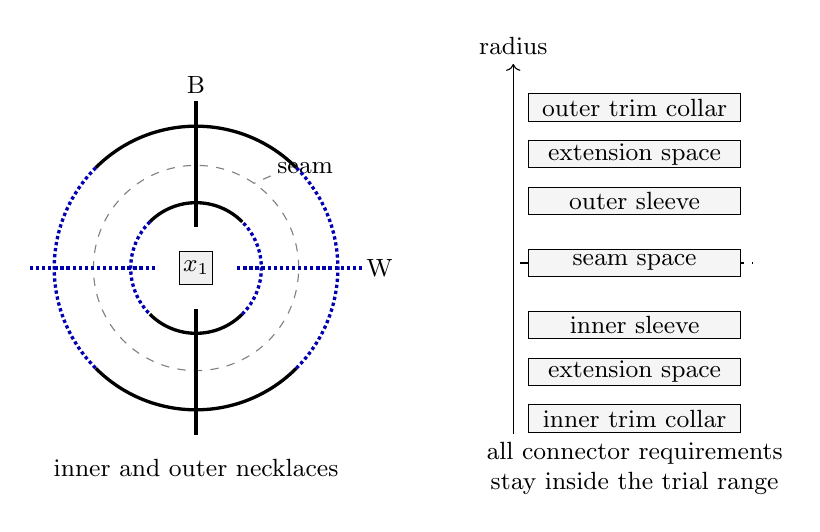
\begin{tikzpicture}[scale=0.79, every node/.style={font=\small}]
  \begin{scope}[xshift=-4.1cm]
    \draw[gray,dashed] (0,0) circle (1.65);
    \node[anchor=west] at (1.15,1.6) {seam};
    \draw[gray,dashed] (1.2,1.48)--(0.93,1.36);
    \foreach \r in {1.05,2.28} {
      \draw[very thick,black] (45:\r) arc (45:135:\r);
      \draw[very thick,blue!70!black,densely dotted] (135:\r) arc (135:225:\r);
      \draw[very thick,black] (225:\r) arc (225:315:\r);
      \draw[very thick,blue!70!black,densely dotted] (315:\r) arc (315:405:\r);
    }
    \draw[very thick,black] (90:0.66)--(90:2.68);
    \draw[very thick,black] (270:0.66)--(270:2.68);
    \draw[very thick,blue!70!black,densely dotted] (0:0.66)--(0:2.68);
    \draw[very thick,blue!70!black,densely dotted] (180:0.66)--(180:2.68);
    \draw[fill=gray!12] (-.27,-.27) rectangle (.27,.27);
    \node at (0,0) {$x_1$};
    \node at (0,2.94) {B};
    \node at (2.95,0) {W};
    \node[align=center] at (0,-3.22) {inner and outer necklaces};
  \end{scope}
  \begin{scope}[xshift=1cm,yshift=-2.42cm]
    \draw[->] (0,-.25)--(0,5.7) node[above] {radius};
    \draw[dashed] (.1,2.5)--(3.85,2.5);
    \foreach \y/\label in {0/inner trim collar,.75/extension space,1.5/inner sleeve,2.5/seam space,3.5/outer sleeve,4.25/extension space,5/outer trim collar} {
      \draw[fill=gray!8] (.25,\y-.22) rectangle (3.65,\y+.22);
      \node at (1.95,\y) {\label};
    }
    \node[align=center] at (1.95,-.8) {all connector requirements\\stay inside the trial range};
  \end{scope}
\end{tikzpicture}
\caption{The sewing construction, drawn schematically with round cycles.
Solid black and dotted blue denote the two colors.  Four ordered arms
carry the connection bit between necklaces across the deterministic seam.
The right-hand diagram gives the radial order of one trial; each displayed
space has fixed multiplicative width, with additional buffers between
supports.  Actual necklaces are site cycles, and the central forced region
is a square.}
\label{fig:sewing}
\end{figure}

For a fixed fair-bit environment, the connection bit at an inner necklace
is a monotone Boolean function $\phi$ of the bit imposed at the first
insertion.  This holds for both a single site and an entire square.  Thus
$\phi$ is constant or the identity.  At several times the same function
acts coordinatewise on the inserted history, because all other bits inside
the necklace are constant across time.

Fix the two environments and all histories at the other insertions.  For
now assume that every inactive-label crossing, if present, is unchanged
by the exchange; we establish this protection below.  Let $f_A(\mathbf h)$ be the
value of the exterior $F$ test when its outer necklace receives history
$\mathbf h$, and let $g_B(b)$ be the value of the exterior $G$ test when its outer
necklace receives bit $b$.  The necklace lemma makes these exterior
functions independent of which inside supplies the transmitted bit.
Write $a_A=\phi_A(1)-\phi_A(0)$ and
$a_B=\phi_B(1)-\phi_B(0)$, so $a_A,a_B\in\{0,1\}$.  Since both weights
are centered, the product of the signed responses before the exchange is
\begin{equation}
 \begin{aligned}
 &\left[\int f_A(\phi_A\circ\mathbf h)\,dw_1(\mathbf h)\right]
 \left[\int g_B(\phi_B(b))\,d\Delta(b)\right]
 \\
 &\qquad=a_Aa_B\left[\int f_A(\mathbf h)\,dw_1(\mathbf h)\right]
             \left[\int g_B(b)\,d\Delta(b)\right].
 \end{aligned}
 \label{eq:signed-bit-factorization}
\end{equation}
Here $\phi_A\circ\mathbf h$ means coordinatewise composition.  If a response
function is constant, centering annihilates its factor; otherwise it is
the identity.  Exchanging the insides exchanges $\phi_A$ and $\phi_B$,
while $f_A,g_B$ and their weights stay with the exterior tests.  The
right-hand side is unchanged.  This is a pointwise equality after the
signed history sums, not an equality between arbitrarily paired raw
histories.  Summing the other histories therefore preserves it.

\subsection{The adaptive exchange and relative error estimates}

Choose finitely many trial annuli with disjoint enlarged supports and a
seam in each.  All lie beyond both first-insertion scales.  Let $A_j$ be
the event that trial $j$ is the first successful trial in a fixed order,
and let $A_0$ be the event that none succeeds.  If $\mathcal T_j$ exchanges the
insides at trial $j$, define
\[
 \mathcal T(\omega^A,\omega^B)=
 \begin{cases}
 \mathcal T_j(\omega^A,\omega^B),&\text{on }A_j,\ j\ge1,\\
 (\omega^A,\omega^B),&\text{on }A_0.
 \end{cases}
\]
Each fixed exchange $\mathcal T_j$ preserves the product law: restrictions of
two independent marked Poisson processes to the inside are independent
and identically distributed, as are their fair bits.  On the lattice the
same observation applies to the bits.  The added nucleus is an annotation
that moves from the site environment to the other environment; no
Poisson intensity or Palm weight is changed.

The success status of trial $j$ is invariant under $\mathcal T_j$.  A trial farther
inside sees its two source environments exchanged wholesale, and a trial
farther outside is unchanged.  The success test is symmetric in its
sources, so every trial's status, and therefore $A_j$, is invariant under
$\mathcal T_j$.  The sets $A_0,A_1,\ldots$ partition the environment space; applying
a measure-preserving involution on each invariant piece proves that $\mathcal T$
is itself a measurable measure-preserving involution on the underlying
unannotated marked environments.  On its successful set it also exchanges
the site--square and square--site annotations.  On $A_0$ the annotations
stay in place, and we estimate that part separately.

We now estimate the error relative to the necessary four-arm probabilities.
First we remove failures of the microscopic screens.  An outer annulus
then protects the inactive replica, while many smaller annuli provide
trials for the active label.  The square radius $h$ will be taken below
all these trials only after their number and positions have been fixed.
Choose a fixed macroscopic probe radius $R$ sufficiently small for the
separations and tested boundaries.  Necessary probes at $x_i$, $i\ge2$,
have disjoint buffered supports from all the constructions at $x_1$;
they always contribute at most $C P_e$.  We therefore estimate only the
two environments at $x_1$.

Fix a large constant $M$.  By the outermost-failure estimate of
Lemma~\ref{lem:localization}, configurations contributing to either signed
product with an occupancy failure at a scale at least $M b_e$ in its site
probe have total probability at most
\begin{equation}
 \varepsilon(M)a_ea_{e,h},\qquad \varepsilon(M)\longrightarrow0.
 \label{eq:site-cutoff-error}
\end{equation}
For the square probe, failures above a constant multiple of $h$ contribute
$o_e(1)a_ea_{e,h}$ at each fixed $h$.  These estimates do not assume arms
on failed shells: group by the outermost failure, retain the necessary
probe beyond it with a disjoint buffer, and apply the power lower bound
and quasi-multiplicativity to sum the lost inner scales.

Outside these errors a necessary event $E$ consists of the occupancy
screens and four alternating active-label graph arms in both environments,
from scales comparable to $M b_e$ and $h$, respectively, to a scale
comparable to $R$.  Use deterministic graph-cycle cuts with room at the
ends.  These arms use the base fair bits: no inserted history reaches any
of their screened probe regions.  Although different crossing coordinates
may witness influence, the first insertion can influence only its active
label, so all these alternatives imply the same event $E$.  In particular
\begin{equation}
 \PP(E)\leq C(M,R)a_ea_{e,h}.
 \label{eq:necessary-probes-upper}
\end{equation}
The definition is made separately with the appropriate site and square
starting scales on the two sides of the comparison.  The event $E$ is
used only for upper bounds; the adaptive exchange is defined by its
symmetric success tests and does not require $E$ to be invariant.

Two ways of keeping these bounds relative will be used repeatedly.
First, let $J$ be a fixed positive-scale intermediate annulus, with
buffers, and let $H_J$ be a geometry event measurable in its enlargement
whose failure probability tends to zero.  Retain the necessary arm probes
strictly below and above that enlargement, in both environments.  These
probes are independent of its geometry.  Quasi-multiplicativity bounds
their product by $C(M,R)a_ea_{e,h}$ divided by the two fixed-ratio arm
costs omitted at $J$.  Those costs have positive mesh-uniform lower
bounds.  It follows that
\begin{equation}
 \PP(E\cap H_J^c)=o_e(1)a_ea_{e,h}.
 \label{eq:relative-typical-geometry}
\end{equation}
This also applies to geometry requirements in a sewn combination: a fixed
inside--outside combination has the ordinary Poisson law, and its local
geometry is still measurable in the two enlarged source annuli.  A finite
list of all such requirements is typical.  No typicality assertion is
being made at the microscopic scale $b_e$.

Second, choose $l_*>0$ much smaller than $R$ and put all trial annuli
strictly below $l_*$, with buffers.  When two replicas are used, impose the
following \emph{protection event} $H$: screening holds on an annulus from
constant multiples of $l_*$ to constant multiples of $R$, and in neither
source environment does the inactive label have four alternating arms
through that annulus.  It uses only sites above all the seams, hence is
invariant under every exchange.  If a tested crossing of the inactive
label changed after an exchange, the two configurations would agree on
this annulus and differ only on its inside.  The pivotal arm implication
would then give the forbidden four arms there.  The argument works for
every setting of the other histories, which are all outside the probe,
and includes changes of cells caused by the exchanged geometry.

For completeness, conditioning on the common geometry within this probe,
the two labels are independent.  If $p_e(\eta)$ is its quenched active
four-arm probability, the probability of four arms for both labels is
$\EE[p_e(\eta)^2]$, bounded by
$C A_e(l_*,R)^2$ by the second-moment arm estimate.  Retain the active
probe below it and the necessary probe in the other environment with
disjoint buffers.  Quasi-multiplicativity then gives
\begin{equation}
 \PP(E\cap H^c)
 \leq \bigl[C(M,R)A_e(l_*,R)+o_e(1)\bigr]a_ea_{e,h}.
 \label{eq:inactive-protection}
\end{equation}
Sum over which of the two source environments fails protection.  Fixed
radius changes are absorbed into the constant; mesh failures are covered
by \eqref{eq:relative-typical-geometry}.  The power upper bound makes the
bracket as small as desired by choosing $l_*/R$ small and then the mesh
small.  This extra arm factor is the reason common Poisson geometry for
the two replicas is compatible with the exchange argument.  With one
replica set $H$ equal to the entire probability space.

\subsection{Many annular trials}

It remains to show that $E$ almost always supplies a successful seam on
the relative scale $a_ea_{e,h}$.  Each trial has the radial layout in
Figure~\ref{fig:sewing}: an inner trim collar, an extension space, an inner
sleeve, a seam space, an outer sleeve, another extension space, and an
outer trim collar.  Every part has a fixed sufficiently large ratio.
Trim curves run through the middle of their collars; the deterministic
seam runs through the middle of its space.  The sleeve ratio is that of
Lemma~\ref{lem:necklace-sleeve}.  Include buffers between supports, and
choose all endpoint boxes and corridor routes from finite lists scaled
with the trial.  For any fixed number $n$, one can place $n$ such similar,
buffered trials below $l_*$ at fixed positive scales.  Subsequently take
$h$ below the innermost trial.

For trial $J$, let $T_J$ be the typical geometry event giving all its
screens, the quenched lower bounds for both sleeve constructions in both
environments, and all the
rectangle-crossing lower bounds for the corridor lists in every possible
sewn combination.  Screens in particular make each sleeve independent
of the source used on the far side of the seam.  Each sewn geometry has
the ordinary law, so a finite intersection supplies $T_J$.
Call $J$ \emph{disqualified}, an event denoted $B_J$, if $T_J$ fails or a
bad trim occurs at either of its two trim curves in either environment.
The bad trim test is the local close-approach event of
Lemma~\ref{lem:trim-arms}, including extra visits near the reserved
endpoint boxes.  Its paths are proper simple arms through a wider collar;
thus the two visits giving the test really yield four arms in a buffered
neighborhood, regardless of their color order.

For any $\rho>0$, the trim tolerance and the local geometry requirements
can be chosen so that, for every trial,
\begin{equation}
 \limsup_{e\downarrow0}
 \frac{\PP(E\cap B_J)}{a_ea_{e,h}}\leq\rho.
 \label{eq:trial-disqualification}
\end{equation}
Here and below $h$ is fixed below the trials.  For geometry failures this
is \eqref{eq:relative-typical-geometry}.  For a bad trim retain the
necessary parts of that environment's probe on both sides of its collar,
and the other environment's probe.  Their supports, including Poisson
buffers, avoid the bad test.  The absolute close-approach probability
multiplies their arm costs; deleting the fixed-ratio collar costs only a
fixed factor by quasi-multiplicativity.  Choose its tolerance to absorb
that factor.  This reasoning is uniform over scaled copies of the trial:
$\rho$ and the construction constants do not depend on $n$ or on a trial's
radius.  The mesh threshold may depend on the fixed finite collection.

Write $U_J$ for the symmetric successful seam event in trial $J$, and
$N=\bigcap_J U_J^c$ for failure of every trial.  The trials cannot be
treated as independent after restricting to the necessary long-arm event
$E$.  Instead, we compare failure of every trial with success of exactly
one specified trial.  The latter events are disjoint as that trial varies,
which will give the gain from the number of trials.

\begin{lemma}[One-trial comparison]
\label{lem:one-trial}
For the preceding fixed layouts and tolerances, there is $C_*<\infty$,
independent of the number of trials, their scales, and sufficiently small
mesh, such that
\begin{equation}
 \PP(E\cap N\cap B_J^c)
 \leq C_*\,
 \PP\left(E\cap U_J\cap\bigcap_{I\ne J}U_I^c\right)
 \label{eq:one-trial-comparison}
\end{equation}
for every trial $J$.
\end{lemma}

\begin{proof}
Condition first on all Poisson geometries, keeping only realizations in
$T_J$ and in the geometry part of $E$.  In each source environment retain
four arms from the inner beginning of its probe to the inner trim curve,
and four arms from its outer end down to the outer trim curve.  Stop at
first contact from the retained side, with the graph margins prescribed
above.  Since the trim is not bad, their endpoint boxes can be chosen from
a fixed finite list with matching cyclic order and the reserved avoidance
conditions.  For each choice let $\mathcal R$ be the event that such retained paths
exist, together with failure of all trials other than $J$.  Delete the
color part of disqualification, failure of trial $J$, and all arm
requirements between its two trims.  The events $\mathcal R$ for the finitely many
box and order choices cover the left-hand event of
\eqref{eq:one-trial-comparison}.  Their definition concerns existence of
retained paths; we do not reveal or condition on a selected path.

In the four sleeves, two in each source environment, impose the events
of Lemma~\ref{lem:necklace-sleeve}, with cardinal endpoint patches of
matching alternating colors.  Sleeve coordinates are disjoint from the
retained path coordinates and from the other trial supports.  Thus these
four events have joint conditional probability at least $c_0^4$, and
intersecting them with $\mathcal R$ costs at most that fixed factor.

We describe precisely the additional connector supports.  In each
extension space use disjoint polygonal tracks from the retained endpoint
boxes to the corresponding sleeve patches, first leaving the trim in its
normal direction and then respecting annular cyclic order.  At each end
start a track inside the box surrounded by the guarded lasso.  In the
seam space use four fixed separated tracks, of the same respective
colors for every inside--outside combination, and require rectangle-chain
connections in each of its four sewn geometries.  Every rectangle and
lasso used by a connector lies in these tracks or in a reserved endpoint
enlargement.  Include their cell stars in the supports.

Let $V_{\rm B}$ and $V_{\rm W}$ be, respectively, the original source-bit
coordinates used by black and white connector requirements, taking the
union over the four sewn combinations.  The positive widths between
opposite-color tracks and the mesh screens ensure
$V_{\rm B}\cap V_{\rm W}=\varnothing$; a source site cannot belong to two
opposite track supports, even if it is used in several sewn geometries.
On $V=V_{\rm B}\cup V_{\rm W}$ put the product order that favors black
on $V_{\rm B}$ and white on $V_{\rm W}$.  Every connector event is
increasing in this order.  Its conditional probability, with geometries
fixed, has a uniform positive lower bound from the crossing conditions
in $T_J$.  Harris' inequality therefore bounds the probability of all
connector events by a positive constant from below, since their number
is fixed.  These events depend only on the coordinates in $V$.

The retained-and-sleeve event has the same monotonicities on $V$.
For retained paths the only overlaps are their reserved, color-specific
endpoint enlargements.  For sleeves the only overlaps are their guarded
end patches; the five-arm exclusion giving the necklace lies strictly
in the core and uses no coordinate of $V$.  Requirements that paths avoid
other boxes are restrictions on allowed path locations, so favoring their
own colors preserves the existence of the required paths.  Failures of
other trials use no coordinate of $V$, or of these sleeves, because the
enlarged trial supports are disjoint.  They need not be monotone.

Now condition on all color coordinates outside $V$, apply Harris in $V$
to the retained-and-sleeve event and the intersection of the connector
events, and integrate back.  This costs another fixed positive factor.
All joining requirements are realized simultaneously, including those
in geometries that combine different sources.  Lassos ensure actual
connections to retained paths, while the reserved tracks ensure
disjointness, including between arms of the same color.  In the two
original environments the resulting arms complete $E$.  In all four
combinations they give $U_J$, with the common necklaces supplied by the
sleeves.  Other trials still fail.  Hence the probability for each retained
choice is at most a constant times the right-hand probability in
\eqref{eq:one-trial-comparison}.  Summing over the bounded finite choices
and then integrating the geometries proves the claim.
\end{proof}

Summing \eqref{eq:one-trial-comparison} over $n$ trials, its right-hand
events are pairwise disjoint.  On the left,
\[
 n\PP(E\cap N)
 \leq \sum_J\PP(E\cap N\cap B_J^c)+\sum_J\PP(E\cap B_J).
\]
Together with \eqref{eq:necessary-probes-upper} and
\eqref{eq:trial-disqualification}, this gives
\begin{equation}
 \limsup_{e\downarrow0}
 \frac{\PP(E\cap N)}{a_ea_{e,h}}
 \leq \rho+\frac{C_* C(M,R)}{n}.
 \label{eq:many-trials}
\end{equation}
The averaging over disqualifications, rather than a union bound over all
of them, is what leaves $\rho$ instead of $n\rho$.

\begin{proof}[Proof of Proposition~\ref{prop:replacement}]
Choose a desired relative error $z>0$.  First fix $M$ so that the cutoff
error in \eqref{eq:site-cutoff-error} is sufficiently small.  Next choose
$l_*/R$ so that \eqref{eq:inactive-protection} is sufficiently small.
Fix the sleeve and extension ratios, and the trim tolerances so that the
disqualification term $\rho$ is sufficiently small.  These choices fix
$C_*$.  Choose $n$ so large that $C_*C(M,R)/n$ is sufficiently small,
and place that many buffered trials below the protection annulus.
Only now take $h$ sufficiently small to lie below every trial; for each
such fixed $h$, let $e\downarrow0$.  All local constructions are therefore
at positive scales when their geometry conditions are imposed.

On configurations with a successful protected seam, the adaptive
measure-preserving involution and the signed identity following
Lemma~\ref{lem:necklace-bit} identify the two product integrals.
The remaining portions are bounded in total variation.  A nonzero
signed contribution has the necessary probes at every insertion point;
the independent probes at the other points contribute $C P_e$.  At the
first point the discarded portions are bounded by
\eqref{eq:site-cutoff-error}, \eqref{eq:inactive-protection}, and
\eqref{eq:many-trials}, together with the vanishing fixed-scale geometry
errors.  The weights contribute only their fixed total-variation bounds.
Thus the limsup of the ratio in
\eqref{eq:signed-relative-replacement} is at most $Cz$; since $z$ is
arbitrary, it is zero.

All constants are uniform on the fixed compact separated location range.
Local layouts are translated copies of the same finite lists.  In the
Poisson model Mecke points at other insertions lie outside their buffered
supports, and the screens make those annotations irrelevant there.  In
the triangular model translations are by lattice sites.  This proves
the stated uniformity and completes the comparison.
\end{proof}

\section{Identification and the quenched limit}
\label{sec:identification}

The expansion and local comparison now identify the law.  At the
auxiliary scale $q_e$, the first derivative of the $Q_0$ crossing
probability is exactly one at criticality.  Its square-insertion
approximation has a common critical limit, so this identity determines the unknown
site-to-square comparison factor.  We then identify every finite
crossing test, convert from the rectangle to the unit-square
normalization, and pass to the conditional law on $\mathcal K$.
All quantities indexed by $e$ in this section are formed separately
in each model, with the notation of
Sections~\ref{sec:expansion} and~\ref{sec:sewing}.

\subsection{Calibration by one crossing derivative}

Recall that $q_e=(\EE N_e(Q_0))^{-1}$ for the centered auxiliary
rectangle $Q_0$. For its translate centered at a proposed insertion
point, let $S_e$ be the critical single-site kernel and $D_e(h)$ the
critical square-insertion kernel, both with weight
$\delta_1-\delta_0$. These are the nonnegative quantities introduced
in Section~\ref{sec:sewing}. Put
\begin{equation}
 c_e=m_e q_e S_e.
 \label{eq:amplitude-ratio}
\end{equation}
The arm upper bound on $S_e$, together with
$q_e\asymp(m_e a_e)^{-1}$, shows that $c_e$ is bounded.

\begin{lemma}[Common calibration]
\label{lem:common-calibration}
There is a constant $c\in(0,\infty)$ such that $c_e\to c$ in both
models. Moreover, for each fixed degree, assignment of one replica
label to each insertion, and finite signed crossing test, its normalized
all-site kernel integral has a limit common to the two models.
\end{lemma}

\begin{proof}
Fix a compact range of insertion locations separated from one another
and from all polygon boundaries. Write $K_{e,s}(x_1,\ldots,x_k)$ for
the all-site kernel and $K_{e,h}(x_1,\ldots,x_k)$ for the kernel with
all insertions replaced by squares of radius $h$.
Proposition~\ref{prop:replacement}, applied successively at the $k$
locations, gives
\begin{equation}
 (m_e q_e)^k K_{e,s}(\boldsymbol x)
 =c_e^k\frac{K_{e,h}(\boldsymbol x)}{D_e(h)^k}
       +o_h(1),
 \label{eq:all-disk-replacement}
\end{equation}
uniformly on this range, in the ordered sense
$\lim_{h\downarrow0}\limsup_{e\downarrow0}|o_h(1)|=0$.
Here and below a kernel includes its specified signed weights.
To check the factors in this iteration, divide the single replacement
estimate by $D_e(h)\ge c_0 a_{e,h}$. Each already replaced location
contributes at most
$S_e/D_e(h)\le C a_e/a_{e,h}$, while its square kernel costs
$C a_{e,h}$. Thus every accumulated error is $o_h(a_e^k)$ before
normalization. The bound $m_e q_e a_e\le C$ proves
\eqref{eq:all-disk-replacement}, including when $c_e$ is small.

For fixed sufficiently small $h$, Proposition~\ref{prop:critical-tests}
gives common critical limits for $K_{e,h}$ and $D_e(h)$.
The limiting denominator is positive: the square lower bound and the
four-arm lower power bound give $D_e(h)\ge c_h>0$ at this fixed $h$.
These limits hold also for convergent insertion locations and are
continuous on the separated range. Consequently the convergence is
uniform there. Indeed, a failure of uniform convergence would give
a sequence of locations with a convergent subsequence, contradicting
the assertion for convergent locations. Since $\sigma_e$ converges
to Lebesgue measure, integrals against a fixed continuous cutoff
therefore converge too. This applies to the triangular counting
measure as well as to the Poisson location integral.

Apply this observation first with $k=1$, $F=\mathbf1_{C_{Q_0}}$, and
weight $\delta_1-\delta_0$. Its full normalized first coefficient is
\begin{equation}
 m_e q_e\int K_{e,s}(x)\,d\sigma_e(x)
       =q_e\EE N_e(Q_0)=1.
 \label{eq:coefficient-one}
\end{equation}
One may first use the localized box from
Section~\ref{sec:expansion}; its omission contributes $o(1)$ also to
this coefficient. By Lemma~\ref{lem:location-ui}, for every $z>0$
there is a continuous cutoff $0\le\chi\le1$, supported on a compact
range away from the polygon boundary and the box boundary, such that
the integral in \eqref{eq:coefficient-one} changes by at most $z+o(1)$
when multiplied by $\chi$. Nonnegativity is used here.

Let $J_\chi(h)$ be the common limit of
\[
 \int\chi(x)\frac{K_{e,h}(x)}{D_e(h)}\,d\sigma_e(x).
\]
The separate insertion upper bound and the square lower bound imply
$0\le J_\chi(h)\le C_\chi$, uniformly for sufficiently small $h$.
For any subsequential limit $c_*$ of $c_e$,
\begin{equation}
 |1-c_*J_\chi(h)|\le z+o_h(1).
 \label{eq:calibration-cutoff}
\end{equation}
Choose $z<1/4$ and then $h$ small. This proves that every such $c_*$
is bounded below by a positive constant. If $c_+$ and $c_-$ are two
subsequential limits, possibly from different models, the same cutoff
and the same $J_\chi(h)$ work for both. Since all $c_e$ have a common
upper bound $C$, \eqref{eq:calibration-cutoff} also gives
$J_\chi(h)\ge(1-z-o_h(1))/C$. Subtracting the two instances yields
\[
 |c_+-c_-|\le
 \frac{2C(z+o_h(1))}{1-z-o_h(1)}.
\]
First let $h\downarrow0$ and then $z\downarrow0$.
All subsequential limits agree, proving $c_e\to c>0$.

For a general fixed coefficient, restrict its location integral to
a compact separated range, losing at most an arbitrarily small
amount by Lemma~\ref{lem:location-ui}. Equation~\eqref{eq:all-disk-replacement}
and the common critical square limits compare any two subsequential
limits of the restricted coefficient. Their difference tends to zero
as $h\downarrow0$. Removing the cutoff proves uniqueness of the full
coefficient limit across both models. Boundedness follows from
Proposition~\ref{prop:expansion-bound}, so these limits exist.
The factor $1/k!$ in the expansion and the finite sum over replica
assignments do not affect this argument.
\end{proof}

This calibration uses a common macroscopic test, rather than a
comparison of the microscopic scales at equal numerical mesh.
We next convert it to the unit-square normalization of the theorem.

\begin{lemma}[The prescribed normalization]
\label{lem:square-normalization}
There is a common constant $B\in(0,\infty)$ such that, in each model,
\begin{equation}
 q_e\EE N_e(Q_*)\longrightarrow B,
 \qquad r_e=\frac{q_e}{B+o(1)}.
 \label{eq:square-normalization}
\end{equation}
In particular, both prescribed scales tend to zero.
\end{lemma}

\begin{proof}
The first expression is the normalized first coefficient of
$\mathbf1_{C_{Q_*}}$ with weight $\delta_1-\delta_0$.
Lemma~\ref{lem:common-calibration} gives a common finite limit $B$.
For positivity restrict insertion locations to a small open patch
near the center of $Q_*$. The square lower bound of
Lemma~\ref{lem:disk-lower} gives
$K_{e,h}(x)\ge c_1 a_{e,h}$ uniformly on a smaller patch, whereas
$D_e(h)\le C_1a_{e,h}$. Choose a nonzero nonnegative cutoff in that
patch. Equation~\eqref{eq:all-disk-replacement} with $k=1$ and $c_e\to c>0$
shows that this part of the limiting first coefficient is strictly
positive. All omitted parts are nonnegative. Hence $B>0$.
Taking reciprocals gives \eqref{eq:square-normalization};
$q_e\to0$ by Lemma~\ref{lem:pivotal-scale}.
\end{proof}

\subsection{Finite tests and threshold laws}

\begin{proposition}[Common finite-time crossing limits]
\label{prop:nearcritical-tests}
Choose finitely many quads in $\mathcal Q_{\mathrm{rat}}$ and finitely
many real parameters. Their jointly coupled crossing indicators,
with the prescribed scales $r_e$, have a limiting law common to the
two models. The assertion holds for one color replica and for two
independent color replicas conditional on the same geometry.
Every such limiting probability is continuous in the real parameter
vector, and the convergence remains valid for convergent parameter
vectors.
\end{proposition}

\begin{proof}
First use the auxiliary scale $q_e$. Expand the expectation of any
bounded function of the specified indicators as in
Section~\ref{sec:expansion}. The degree-zero term has its common critical limit by
Proposition~\ref{prop:critical-tests}, and every positive-degree
coefficient has a common limit by Lemma~\ref{lem:common-calibration}. The terms with repeated
replica labels at one spatial site tend to zero. The majorant in
Proposition~\ref{prop:expansion-bound} is summable uniformly on every
bounded parameter range, so the whole expectation has a common limit.

At fixed degree the history weights are continuous on their finite
labeled history space, including when times coincide or change order.
The kernel integrals are multilinear in these weights. They therefore
have continuous limiting coefficients, and local uniform summability
makes their sum continuous. The same argument applies to convergent
parameter vectors.

At the prescribed scale, the parameter $\lambda$ corresponds to
$t=\lambda/(B+o(1))$ at the auxiliary scale, by
Lemma~\ref{lem:square-normalization}. The conclusion for convergent
vectors proves the assertion in the required normalization.
\end{proof}

\begin{proof}[Proof of Theorem~\ref{thm:main}]
Finiteness and positivity of the expectations follow from
Lemma~\ref{lem:pivotal-scale}; their inverse scales vanish by
Lemma~\ref{lem:square-normalization}.

At fixed mesh, only finitely many cells meet any particular quad
almost surely. Its crossing indicator is monotone in the parameter,
and the closed mark rule gives, at every finite deterministic $t$,
\begin{equation}
 \{\tau_e(Q)\le t\}=\{C_Q\text{ occurs at }p_e(t)\}
 \quad\text{almost surely}.
 \label{eq:cdf-crossing}
\end{equation}
Thus Proposition~\ref{prop:nearcritical-tests} supplies common limits
of the joint distribution functions of every finite set of thresholds.
These limits are continuous at finite parameter vectors.

For completeness, compactification introduces no ambiguity.
Take any weakly convergent subsequence of threshold laws on $\mathcal K$,
which exists by compactness. At finite continuity points of a limiting
coordinate marginal, \eqref{eq:cdf-crossing} identifies its distribution
function with the continuous limiting crossing function. Squeezing
between such continuity points excludes a finite atom and gives the
same identity at every finite point. Apply this to each coordinate
of a finite projection. Its joint distribution function then agrees
with the one supplied by Proposition~\ref{prop:nearcritical-tests}.
Finite-endpoint rectangles determine measures on
$\overline\RR^k$ as well: their increasing or decreasing limits recover
events involving either endpoint at infinity. All finite projections
are therefore uniquely determined. Since the index set is countable,
they determine the law on $\mathcal K$.

In particular, the triangular laws have a full weak limit, which we
denote by $\nu_\triangle$. The annealed one-replica Voronoi laws have
the same limit. Apply the preceding argument also to two replicas.
For the triangular model their joint law is a product at every mesh,
so its limit is $\nu_\triangle\otimes\nu_\triangle$. Proposition~\ref{prop:nearcritical-tests}
shows that two color replicas on a common Poisson geometry have
this same limit.

Let $f$ be a real continuous function on $\mathcal K$, and put
\[
 Z_{e,f}=\EE[f(\tau_e^V)\mid\eta_e],
 \qquad m_f=\int f\,d\nu_\triangle.
\]
Conditional independence of the two color replicas gives
\[
 \EE Z_{e,f}\longrightarrow m_f,
 \qquad
 \EE Z_{e,f}^{2}
 =\EE[f(\tau_e^{V,1})f(\tau_e^{V,2})]
 \longrightarrow m_f^2.
\]
Hence $Z_{e,f}\to m_f$ in $L^2$ over geometry.

The family
$\mathcal F=\{f:\|f\|_\infty\le1,\ \Lip_{d_{\mathcal K}}(f)\le1\}$
is uniformly bounded and equicontinuous on compact $\mathcal K$.
For any $\zeta>0$ it has a finite uniform $\zeta$-net
$f_1,\ldots,f_m$. For every sampled geometry,
\[
 d_{\mathrm{BL}}\bigl(\Law(\tau_e^V\mid\eta_e),\nu_\triangle\bigr)
 \le 2\zeta+\max_{1\le i\le m}|Z_{e,f_i}-m_{f_i}|.
\]
The maximum tends to zero in probability. Letting $\zeta\downarrow0$
proves \eqref{eq:main-quenched}. All arguments apply along arbitrary
vanishing-mesh sequences, completing the proof.
\end{proof}

\begin{thebibliography}{99}

\bibitem{ahlbergbaldasso18}
D. Ahlberg and R. Baldasso,
\emph{Noise sensitivity and Voronoi percolation},
Electron. J. Probab. \textbf{23} (2018), paper no.~108, 21~pp.
\href{https://doi.org/10.1214/18-EJP233}{doi:10.1214/18-EJP233}.

\bibitem{ahlberg-riva-griffiths21}
D. Ahlberg, D. de la Riva, and S. Griffiths,
\emph{On the rate of convergence in quenched Voronoi percolation},
Electron. J. Probab. \textbf{26} (2021), paper no.~143, 26~pp.
\href{https://doi.org/10.1214/21-EJP712}{doi:10.1214/21-EJP712}.

\bibitem{agmt16}
D. Ahlberg, S. Griffiths, R. Morris, and V. Tassion,
\emph{Quenched Voronoi percolation},
Adv. Math. \textbf{286} (2016), 889--911.
\href{https://doi.org/10.1016/j.aim.2015.09.005}{doi:10.1016/j.aim.2015.09.005}.

\bibitem{ahlbergsteif17}
D. Ahlberg and J. E. Steif, with an appendix by G. Pete,
\emph{Scaling limits for the threshold window: When does a monotone
Boolean function flip its outcome?},
Ann. Inst. H. Poincar\'e Probab. Statist. \textbf{53} (2017), no.~4,
2135--2161.
\href{https://doi.org/10.1214/16-AIHP786}{doi:10.1214/16-AIHP786}.

\bibitem{aizenmanburchard99}
M. Aizenman and A. Burchard,
\emph{H\"older regularity and dimension bounds for random curves},
Duke Math. J. \textbf{99} (1999), no.~3, 419--453.
\href{https://doi.org/10.1215/S0012-7094-99-09914-3}{doi:10.1215/S0012-7094-99-09914-3}.

\bibitem{bks99}
I. Benjamini, G. Kalai, and O. Schramm,
\emph{Noise sensitivity of boolean functions and applications to
percolation},
Publ. Math. Inst. Hautes \'Etudes Sci. \textbf{90} (1999), 5--43.
\href{https://doi.org/10.1007/BF02698830}{doi:10.1007/BF02698830}.

\bibitem{bollobasriordan06}
B. Bollob\'as and O. Riordan,
\emph{The critical probability for random Voronoi percolation in the
plane is $1/2$},
Probab. Theory Related Fields \textbf{136} (2006), no.~3, 417--468.
\href{https://doi.org/10.1007/s00440-005-0490-z}{doi:10.1007/s00440-005-0490-z}.

\bibitem{cnloops}
F. Camia and C. M. Newman,
\emph{Two-dimensional critical percolation: the full scaling limit},
Comm. Math. Phys. \textbf{268} (2006), no.~1, 1--38.
\href{https://doi.org/10.1007/s00220-006-0086-1}{doi:10.1007/s00220-006-0086-1}.

\bibitem{cnexploration}
F. Camia and C. M. Newman,
\emph{Critical percolation exploration path and SLE$_6$: a proof of
convergence},
Probab. Theory Related Fields \textbf{139} (2007), nos.~3--4, 473--519.
\href{https://doi.org/10.1007/s00440-006-0049-7}{doi:10.1007/s00440-006-0049-7}.

\bibitem{cardy92}
J. L. Cardy,
\emph{Critical percolation in finite geometries},
J. Phys. A: Math. Gen. \textbf{25} (1992), no.~4, L201--L206.
\href{https://doi.org/10.1088/0305-4470/25/4/009}{doi:10.1088/0305-4470/25/4/009}.

\bibitem{gps-fourier}
C. Garban, G. Pete, and O. Schramm,
\emph{The Fourier spectrum of critical percolation},
Acta Math. \textbf{205} (2010), no.~1, 19--104.
\href{https://doi.org/10.1007/s11511-010-0051-x}{doi:10.1007/s11511-010-0051-x}.

\bibitem{garbanpete-schramm-pivotal}
C. Garban, G. Pete, and O. Schramm,
\emph{Pivotal, cluster, and interface measures for critical planar
percolation},
J. Amer. Math. Soc. \textbf{26} (2013), no.~4, 939--1024.
\href{https://doi.org/10.1090/S0894-0347-2013-00772-9}{doi:10.1090/S0894-0347-2013-00772-9}.

\bibitem{garbanpete-schramm-nearcritical}
C. Garban, G. Pete, and O. Schramm,
\emph{The scaling limits of near-critical and dynamical percolation},
J. Eur. Math. Soc. \textbf{20} (2018), no.~5, 1195--1268.
\href{https://doi.org/10.4171/JEMS/786}{doi:10.4171/JEMS/786}.

\bibitem{harris60}
T. E. Harris,
\emph{A lower bound for the critical probability in a certain
percolation process},
Proc. Cambridge Philos. Soc. \textbf{56} (1960), no.~1, 13--20.
\href{https://doi.org/10.1017/S0305004100034241}{doi:10.1017/S0305004100034241}.

\bibitem{kesten87}
H. Kesten,
\emph{Scaling relations for 2D-percolation},
Comm. Math. Phys. \textbf{109} (1987), no.~1, 109--156.
\href{https://doi.org/10.1007/BF01205674}{doi:10.1007/BF01205674}.

\bibitem{nolin08}
P. Nolin,
\emph{Near-critical percolation in two dimensions},
Electron. J. Probab. \textbf{13} (2008), paper no.~55, 1562--1623.
\href{https://doi.org/10.1214/EJP.v13-565}{doi:10.1214/EJP.v13-565}.

\bibitem{supplied-cardy}
OpenAI,
\emph{Cardy's formula for critical Poisson--Voronoi percolation},
OpenAI Math Release preprint
\href{https://github.com/openai/math/blob/main/preprints/Cardys-formula-for-critical-Poisson-Voronoi-percolation-September-23-2026/paper.pdf}{OAI:Cardys-formula-for-critical-Poisson-Voronoi-percolation-September-23-2026},
2026.

\bibitem{reimer00}
D. Reimer,
\emph{Proof of the Van den Berg--Kesten conjecture},
Combin. Probab. Comput. \textbf{9} (2000), no.~1, 27--32.
\href{https://doi.org/10.1017/S0963548399004113}{doi:10.1017/S0963548399004113}.

\bibitem{russo78}
L. Russo,
\emph{A note on percolation},
Z. Wahrscheinlichkeitstheorie verw. Gebiete \textbf{43} (1978), no.~1,
39--48.
\href{https://doi.org/10.1007/BF00535274}{doi:10.1007/BF00535274}.

\bibitem{schramm00}
O. Schramm,
\emph{Scaling limits of loop-erased random walks and uniform spanning
trees},
Israel J. Math. \textbf{118} (2000), 221--288.
\href{https://doi.org/10.1007/BF02803524}{doi:10.1007/BF02803524}.

\bibitem{schrammsmirnov11}
O. Schramm and S. Smirnov, with an appendix by C. Garban,
\emph{On the scaling limits of planar percolation},
Ann. Probab. \textbf{39} (2011), no.~5, 1768--1814.
\href{https://doi.org/10.1214/11-AOP659}{doi:10.1214/11-AOP659}.

\bibitem{seymourwelsh78}
P. D. Seymour and D. J. A. Welsh,
\emph{Percolation probabilities on the square lattice},
Ann. Discrete Math. \textbf{3} (1978), 227--245.
\href{https://doi.org/10.1016/S0167-5060(08)70509-0}{doi:10.1016/S0167-5060(08)70509-0}.

\bibitem{smirnov01}
S. Smirnov,
\emph{Critical percolation in the plane: conformal invariance, Cardy's
formula, scaling limits},
C. R. Acad. Sci. Paris S\'er. I Math. \textbf{333} (2001), no.~3,
239--244.
\href{https://doi.org/10.1016/S0764-4442(01)01991-7}{doi:10.1016/S0764-4442(01)01991-7}.

\bibitem{smirnovwerner01}
S. Smirnov and W. Werner,
\emph{Critical exponents for two-dimensional percolation},
Math. Res. Lett. \textbf{8} (2001), 729--744.
\href{https://doi.org/10.4310/MRL.2001.v8.n6.a4}{doi:10.4310/MRL.2001.v8.n6.a4}.

\bibitem{tassion16}
V. Tassion,
\emph{Crossing probabilities for Voronoi percolation},
Ann. Probab. \textbf{44} (2016), no.~5, 3385--3398.
\href{https://doi.org/10.1214/15-AOP1052}{doi:10.1214/15-AOP1052}.

\bibitem{vandenbergkesten85}
J. van den Berg and H. Kesten,
\emph{Inequalities with applications to percolation and reliability},
J. Appl. Probab. \textbf{22} (1985), no.~3, 556--569.
\href{https://doi.org/10.2307/3213860}{doi:10.2307/3213860}.

\bibitem{vanneuville-scaling}
H. Vanneuville,
\emph{Annealed scaling relations for Voronoi percolation},
Electron. J. Probab. \textbf{24} (2019), paper no.~39, 71~pp.
\href{https://doi.org/10.1214/19-EJP293}{doi:10.1214/19-EJP293}.

\bibitem{vanneuville-spectral}
H. Vanneuville,
\emph{The annealed spectral sample of Voronoi percolation},
Ann. Probab. \textbf{49} (2021), no.~3, 1554--1606.
\href{https://doi.org/10.1214/20-AOP1494}{doi:10.1214/20-AOP1494}.

\bibitem{vanneuville-quantitative}
H. Vanneuville,
\emph{Quantitative quenched Voronoi percolation and applications},
Ann. Inst. Fourier (Grenoble) \textbf{75} (2025), no.~4, 1649--1683.
\href{https://doi.org/10.5802/aif.3710}{doi:10.5802/aif.3710}.

\end{thebibliography}

\end{document}
